\documentclass[12pt,a4paper]{report}
%use larger type; default would be 10pt
%\usepackage[lining,semibold,type1]{libertine}
\counterwithout{figure}{chapter}
\counterwithout{equation}{chapter}
\usepackage{amsmath,amssymb,amsthm}
%\usepackage{libertine}
%\usepackage{libertinust1math}
\usepackage[T1]{fontenc}
\usepackage[utf8]{inputenc} % set input encoding (not needed with XeLaTeX)
\usepackage{indentfirst}
\usepackage[dvipsnames]{xcolor}
\definecolor{gray}{rgb}{0.85,0.85,0.85}
\definecolor{codegreen}{rgb}{0,0.6,0}
\definecolor{codegray}{rgb}{0.5,0.5,0.5}
\definecolor{codepurple}{rgb}{0.58,0,0.82}
\definecolor{backcolour}{rgb}{0.95,0.95,0.92}
\usepackage{listings}
\lstset{language=Octave,
	backgroundcolor=\color{white},   % choose the background color; you must add \usepackage{color} or \usepackage{xcolor}
	basicstyle=\footnotesize,%\ttfamily,        % the size of the fonts that are used for the code
	breakatwhitespace=false,         % sets if automatic breaks should only happen at whitespace
	breaklines=true,                 % sets automatic line breaking
	captionpos=b,                    % sets the caption-position to bottom
	commentstyle=\color{codegreen},    % comment style
	%escapeinside={\%*}{*)},          % if you want to add LaTeX within your code
	extendedchars=true,            % lets you use non-ASCII characters; for 8-bits encodings only, does not work with UTF-8
	frame=single,                    % adds a frame around the code
	% frameround=fttt,
	keepspaces=true,                 % keeps spaces in text, useful for keeping indentation of code (possibly needs columns=flexible)
	classoffset=0,
	keywordstyle=\color{black},%\color{RoyalBlue},       % keyword style
	deletekeywords={function,endfunction, if,endif},
	classoffset=1,
	morekeywords={function,endfunction, if,endif},
	keywordstyle=\bf\color{Red},       % keyword style
	classoffset=2,
	morekeywords={persistent},            % if you want to add more keywords to the set
	keywordstyle=\bf\color{ForestGreen},       % keyword style
	classoffset=0,
	literate=
	{/}{{{\color{Mahogany}/}}}1
	{*}{{{\color{Mahogany}*}}}1
	{.*}{{{\color{Mahogany}.*}}}2
	{+}{{{\color{Mahogany}+{}}}}1
	{=}{{{\bf\color{Mahogany}=}}}1
	{-}{{{\color{Mahogany}-}}}1
	{[}{{{\bf\color{RedOrange}[}}}1
	{]}{{{\bf\color{RedOrange}]}}}1
	{ç}{{\c{c}}}1 % Cedilha
	{á}{{\'{a}}}1 % Acentos agudos
	{é}{{\'{e}}}1
	{í}{{\'{i}}}1
	{ó}{{\'{o}}}1
	{ú}{{\'{u}}}1
	{â}{{\^{a}}}1 % Acentos circunflexos
	{ê}{{\^{e}}}1
	{î}{{\^{i}}}1
	{ô}{{\^{o}}}1
	{û}{{\^{u}}}1
	{à}{{\`{a}}}1 % Acentos graves
	{è}{{\`{e}}}1
	{ì}{{\`{i}}}1
	{ò}{{\`{o}}}1
	{ù}{{\`{u}}}1
	{ã}{{\~{a}}}1 % Tils
	{ẽ}{{\~{e}}}1
	{ĩ}{{\~{i}}}1
	{õ}{{\~{o}}}1
	{ũ}{{\~{u}}}1,
	numbers=left,                    % where to put the line-numbers; possible values are (none, left, right)
	numbersep=6pt,                   % how far the line-numbers are from the code
	numberstyle=\tiny\color{gray}, % the style that is used for the line-numbers
	rulecolor=\color{black},         % if not set, the frame-color may be changed on line-breaks within not-black text (e.g. comments (green here))
	showspaces=false,                % show spaces everywhere adding particular underscores; it overrides 'showstringspaces'
	showstringspaces=false,          % underline spaces within strings only
	showtabs=false,                  % show tabs within strings adding particular underscores
	stepnumber=1,                    % the step between two line-numbers. If it's 1, each line will be numbered
	stringstyle=\color{black},%\color{purple},     % string literal style
	tabsize=2,                       % sets default tabsize to 2 spaces
	title=\lstname,    }
%\usepackage{textcomp}
%\usepackage[varg, cmintegrals, cmbraces, ]{newtxtext,newtxmath}

% fuentes%%%%%%%%%%%%%%%%%%%%%
%\usepackage{newtxtext}
%\usepackage[varqu,varl]{inconsolata}% a typewriter font must be defined
%\usepackage{cabin}% sans serif
%\usepackage[libertine,vvarbb]{newtxmath}
% required for special glyphs
%%%%%%%%%%%%%%%%%%%%%%%%%%%%%%%%%%%
\usepackage{newtxtext,newtxmath}
%\usepackage[scaled=0.86]{helvet}
%\usepackage[scaled]{helvet}
%\renewcommand{\familydefault}{\sfdefault}

\usepackage{bm} 
%\usepackage[T1]{fontenc}
%%% Examples of Article customizations
% These packages are optional, depending whether you want the features they provide.
% See the LaTeX Companion or other references for full information.
\DeclareUnicodeCharacter{0301}{*************************************}
%%% PAGE DIMENSIONS
\usepackage{geometry} % to change the page dimensions
%\geometry{} % or letterpaper (US) or a5paper or....
\geometry{left=30mm,right=25mm,top=30mm,bottom=25mm}
% \geometry{margins=2in} % for example, change the margins to 2 inches all round
% \geometry{landscape} % set up the page for landscape
%   read geometry.pdf for detailed page layout information

\usepackage{graphicx} % support the \includegraphics command and options
\graphicspath{{img/}}
% \usepackage[parfill]{parskip} % Activate to begin paragraphs with an empty line rather than an indent

%%% PACKAGES
\usepackage{multirow}
\usepackage{booktabs} % for much better looking tables
\usepackage{array} % for better arrays (eg matrices) in maths
\usepackage{paralist} % very flexible & customisable lists (eg. enumerate/itemize, etc.)
\usepackage{verbatim} % adds environment for commenting out blocks of text & for better verbatim
\usepackage{subfig} % make it possible to include more than one captioned figure/table in a single float
% These packages are all incorporated in the memoir class to one degree or another...
\usepackage[figure,spanish,linesnumbered,algochapter,vlined]{algorithm2e}
\SetAlFnt{\footnotesize}
\usepackage{stmaryrd} % \llbracket   \rrbracket
%\usepackage{times}
\usepackage{array,dcolumn}
%%% HEADERS & FOOTERS
\usepackage{fancyhdr} % This should be set AFTER setting up the page geometry
\pagestyle{fancy} % options: empty , plain , fancy
\renewcommand{\headrulewidth}{0pt} % customise the layout...
\lhead{}\chead{}\rhead{}
\lfoot{}\cfoot{\thepage}\rfoot{}

%%% SECTION TITLE APPEARANCE
%\usepackage{sectsty}
%\allsectionsfont{\sffamily\mdseries\upshape} % (See the fntguide.pdf for font help)
%\chapterfont{\centering}
% (This matches ConTeXt defaults)
\usepackage{titlesec}
%\titleformat{\chapter}[display]
%{\normalfont\sffamily\Large\bfseries\centering}
%{\chaptertitlename\ \thechapter}{0pt}{\MakeUppercase}
%\titlespacing*{\chapter}{0pt}{30pt}{20pt}

\titleformat{\chapter}[display]
{\normalfont\sffamily\Large\bfseries\centering}
{\MakeUppercase{\chaptertitlename}~\Roman{chapter}}{1.5em}{}
\titlespacing*{\chapter}{0pt}{12pt}{0pt}
\titlespacing*{\section}{0pt}{0pt}{0pt}
\titlespacing*{\subsection}{1.27cm}{0pt}{0pt}
\titlespacing*{\subsubsection}{1.40cm}{0pt}{0pt}
\titleformat{\section}
%{\normalfont\sffamily\large\bfseries\centering}
{\itshape\sffamily\normalsize\bfseries}
{\makebox[1.27cm]{\thesection}}{0em}{}
\titleformat{\subsection}
%{\normalfont\sffamily\large\bfseries\centering}
{\itshape\sffamily\normalsize\bfseries}
{\thesubsection}{1em}{}
\titleformat{\subsubsection}
%{\normalfont\sffamily\large\bfseries\centering}
{\itshape\sffamily\normalsize\bfseries}
{\thesubsubsection}{1em}{}

\usepackage{hyperref}
\hypersetup{
	hidelinks,
	colorlinks=false,
	linkcolor=blue,
	filecolor=magenta,      
	urlcolor=cyan,
	pdftitle={Modelación matemática y simulación numérica de la Dinámica del 
		Crecimiento de un Tumor Avascular (DCTA) con el Método de Elementos Finitos y conjuntos de nivel}
	%	pdfpagemode=FullScreen,
}
\usepackage{float}
%\floatstyle{boxed}
%\restylefloat{figure}
%\restylefloat{table} 
\usepackage{caption}
\usepackage{varwidth}
\DeclareCaptionFormat{myformat}{%
	% #1: label (e.g. "Table 1")
	% #2: separator (e.g. ": ")
	% #3: caption text
	\begin{varwidth}{\linewidth}%
		\centering
		#1\vspace{12pt}#2#3%
	\end{varwidth}%
}
\DeclareCaptionLabelSeparator{twolines}{\newline\newline}
\captionsetup[table]{
	format=myformat,
	labelsep=newline,
	aboveskip=0pt,
	font={footnotesize},
	width=\textwidth,
	%	format=hang,
	justification=centering,
	singlelinecheck=false,
	position=top,
}
\captionsetup[figure]{%
	labelsep=period,
	aboveskip=0pt,	
	font={footnotesize},
	width=0.9\textwidth,
	%format=hang,
	justification=justified,
	singlelinecheck=false,
	position=above
}
%\captionsetup[figure]{labelfont={sc},textfont={sl}}
%\captionsetup[table]{labelfont={sc},textfont={sl}}
%\DeclareCaptionLabelSeparator{table}{newline}
%\DeclareCaptionLabelSeparator{figure}{period}
\renewcommand{\thefigure}{\arabic{figure}}
\renewcommand{\thetable}{\arabic{table}}
\renewcommand{\theequation}{\arabic{equation}}

\usepackage{setspace}

%\usepackage[nottoc]{tocbibind}
\usepackage[square,numbers]{natbib}
%\usepackage{chapterbib}
%\bibliographystyle{apa-good}
%\bibliographystyle{unsrtnat}

%\usepackage{csquotes}
%\RequirePackage[style=apa,sortcites=true,sorting=nyt,backend=biber]{biblatex}
%\DeclareLanguageMapping{spanish}{spanish-apa}
%\addbibresource{levelset.bib}
%\let\cite\textcite
%\let\citep\parencite

%\usepackage[natbibapa]{apacite} 
%\bibliographystyle{apacite}

%%% END Article customizations
\newcommand{\comentario}[1]{}
\newcommand{\vertiii}[1]{{\left\vert\kern-0.25ex\left\vert\kern-0.25ex\left\vert #1 
		\right\vert\kern-0.25ex\right\vert\kern-0.25ex\right\vert}}
\newcommand{\dlim}{\displaystyle\lim}
\newcommand{\dint}{\displaystyle\int}
\newcommand{\dsum}{\displaystyle\sum}
\newcommand{\dmax}{\displaystyle\max}
\newcommand{\R}{\mathbb{R}}
\newtheorem{teo}{Teorema}
\renewcommand{\theteo}{\thesection\arabic{teo}}
\makeatletter
\@addtoreset {teo}{chapter}
\makeatother
\newtheorem{defi}{Definición}
\newtheorem{ejem}{Ejemplo}
\newtheorem{premisa}{Premisa} 
\newtheorem{lema}{Lema} 
\newtheorem{obs}{Observación} 
\newtheorem{prop}{Proposición} 
\newtheorem{coro}{Corolario}
\newtheorem{afir}{Afirmación}
%
%\newtheorem{teo}{Teorema}
%\renewcommand{\theteo}{\thesection.\arabic{teo}}
%\makeatletter
%\@addtoreset {teo}{chapter}
%\makeatother
%\newtheorem{defi}[teo]{Definición}
%\newtheorem{prop}[teo]{Proposición}
%\newtheorem{obs}[teo]{Observación}
%\newtheorem{coro}[teo]{Corolario}
%\newtheorem{lema}[teo]{Lema}
%\newtheorem{afir}[teo]{Afirmación}

\DeclareMathOperator{\diag}{diag}
\DeclareMathOperator{\sgn}{sgn}
\DeclareMathOperator{\card}{card}
\DeclareMathOperator \sen {sen}
\DeclareMathOperator*\esssup {ess\,sup}

\newcommand{\vect}[1]{\boldsymbol{#1}}
% PAGINA DE PORTADA
\makeatletter
\def\universidad#1{\gdef\@universidad{#1}}
\def\facultad#1{\gdef\@facultad{#1}}
\def\escudo#1#2#3{\gdef\@escudo{#1}\gdef\ancho@escudo{#2}\gdef\alto@escudo{#3}}
\def\tesispara#1{\gdef\@tesispara{#1}}
\def\por#1{\gdef\@por{#1}}
\def\orcidauthor#1{\gdef\@orcidauthor{#1}}
\def\orcidasesor#1{\gdef\@orcidasesor{#1}}
\def\asesor#1{\gdef\@asesor{#1}}
\def\ubicacion#1{\gdef\@ubicacion{#1}}
\def\fecha#1{\gdef\@fechapresentacion{#1}}
\def\grado#1{\gdef\@grado{#1}}
\def\subgrado#1{\gdef\@subgrado{#1}}
\def\abrgrado#1{\gdef\@abrgrado{#1}}
\def\msc{\grado{maestro en}\abrgrado{M.Sc.}}
\def\@universidad{}
\def\@facultad{}
\def\@escudo{}
\def\ancho@escudo{}
\def\alto@escudo{}
\def\@tesispara{}
\def\@grado{}
\def\@subgrado{}
\def\@por{}
\def\@author{}
\def\@asesor{}
\def\@ubicacion{Lima--Perú}
\def\@fecha{\number\the\year}
\def\orcid#1{\kern .08em\href{https://orcid.org/#1}{\includegraphics[keepaspectratio,width=0.7em]{ORCIDiD_icon24x24.png} \hspace{2mm}#1}}  

\def\portada{
	\thispagestyle{empty}
	\begin{center}
		\hyphenpenalty=10000{\vskip12pt\Large{\expandafter{\MakeUppercase\@universidad}}
			\vskip6pt
			\expandafter{\MakeUppercase\@facultad}}
		\vskip12pt 
		\includegraphics[width=5.2cm]{\@escudo}	
		\vskip12pt
		\hyphenpenalty=10000\large\uppercase{tesis}   
		\vskip6pt
		\hyphenpenalty=10000{\bf\large ``\expandafter{\MakeUppercase\@title}''}
		\vskip6pt        
		\large\expandafter{\MakeUppercase\@tesispara}
		\large{\MakeUppercase\@grado\\}
		\large\expandafter{\MakeUppercase\@subgrado}
		\vskip6pt
		\large\expandafter{\MakeUppercase\@por}\\
		\vskip6pt
		{ \bf\Large \expandafter{\MakeUppercase\@author}}\\
		\vskip12pt    		
		\large{\expandafter{\MakeUppercase{Asesora}:}}\\
		\vskip6pt
		\large{\expandafter{DRA. \MakeUppercase\@asesor}}\\
		\vskip12pt     		
		\large\uppercase\expandafter{\@ubicacion}\\
		\vskip\baselineskip        
		\large\uppercase\expandafter{\@fecha}
	\end{center}
	\newpage
}  

\def\nonumchapter#1{%
	\chapter*{#1}
	\thispagestyle{plain}
	%   \addcontentsline{toc}{chapter}{\textit{#1}}}
\addcontentsline{toc}{chapter}{{#1}}}
\def\secciondelprefacio#1{%
\chapter*{#1}
\thispagestyle{plain}
% \addcontentsline{toc}{chapter}{\textit{#1}}}
\addcontentsline{toc}{chapter}{{#1}}}

\def\comocitar{ \thispagestyle{fancy}%
\begin{center}
\begin{tabular}{cp{11.0cm}}
	\toprule
	Citar/How to cite & \multicolumn{1}{l}{Roca Galindo [1]}\\
	\cmidrule(lr){1-1}
	Referencia/Reference    & \multirow{ 2}{11cm}{\hangindent=2em \makebox[2em][l]{[1]} L. Roca Galindo, ``\textit{Modelación matemática y simulación numérica de
			la dinámica del crecimiento de un tumor avascular 
			con el método de elementos finitos y  
			conjuntos de nivel}'' [Tesis de posgrado]. Lima (Perú): Universidad Nacional de Ingeniería, 2023.}\\
	& \\
	Estilo/Style : & \\
	IEEE & \\
	\bottomrule
\end{tabular}
\end{center}
\begin{center}
\begin{tabular}{cp{11cm}}
	\toprule
	Citar/How to cite & (Roca, 2023)\\
	\cmidrule(lr){1-1}
	Referencia/Reference    & \multirow{ 2}{11cm}{\hangindent=1.27cm Roca, L. (2023), \textit{Modelación matemática y simulación numérica de
			la dinámica del crecimiento de un tumor avascular 
			con el método de elementos finitos y  
			conjuntos de nivel} [Tesis de posgrado, Universidad Nacional de Ingeniería]. Repositorio Institucional UNI.}\\
	& \\
	Estilo/Style : & \\
	APA (7ma ed.) & \\
	\bottomrule
\end{tabular}
\end{center}
\newpage
}

\def\dedicatoria#1{ \thispagestyle{fancy}%
\begin{flushright}\em\null\vskip6.5cm
{\bf\itshape Dedicatoria}\\
\vskip6pt      #1\vfill
\end{flushright}
\newpage
}
\def\agradecimientos#1{ \thispagestyle{fancy}%
\begin{flushleft}\em\null\vskip6.5cm
{\bf Agradecimientos}\\
\vskip6pt      #1\vfill
\end{flushleft}
\newpage
}
\renewcommand{\chaptername}{Capítulo}
\renewcommand{\thechapter}{\Roman{chapter}}
\renewcommand{\thesection}{\arabic{chapter}.\arabic{section}.}
\renewcommand{\thesubsection}{\thesection\arabic{subsection}.}
\renewcommand{\thesubsubsection}{\thesubsection\arabic{subsubsection}.}

%\renewcommand{\thefigure}{\thechapter\arabic{figure}}
%\@addtoreset {figure}{chapter}

%\renewcommand{\thefigure}{\Roman{figure}}
%\@addtoreset {figure}{chapter}


%\renewcommand{\thetable}{\tablename \thechapter.\arabic{table}}

%\renewcommand{\thetable}{ \thechapter\arabic{table}}

%\renewcommand{\thetable}{\Roman{table}}
%\@addtoreset {table}{chapter}
\renewcommand{\contentsname}{\MakeUppercase{Índice de Contenidos}}

%%% ToC (table of contents) APPEARANCE
\usepackage[nottoc,notlot,notlof]{tocbibind} % Put the bibliography in the ToC
\usepackage[titles,subfigure]{tocloft} % Alter the style of the Table of Contents
%\renewcommand{\cftsecfont}{\rmfamily\mdseries\upshape}
%\renewcommand{\cftsecpagefont}{\rmfamily\mdseries\upshape} % No bold!
%\renewcommand{\cftchapfont}{\normalfont\sffamily}   
%\renewcommand{\cftchappagefont}{\normalfont\sffamily} % No bold!
\renewcommand{\cftchapfont}{\normalfont\rmfamily}   
\renewcommand{\cftchappagefont}{\normalfont\rmfamily} % No bold!
\renewcommand{\cftchapdotsep}{\cftdotsep}
\setlength{\cftchapnumwidth}{6em}
%\setlength{\cftsecnumwidth}{10em}
%\setlength{\cftsubsecnumwidth}{10em}
%\newlength\mylen
%\settowidth\mylen{CAPÍTULO .}
%\addtolength\mylen{5pt}
%\addtolength{\cftchapnumwidth}{\mylen}
\cftsetindents{chapter}{0em}{0em}
\renewcommand{\cftchappresnum}{\bfseries{CAPÍTULO}\  }
%\renewcommand{\cftchapaftersnum}{\newline}
\renewcommand{\cftchapaftersnumb}{\newline}
\renewcommand{\cftfigaftersnum}{:}
\renewcommand{\cfttabaftersnum}{:}
\renewcommand{\cftfigpresnum}{FIGURA\  }
\setlength{\cftfignumwidth}{6em}
\renewcommand{\cfttabpresnum}{TABLA\  }
\setlength{\cfttabnumwidth}{6em}

%\setlength{\cftsubsecnumwidth}{2em}
\cftsetindents{section}{1cm}{2em}
\cftsetindents{subsection}{2cm}{3em}
\addtocontents{toc}{\protect\mbox{}\hfill{\normalfont Página}\par}
\addtocontents{lof}{\protect\mbox{}\hfill{\normalfont Página}\par}
\addtocontents{lot}{\protect\mbox{}\hfill{\normalfont Página}\par}
%\renewcommand\cftchapaftersnumb{.} 
\setlength{\cftsecnumwidth}{2em}
%\renewcommand\cftsecaftersnumb{.} 

\renewcommand{\abstractname}{Resumen}
%\renewcommand{\bibname}{Referencias Bibliográficas}
\renewcommand{\bibname}{Bibliografía}
\renewcommand{\tablename}{Tabla}
\renewcommand{\figurename}{Figura}
\renewcommand{\appendixname}{Anexo}
\renewcommand{\indexname}{Índice}
\renewcommand{\listfigurename}{\MakeUppercase{Índice de Ilustraciones}}
\renewcommand{\listtablename}{\MakeUppercase{Índice de Tablas}}
\renewcommand{\partname}{Parte}
\makeatother

%\usepackage{letltxmacro}
%\LetLtxMacro{\oldalgorithmic}{\algorithm}
%\LetLtxMacro{\endoldalgorithmic}{\endalgorithm}
%\renewenvironment{algorithm}[1][0]{%
%  \hrulefill\par
%  \oldalgorithmic[#1]}
%  {\endoldalgorithmic\par
%  \vspace*{-.5\baselineskip}
%  \hrulefill\par
% }

%\setlength{\parskip}{\baselineskip}% modificamos espaciado entre parrafos
%\setlength{\parindent}{5em}
%%% The "real" document content comes below...
\universidad{Universidad Nacional de Ingeniería}
\facultad{Facultad de Ciencias}
\escudo{logouni}{}{}
\title{Modelación matemática y simulación numérica de la dinámica del crecimiento de un tumor avascular (DCTA) con el método de elementos finitos y  conjuntos de nivel}
\hyphenation{cre-ci-mi-en-to}
\tesispara{Para obtener el grado académico de}
\msc \subgrado{Ciencias con Mención en Matemática Aplicada}
\por{Elaborada por}
\author{Luis Rodolfo Roca Galindo}
\orcidauthor{0000-0002-3081-1328}		
\asesor{Irla Doraliza Mantilla Núñez}
\orcidasesor{0000-0001-9392-404X}		
\ubicacion{Lima--Perú}
\fecha{2023}
\begin{document}
\pretolerance=2000
\tolerance=3000
\setlength{\parindent}{1.27cm}
\setlength{\parskip}{\baselineskip}
%\setlength{\parskip}{0pt}
\renewcommand{\arraystretch}{1.5}
%%%%%%%%%%%% CUERPO PRELIMINAR %%%%%%%%%%%%%%%%%%%%%%
\pagenumbering{roman}
\portada
%\comocitar
\doublespacing
\dedicatoria{En memoria de mis padres Rodolfo Roca Guillén e Isabel Galindo Nova.}
%\chapter*{Agradecimientos}
\begin{itemize}
	\item Agradezco el apoyo de mi familia, en especial de mi esposa e hijos al brindarme el tiempo necesario para lograr resultados satisfactorios.
	\item Agradezco de igual manera a mi asesora  la doctora Irla Mantilla N. por sus consejos y atención en la conducción de esta tesis.
\end{itemize}
\agradecimientos{\normalfont
\begin{itemize}
	\item Agradezco el apoyo de mi familia, en especial de mi esposa e hijos al brindarme el tiempo necesario para lograr resultados satisfactorios.
	\item Agradezco de igual manera a mi asesora  la doctora Irla Mantilla N. por sus consejos y atención en la conducción de esta tesis.
\end{itemize}
}
%\doublespace
\tableofcontents

\addtocontents{toc}{\protect\thispagestyle{fancy}}
\listoftables
\addtocontents{lot}{\protect\thispagestyle{fancy}}
\listoffigures
\addtocontents{lof}{\protect\thispagestyle{fancy}}
%%%%%%%%%%%% TEXTO %%%%%%%%%%%%%%%%%%%%%%
\chapter*{\MakeUppercase{Resumen}}
%\chapter*{Resumen}
\thispagestyle{fancy}
%\addcontentsline{toc}{chapter}{\MakeUppercase{Resumen}}
%\addcontentsline{toc}{chapter}{Resumen}
\noindent El presente trabajo tiene como objetivo encontrar una aproximación numérica de la evolución de la frontera de un tumor avascular, para ello se emplea el Método de Elementos Finitos en la solución de problemas elípticos que determinan la presión y la concentración de nutrientes al interior del tumor; la frontera del tumor está representada por una curva de nivel de una función continua $\phi$, y su evolución está determinada por el gradiente de la presión. Finalmente se realizan simulaciones para diferentes fronteras iniciales del tumor.

\noindent Palabras clave -- Crecimiento tumoral, método de conjunto de nivel, método de elementos  finitos, frontera libre.
\chapter*{\MakeUppercase{Abstract}}
%\chapter*{Abstract}
\thispagestyle{fancy}
%\addcontentsline{toc}{chapter}{\MakeUppercase{Abstract}}
%\addcontentsline{toc}{chapter}{Abstract}
\noindent The objective of this work is to find a numerical approximation of the evolution of the boundary of an avascular tumor, using the Finite Element Method in the solution of elliptic problems that determine the pressure and the concentration of nutrients inside the tumor; the tumor boundary is represented by a level curve of a continuous function $\phi$ and its evolution is determined by the pressure gradient. Finally, simulations are performed for different initial tumor boundaries.

\noindent Keyword --  Tumor growth, level set method, finite element method, free boundary.
\newpage
\pagenumbering{arabic}
\chapter*{\MakeUppercase{Introducción}}
%\chapter*{Introducción}
\addcontentsline{toc}{chapter}{\MakeUppercase{Introducción}}
%\addcontentsline{toc}{chapter}{Introducción}
\thispagestyle{fancy}
La simulación numérica del crecimiento tumoral por medio del Método de Elementos Finitos involucra resolver varios problemas, en primer lugar la frontera $\Gamma$ evoluciona con una velocidad $V_n$ que depende de las condiciones internas del tumor, como la presión y la concentración de nutrientes; el cálculo de la velocidad involucra la solución de problemas elípticos sobre un dominio que cambia con el tiempo; además la frontera satisface una ecuación de advección no lineal. 

El objetivo de la tesis consiste en realizar una aproximación numérica de la evolución de la frontera de un tumor avascular por medio del Método de los Elementos Finitos. Cada uno de los problemas planteados se resuelve sobre  un  dominio ficticio $\mathcal{O}$ particionado con una malla triangular uniforme $\mathcal{T}_h^\mathcal{O}$, donde se define una función continua $\phi$ que representa la frontera del tumor por medio de una curva de nivel 0. Los problemas elípticos asociados a la presión y la concentración de nutrientes se resuelven al interior del  tumor, teniendo en cuenta que la frontera donde se imponen las condiciones de tipo Dirichlet no coincide necesariamente con las aristas de  $\mathcal{T}_h^\mathcal{O}$. Para resolver la ecuación de advección no lineal que define la evolución de la frontera, se extiende $V_n$ al dominio ficticio $\mathcal{O}$ resolviendo un problema variacional lineal con condiciones  de frontera impuestas por penalización, para finamente aplicar el método de características de Galerkin que permite encontrar $\Gamma$ en el siguiente paso de tiempo.
%
%\section{Objetivos de la tesis}
%El objetivo de la tesis es resolver numéricamente la ecuación de evolución de la frontera de un tumor avascular por medio del Método de Elementos Finitos. Para poder lograr el objetivo general es preciso resolver los siguiente problemas:
%\begin{itemize}
%	\item Encontrar una aproximación suave para la curvatura de la frontera del tumor.
%	\item Formular y resolver problemas elípticos sobre regiones definidas por conjuntos de nivel, considerando que las condiciones de frontera deben imponerse sobre curvas de nivel y no sobre las aristas de los elementos. 
%	\item Encontrar $V_{ext}$, una extensión de la velocidad de crecimiento $V_n$ que permita definir un problema de advección para $\phi$
%	\item Resolver la ecuación de advección que rige la evolución de la frontera.
%\end{itemize}
%\section{Esquema de la tesis}



\chapter{\MakeUppercase{Conceptos generales del problema oncológico de crecimiento tumoral de un tumor avascular y fundamento matemático para el estudio de este problema}}
%\chapter{Conceptos generales del problema oncológico de crecimiento tumoral de un tumor avascular y fundamento matemático para el estudio de este problema}
\thispagestyle{fancy}
\section{Conceptos acerca del tumor avascular}

Las células del cuerpo humano normalmente tienen un  crecimiento controlado y limitado a tejidos específicos, sin embargo en algunos casos la división celular se vuelve desordenada e invade diferentes tejidos, esta enfermedad es llamada cáncer. En ocasiones el proceso de división celular da lugar a tumores, estos pueden ser malignos o benignos dependiendo si las células de tumor invaden otras partes del cuerpo o no.

En el año 2020, el cáncer en todas sus formas fue responsable de 10 millones de muertes a nivel mundial \citep{Revilla2021} y es la segunda causa de muerte en el continente americano.

En el Perú anualmente se detectan un aproximado de 70000 casos nuevos de cáncer y casi 35000 personas mueren por causa del cáncer. Se proyecta que para el año 2040 se realicen 123000 diagnósticos mientras que el número de fallecidos ascienda a 65000 \citep{cancertomorrow}.


%
%https://ourworldindata.org/explorers/coronavirus-data-explorer?facet=none&Metric=Confirmed+deaths&Interval=Cumulative&Relative+to+Population=false&Color+by+test+positivity=false&country=~OWID_WRL
%Variable time span	Jan 22, 2020 – Sep 23, 2022
%Data published by	COVID-19 Data Repository by the Center for Systems Science and Engineering (CSSE) at Johns Hopkins University
%Link	https://github.com/CSSEGISandData/COVID-19
%
%Raw data on confirmed cases and deaths for all countries is sourced from the COVID-19 Data Repository by the Center for Systems Science and Engineering (CSSE) at Johns Hopkins University.
%
%Our complete COVID-19 dataset is a collection of the COVID-19 data maintained by Our World in Data. It is updated daily and includes data on confirmed cases, deaths, hospitalizations, and testing.
%
%You find it at our GitHub repository here.

La mayoría de los diagnósticos se dan en una etapa avanzada del cáncer y por eso el alto indice de mortalidad, por lo tanto el diagnóstico y tratamiento temprano son de suma importancia. 

El crecimiento tumoral admite dos etapas importantes: la etapa avascular, donde los nutrientes son  absorbidos por la frontera del tumor, y la etapa vascular donde el tumor genera su propia red de vasos sanguíneos a través e un proceso conocido como angiogénesis, para finalmente llegar a invadir tejidos sanos en otras partes del cuerpo (metástasis). La transición entre la etapa avascular y la etapa vascular se da principalmente cuando el tumor excede un diámetro critico del orden de 2 mm, ya que los nutrientes absorbidos del entorno son insuficientes para continuar con el crecimiento del tumor y comienzan a secretar sustancia químicas que por difusión alcanzan tejido vascular para formar una nueva red de alimentación de nutrientes, esta etapa toma aproximadamente de 10 a 21 días \citep{macklin2009multiscale}, por lo que analizar el crecimiento del tumor en la etapa avascular es clave para un tratamiento temprano.

%\subsection{Descripción del tumor avascular}

Los tejidos donde se desarrolla un tumor presenta las siguientes etapas de formación:
\begin{itemize}
	\item Hiperplasia: se caracteriza por el rápido aumento del número de células en el tejido afectado. Las células tiene una apariencia normal y en general esta etapa es benigna.
	\item Displasia: el crecimiento celular se vuelve descontrolado y la estructura del tejido cambia por la malformación celular. Un ejemplo son los lunares de borde irregular.
	\item Carcinoma ``in situ'': se considera así a un tumor pre canceroso con crecimiento casi autónomo pero que no ha iniciado la etapa invasiva.
\end{itemize}
Durante la etapa avascular el tumor obtiene nutrientes por difusión a través de la frontera y su crecimiento ocurre por mitosis celular hasta que la densidad de células malignas en un volumen especifico llega a ser tan alta que son desplazadas a áreas menos comprimidas donde continua la división celular. 

%\subsection{Importancia del tumor avascular}

Entre los modelos existentes podemos mencionar 
\begin{enumerate}
	\item Modelos microscópicos, son modelos discretos basados en autómatas celulares
	\citep{interian2017tumor}. 
	\item Modelos macroscópicos, son modelos continuos basados en ecuaciones diferenciales parciales \citep{mantilla2010}.
\end{enumerate}
\section{Fundamento matemático}
El modelamiento de procesos biológicos y físicos donde una curva de nivel representa la frontera entre dos medios, ha sido  llevado a cabo de diversas maneras:
\begin{itemize}
	\item En \citep{mantilla2010} se resuelve el modelo de crecimiento tumoral restringido a una frontera circular por medio del Método de Elementos Finitos (FEM) con penalización y con curvatura calculada por medio del Método de Diferencias Finitas (MDF).
	\item En \citep{dinh2018finite} se resuelve un modelo de crecimiento de colonias de microorganismos  por medio del Método de Elementos Finitos Extendidos (NXFEM) y estabilización de la evolución de la frontera. 
	\item  En \citep{macklin2005evolving} se resuelve el modelo de crecimiento tumoral por medio del Método de Diferencias Finitas (MDF) con estabilización de la velocidad por medio de un filtro gaussiano.		\item  En \citep{calzada2011fictitious} se resuelve el modelo de crecimiento tumoral por medio del Método de Elementos Finitos y multiplicadores de Lagrange con estabilización de la evolución de la frontera con un método WENO de quinto orden y el método de Runge-Kutta de tercer orden. Un método WENO (\emph{Weighted Essentially Non-Oscillatory}) consiste en reducir las oscilaciones cerca a una discontinuidad por medio de una combinación convexa de polinomios de Lagrange  \citep{hang2021conservative}.
	
	\item  En  \citep{shopple2009interface} se resuelve un modelo de solidificación medio del Método de Elementos Finitos con refinamiento de malla en la frontera, la cual es aproximada por segmentos rectos. 
\end{itemize}
\section{Representación de la frontera del tumor}
La frontera del tumor puede ser representada por un conjunto de aristas de un mallado triangular o por medio de una curva de nivel definida en dominio triangulado de manera uniforme.
\begin{figure}[H]
	\centering\hfil
	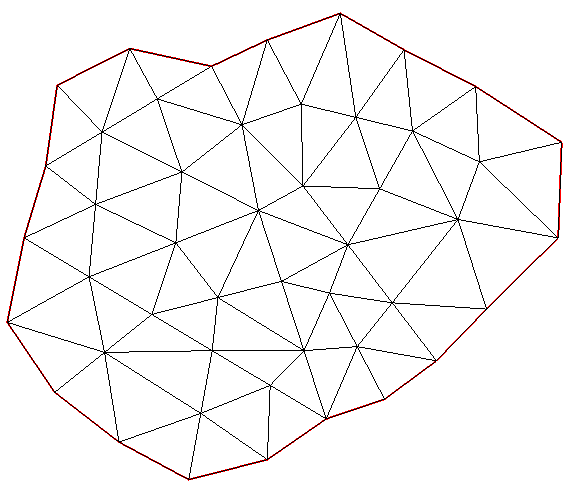
\includegraphics[width=0.4\linewidth]{img/mallaajustadafronteranorefinada}\hfil	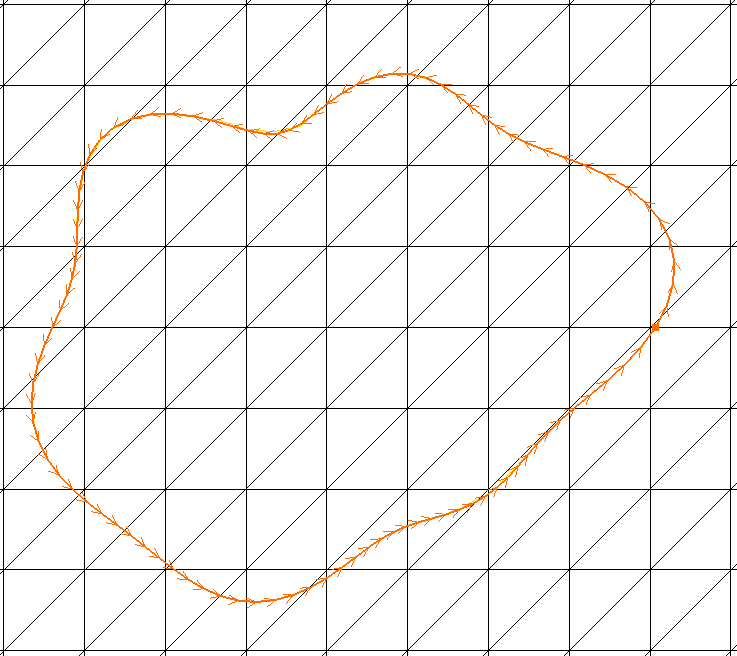
\includegraphics[width=0.4\linewidth]{img/mallanoajustadafrontera}
	\caption{Representación de la frontera. Izquierda: Frontera representada por segmentos rectos. Derecha: Frontera representada por curva de nivel.}
	\label{fig:mallanoajustadafrontera}
\end{figure}
La representación de la frontera ajustada al mallado trae dificultades en el cálculo de la curvatura, además exige que la malla cambie en cada paso de tiempo y por lo tanto la solución numérica debe interpolarse a la nueva malla. La representación por curvas de nivel permite el uso de polinomios de grado 2 y 3, ademas de eliminar la necesidad de cambiar la malla.

Entre los métodos numéricos que utilizan un malla fija y permiten que la frontera o interface cruce los elementos,  se encuentran:
\begin{itemize}
	\item El Método de Elementos Finitos Extendidos (XFEM), basado en enriquecer los elementos interceptados por la interface, con  funciones de forma discontinuas y fue utilizado por primera vez para resolver problemas de propagación de fracturas \citep{olsson2005conservative}. La estabilización se logra desactivando  grados de libertad, por precondicionamiento o mediante el uso de penalidad fantasma.
	\item El Método de Elementos Finitos Cortados (CutFEM)  por otra parte utiliza dominios ficticios en combinación con penalidad fantasma para estabilizar la solución, ha sido utilizado principalmente en problemas de flujos bifásicos \citep{claus2019cutfem}.
	
	\item El Método de Elementos Finitos basado en Conjuntos de Nivel ($\phi$-FEM), presentado en \cite{duprez2020phi}-\cite{cotin2021phifem}  utiliza funciones forma que se anulan en la curva de nivel 0, que representa la frontera, ha sido utilizado en problemas de transferencia de calor y el estudio del	movimiento de partículas rígidas en un fluido regido por las ecuaciones de Stokes.
	\item El Método de Elementos Finitos aplicado a inecuaciones variacionales presentado en \cite{mantilla2003} considera analizar el comportamiento del flujo laminar de un líquido que se filtra a través de una sección transversal de un medio poroso donde la interface entre la región húmeda y la región seca se representa por medio de $q$ una función característica.
	\begin{figure}[H]	
		\centering
		\includegraphics[width=10cm]{img/Zhzsdr.pdf}
		\caption{\label{drsh2b} Filtración en un medio poroso, la frontera que 
			separa la región húmeda y la región seca es representada por una función característica \cite{mantilla2003}.}
	\end{figure}
\end{itemize}
\section{Notaciones}
%Presentamos las siguientes notaciones \citep{brenner2008mathematical}: Sea $\alpha=\left(\alpha_1,\ldots,\alpha_d\right)\in\mathbb{N}^d$  un multi-índice con longitud $|\alpha|=\alpha_1+\cdots +\alpha_d$, entonces $D^\alpha =\left( \partial / \partial x_1\right)^{\alpha_1}\cdots \left( \partial / \partial x_d\right)^{\alpha_d}$. Denotamos por $C^k(\Omega)$ a la clase de funciones en $\Omega$  con derivadas parciales de orden $k$ continuas en $\Omega$, $C_0^k(\Omega)$ denota el conjunto de funciones en $C^k(\Omega)$ con soporte compacto en $\Omega$. Dado $p\in\left [1,+\infty\right>$, $L^p(\Omega)$ denota el espacio de funciones reales $f$ tal que $|f|^p$ es integrable en $\Omega$ respecto a la medida de Lebesgue en $\mathbb{R}^d$. $L^p(\Omega)$ es un espacio de Banach con la norma
%\[
%\|u\|_{L^p(\Omega)} =\left(\int_\Omega |u|^p\right)^{1/p}
%\]
%Ademas $L^2(\Omega)$ es un espacio de Hilbert con el producto interno y norma siguientes
%\[
%\left(u,v\right) = \int_\Omega uv,\quad \|u\|=
%\left(u,u\right)^{1/2}
%\]
%El espacio de funciones con $W^{m,p}(\Omega)$ 
%\[
%\begin{aligned}	
%\|u\|_{m,p} & = \left( \sum_{0\leq|\alpha| \leq m} \| D^\alpha u\|^p_{L^p(\Omega)}\right)^{1/p},\quad 1\leq p <+\infty\\
%\|u\|_{m,\infty} & = \max_{0\leq|\alpha| \leq m} \| D^\alpha u\|_{L^\infty(\Omega)}
%\end{aligned}
%\]
%y las seminormas
%\[
%\begin{aligned}	
%	|u|_{m,p} & = \left( \sum_{|\alpha| = m} \| D^\alpha u\|^p_{L^p(\Omega)}\right)^{1/p},\quad 1\leq p <+\infty\\
%	|u|_{m,\infty} & = \max_{|\alpha| = m} \| D^\alpha u\|_{L^\infty(\Omega)}
%\end{aligned}
%\]
%\end{itemize}
%

Introducimos la notación de multi-índice$\,$para el cálculo de
derivadas parciales. Un multi-índice, $\alpha $, es una d-dupla de
enteros no-negativos, $\alpha _{i}$. La ``longitud'' de $\alpha $ está
dada por $\left| \alpha \right| :=\sum\limits_{i=1}^{d}\alpha _{i}.$ Con
esta notación si $v\in \mathbf{C}^{m}\left( \Omega \right) $ entonces
para cualquier $\alpha $ con $\left| \alpha \right| \leqslant m$,
\[
D^{\alpha }v\left( x\right) =\frac{\partial ^{\left| \alpha \right| }v\left(
	x\right) }{\partial x_{1}^{\alpha _{1}}\cdots\partial x_{d}^{\alpha _{d}}}
\]
es la derivada parcial de $\alpha ^{th}$ orden. Por ejemplo
\[
\frac{\partial v}{\partial x_{1}}=D^{\alpha }v\text{ para }\alpha =\left(
1,0,\ldots,0\right)
\]
\[
\frac{\partial ^{d}v}{\partial x_{1}\cdots\partial x_{d}}=D^{\alpha }v\text{
	para }\alpha =\left( 1,1,\ldots,1\right)
\]

En lo que sigue $\Omega $ designa un conjunto abierto en $\mathbb{R}^{d}$
con frontera $\Gamma $ y se consideran los espacios $\mathbf{L}^{p}\left(
\Omega \right) $, $1\mathbf{\leqslant }p\mathbf{\leqslant }\infty $, dotados
de la medida de Lebesgue $d$-dimensional. $\mathbf{C}_c(\Omega)$ es el espacio de funciones continuas en $\Omega$ con soporte compacto en $\Omega$, es decir se anulan fuera de algún compacto $K\subset \Omega$.

Para un entero $k>0$ definimos los siguientes conjuntos de funciones: $\mathbf{C}_c^k(\Omega)=\mathbf{C}^k(\Omega) \cap \mathbf{C}_c(\Omega)$.
$\mathbf{C}_c^\infty(\Omega)=\mathbf{C}^\infty(\Omega) \cap \mathbf{C}_c(\Omega)$.

\begin{defi}
	Definimos el conjunto $\mathbf{L}_{loc}^{p}(\Omega )$\ para $1\mathbf{%
		\leqslant }p\mathbf{\leqslant }\infty $ y $\Omega \subset \mathbb{R}^{d}%
	\mathit{\ }$como el conjunto de funciones $f$\ tales que:
	\[
	f\in \mathbf{L}^{p}(K)\quad \forall \text{compacto }K\subset \Omega
	\]
\end{defi}

Un ejemplo de función localmente $p$-integrable es
\[
f\left( x\right) =\exp \left( d\left( x,\Gamma \right) ^{-1}\right) \sen%
\left( d\left( x,\Gamma \right) ^{-1}\right)
\]
Así tomando $K\subset \Omega $, $K$ compacto tenemos que existe
$\delta >0$ tal que $d\left( x,\Gamma \right) \geqslant \delta $
para todo $x\in K$ por
tanto $f\left( x\right) $ es continua en $K$ y en consecuencia $p$%
-integrable en $K$. Pero claro $f\left( x\right) \rightarrow +\infty $
cuando $d\left( x,\Gamma \right) \rightarrow 0$.
%\begin{teo}[Urysohn]
%	\label{Teo_Ury}Sea $G\subset \mathbb{R}^{d}$\ un abierto y $K\subset G$\ un
%	conjunto compacto, entonces existe $f\in \mathbf{C}_{c}\left( G\right)$
%	tal que
%	\begin{enumerate}
	%		\item  \hspace{3cm} $0\leqslant f\left( x\right) \leqslant 1\quad\text{
		%			para todo }x\in G$
	%		\item  \hspace{3.5cm} $f\left( x\right) =1\quad\text{para todo }x\in K$
	%	\end{enumerate}
%\end{teo}
%\demo Ver \cite{brez}.\quad\endproof
\begin{teo}[{\cite[p. 109]{brezis2011functional}}]
	\label{CcdensoenL1}El espacio $\mathbf{C}_{c}^{\infty}\left( \Omega \right) $\ es
	denso en $\mathbf{L}^{p}\left( \Omega \right) $, $1\leq p<+\infty$
\end{teo}
\begin{defi}[Derivada débil]
	Decimos que una función $f$\ $\in \mathbf{L}_{loc}^{1}(\Omega )$\ tiene
	derivada débil, $D^{\alpha }f$, cuando exista una función $g\in
	\mathbf{L}_{loc}^{1}(\Omega )$\ tal que
	\[
	\int_{\Omega }g\left( x\right) \phi \left( x\right) \,\mathbf{d}%
	x=(-1)^{\left| \alpha \right| }\int_{\Omega }f\left( x\right)
	D^{\alpha }\phi \left( x\right) \,\mathbf{d}x\qquad \forall \phi \in
	\mathbf{C}_c^\infty(\Omega )
	\]
	y la denotamos por $D^{\alpha }f=g$
\end{defi}
Notemos que si $v\in \mathbf{C}^{m}(\Omega )$, entonces para cada $\alpha $
con $\left| \alpha \right| \leqslant m$, la derivada parcial ``clásica''
coincide con $D^{\alpha }v$. Además la derivada débil está
definida de manera única salvo en un conjunto de medida nula. Usando la
noción de derivada débil, podemos generalizar las normas y espacios
de Lebesgue para que incluyan derivadas.

Una función $v$ es H\"{o}lder continua con exponente $\beta\in \left<0,1 \right]$ si existe $c\in\mathbb{R}$ tal que
\[
|v(x)-v(y)|\leqslant c\|x-y\|^\beta,\quad  \forall x,y\in\Omega
\]
El espacio de  H\"{o}lder $C^{0,\beta}(\overline{\Omega})$ se define como el espacio de funciones continuas en $\overline{\Omega}$ que son H\"{o}lder continuas con exponente $\beta$. Para $m\geq 0$ definimos el espacio de H\"{o}lder $C^{m,\beta}(\overline{\Omega})$,
\[
C^{m,\beta}(\overline{\Omega}) = \left\{
v\in C^m(\overline{\Omega}) | \partial^\alpha v\in C^{0,\beta}(\overline{\Omega}),\forall \alpha:|\alpha|=m
\right\}
\]
\begin{defi}
	Dado $x\in \mathbb{R}^{d}$ escribiremos
	\[
	x=\left( x^{\prime },x_{d}\right) \text{ con }x^{\prime }\in \mathbb{R}%
	^{d-1},\quad x^{\prime }=\left( x_{1},x_{2},\ldots,x_{d-1}\right)
	,\quad x_d\in\mathbb{R}
	\]
	Sea $\Omega \subset \mathbb{R}^{d}$ un abierto acotado y $\mathit{\mathbf{F}}$ un espacio
	de funciones de $\mathbb{R}^{d-1}$ a $\mathbb{R}$. Se dice que $\partial \Omega $ es de clase $%
	\mathit{\mathbf{F}}$, o que $\Omega $ es un dominio $\mathit{\mathbf{F}}$,
	si para todo $x\in \partial \Omega $ existe una vecindad $U$\ de $x$\ en $%
	\mathbb{R}^{d}$\ y una aplicación $H\in \mathbf{F}$ tal que tal que:
	\[
	U\cap \Omega =\left\{ y\in U:y_{d}>H\left( y^{\prime }\right) \right\}
	\]
	Si $\mathbf{F}$  consiste de funciones Lipschitz continuas entonces diremos que $\Omega$ es un dominio Lipschitz. Cuando $\mathbf{F}$ son funciones $C^k$ diremos que $\Omega$ es un dominio $C^k$. Del mismo modo si $\mathbf{F}$ consiste de funciones $C^{k,\alpha}$ diremos que $\partial\Omega$ es una frontera H\"{o}lder de clase $C^{k,\alpha}$.
\end{defi}
\section{Espacios de Sobolev}
\begin{defi}[Espacios de Sobolev de orden entero]
	Sea $k$ un entero no negativo, y sea $v\in \mathbf{L}_{loc}^{1}(\Omega )
	$. Supongamos que $D^{\alpha }v$ exista para todo $\left| \alpha \right|
	\mathbf{\leqslant }k$. Definimos entonces la norma de Sobolev como:
	\[
	\left\| v\right\| _{\mathbf{W}_{p}^{k}(\Omega )}=\left( \sum_{\left|
		\alpha \right| \mathbf{\leqslant }k}\left\| D^{\alpha }v\right\| _{\mathbf{L}%
		^{p}(\Omega )}^{p}\right) ^{1/p}
	\]
	en el caso $1\leqslant p<\infty$, y como
	\[
	\left\| v\right\| _{\mathbf{W}_{\infty }^{k}(\Omega )}=\max\limits_{\left|
		\alpha \right| \mathbf{\leqslant }k}\left\| D^{\alpha }v\right\| _{\mathbf{L}%
		^{\infty }(\Omega )}
	\]
	en el caso $p=\infty $
	
	En cada caso, definimos los espacios de Sobolev como
	\[
	\mathbf{W}_{p}^{k}(\Omega )=\left\{ v\in \mathbf{L}_{loc}^{1}(\Omega
	):\left\| v\right\| _{\mathbf{W}_{p}^{k}(\Omega )}<\infty \right\} .
	\]
\end{defi}

También definimos una seminorma en $\mathbf{W}_{p}^{k}(\Omega )$ como
\[
\left| v\right| _{\mathbf{W}_{p}^{k}(\Omega )}:=\left\{
\begin{array}[c]{cl}
	\left( \displaystyle \sum_{\left| \alpha \right| =k}\left\| D^{\alpha }v\right\| _{%
		\mathbf{L}^{p}(\Omega )}^{p}\right) ^{1/p} & :1\leqslant p<\infty
	\\
	\max\limits_{\left| \alpha \right| =k}\left\| D^{\alpha }v\right\| _{\mathbf{%
			L}^{\infty }(\Omega )} & :p=\infty
\end{array}
\right.
\]
En los sucesivo denotaremos $\mathbf{W}^{k,2}(\Omega )$ como $\mathbf{H}%
^{k}(\Omega )$, que son los espacios en que comúnmente se analizan los
operadores diferenciales.

\begin{teo}[{\cite[p. 285]{han2009theoretical}}]
	Los espacios de Sobolev $\mathbf{W}^{k,p}(\Omega )$\ son espacios de Banach
	y por tanto los espacios $\mathbf{H}^{k}(\Omega )$\ son espacios de Hilbert
	con el producto interno
	\[
	\left( u,v\right) _{\mathbf{H}^{k}}=\int_{\Omega
	}\sum_{\left| \alpha \right| \mathbf{\leqslant }k}D^{\alpha }u\left(
	x\right) D^{\alpha }v\left( x\right) \,\mathbf{d}x\quad \forall u,v\in
	\mathbf{H}^{k}(\Omega )
	\]
\end{teo}

\begin{obs}[{\cite[p. 271]{brezis2011functional}}]
	Si $\Omega $\ es suficientemente regular entonces la norma $\mathbf{W}%
	_{p}^{k}(\Omega )$\ es equivalente a la norma
	\[
	\left\| u\right\| _{\mathbf{L}^{p}(\Omega )}+\sum_{\left| \alpha
		\right| =k}\left\| D^{\alpha }u\right\| _{\mathbf{L}^{p}(\Omega )}
	\]
\end{obs}
Los siguientes son teoremas de densidad que nos permiten aproximar
funciones en espacios de Sobolev por funciones suficientemente
suaves bajo algunas condiciones respecto a la región $\Omega $

\begin{teo}[{\cite[p. 294]{han2009theoretical}}]
	Si $v\in \mathbf{W}^{k,p}\left( \Omega \right) $, con $1\leqslant p<+\infty $
	entonces existe una sucesión $\left\{ v_{n}\right\} \subset \mathbf{C}^{\infty
	}\left( \Omega \right) \cap \mathbf{W}^{k,p}\left( \Omega \right) $ tal que
	\[
	\lim_{n\rightarrow \infty }\left\| v_{n}-v\right\| _{\mathbf{W}^{k,p}}=0
	\]
\end{teo}
\begin{teo}[{\cite[p. 294]{han2009theoretical}}]
	Si $v\in \mathbf{W}^{k,p}\left( \Omega \right)$, $1\leqslant p<+\infty $ y
	además $\Omega $ es un dominio Lipschitz, entonces existe una
	sucesión $\left\{ v_{n}\right\} \subset \mathbf{C}^{\infty }\left(
	\overline{\Omega }\right) $ tal que
	\[
	\lim_{n\rightarrow \infty }\left\| v_{n}-v\right\| _{\mathbf{W}^{k,p}}=0
	\]
\end{teo}
%
%\begin{teo}[{\cite[p. 294]{brezis2011functional}}]
%	Si $v\in \mathbf{W}^{1,p}\left( \Omega \right)$, $1\leqslant p<+\infty $ y
%	además $\Omega $ es de clase $\mathbf{C}^{1}$, entonces existe una
%	sucesión $\left\{ v_{n}\right\} \subset \mathbf{C}_{c}^{\infty }\left( %
%	\mathbb{R}^{d}\right) $ tal que $v_{n}\mid _{\Omega }\rightarrow v$ en $%
%	\mathbf{W}^{1,p}\left( \Omega \right) $.
%\end{teo}
%\demo Ver \cite{brez}.\endproof
\begin{teo}[{\cite[p. 294]{han2009theoretical}}]
	Si $k\geqslant 0$ y $1\leqslant p<+\infty $; entonces $\mathbf{C}_{c}^{\infty }(\mathbb{R}%
	^{d})$ es denso en $\mathbf{W}^{k,p}\left( \mathbb{R}%
	^{d} \right) $.
\end{teo}

\begin{teo}[{\cite[p. 295]{han2009theoretical}}]
	\label{teo_desi_sobolev}Suponemos $\Omega \subset \mathbb{R}^{d}$ un
	dominio Lipschitz, entonces para $k\geqslant 1$ y
	$1\leqslant p<\infty$:
	\[
	\begin{array}[c]{ccll}
		\textrm{si} & \frac{1}{p}-\frac{k}{d}>0, & \textrm{tenemos que} & \mathbf{W}%
		^{k,p}\left( \Omega \right) \subset \mathbf{L}^{q}\left( \Omega \right)
		\textrm{\qquad }\forall q\leqslant p^{*},\frac{1}{p^{*}}=\frac{1}{p}-\frac{k}{d%
		}, \\
		\textrm{si} & \frac{1}{p}-\frac{k}{d}=0, & \textrm{tenemos que} & \mathbf{W}%
		^{k,p}\left( \Omega \right) \subset \mathbf{L}^{q}\left( \Omega \right)
		\textrm{\qquad }\forall q<+\infty , \\
		\textrm{si} & \frac{1}{p}-\frac{k}{d}<0, & \textrm{tenemos que} & \mathbf{W}%
		^{k,p}\left( \Omega \right) \subset \mathbf{C}^{k-\llbracket \frac{d}{p}\rrbracket -1,\beta}\left( \Omega
		\right) \textrm{\qquad con } \beta =\begin{cases}
			\llbracket \frac{d}{p}\rrbracket +1-\frac{d}{p}, &
			\text{ si }\frac{d}{p}\not\in\mathbb{Z},\\
			\in \left<0,1\right>,&\text{ si } \frac{d}{p}\in\mathbb{Z}.\\
		\end{cases}
	\end{array}
	\]
\end{teo}

\begin{obs}
	El Teorema \ref{teo_desi_sobolev} implica la existencia de una
	función continua $\tilde{u}$, tal que $u=\tilde{u}$ c.t.p. en $%
	\overline{\Omega }$.
	
	Es decir toda función $u\in \mathbf{W}^{k,p}\left( \Omega\right)
	$, $k>\frac{d}{p}$\ admite un representante de clase $\mathbf{C}^{\llbracket k-%
		\frac{d}{p}\rrbracket }\left( \overline{\Omega }\right) $, esto es %
	importante cuando se trata con funciones de $\mathbf{H}^{2}\left( \Omega \right)$ con
	$\Omega \subset \mathbb{R}^{2}$ ya que utilizando el teorema anterior
	con $k=2$, $p=2$\ y $d=2$;\ se tiene que $k-\frac{d}{p}=1$ y por tanto
	obtenemos que $\mathbf{H}^{2}\left( \Omega \right) \subset \mathbf{C}%
	^{1}\left( \overline{\Omega }\right) $ lo que permite usar las propiedades
	conocidas de las funciones continuas.
\end{obs}
\begin{defi}
	Se define como la cerradura de $\mathcal{D}\left( \Omega \right) $\ en $%
	\mathbf{W}^{k,p}\left( \Omega \right) $, al espacio funcional $\mathbf{W}%
	_{0}^{k,p}\left( \Omega \right) $, para $1\leqslant p<\infty $.$\mathit{\ }$%
	En particular para $p=2$
	\[
	\mathbf{H}_{0}^{k}\left( \Omega \right) \equiv \mathbf{W}_{0}^{k,2}\left(
	\Omega \right)
	\]
\end{defi}
\begin{teo}[Desigualdad de Poincaré{\cite[p. 290]{brezis2011functional}}]	
	\label{teo_poincare}Suponemos $\Omega $\ un abierto acotado en al menos una
	dirección. Entonces existe una constante $C$\ (dependiendo sólo de $%
	\Omega $\ y $p$) tal que
	\[
	\left\| u\right\| _{\mathbf{L}^{p}}\leqslant C\left\| \nabla u\right\| _{%
		\mathbf{L}^{p}}\qquad \forall u\in \mathbf{W}_{0}^{1,p}\left( \Omega \right)
	\quad \left( 1\leqslant p<\infty \right) .
	\]
	En particular la expresión $\left\| \nabla u\right\| _{\mathbf{L}^{p}}$\
	es una norma de $\mathbf{W}_{0}^{1,p}\left( \Omega \right) $\ equivalente a
	la norma $\left\| u\right\| _{\mathbf{W}^{1,p}}$ del espacio $\mathbf{H}%
	_{0}^{1}\left( \Omega \right) $.
	
	La expresión $\int_{\Omega }\nabla u\cdot \nabla v$\ es un producto
	interno que induce a la norma $\left\| \nabla u\right\| _{\mathbf{L}^{2}}$\
	equivalente a $\left\| u\right\| _{\mathbf{H}^{1}}$
\end{teo}

\begin{defi}[Espacios de Sobolev de orden real]
	Sea $s=k+\delta $\ con $k\geqslant 0$\ y $\delta \in \left] 0,1\right[ $\ .
	Definimos el espacio de Sobolev de orden real positivo para $p\in \left[
	0,\infty \right[ $\ como
	\[
	\mathbf{W}_{p}^{s}(\Omega ):=\left\{ v\in \mathbf{W}_{p}^{k}(\Omega ):\frac{%
		\left| D^{\alpha }v\left( x\right) -D^{\alpha }v\left( y\right) \right| }{%
		\left\| x-y\right\| ^{\delta +\frac{\mathbf{N}}{p}}}\in \mathbf{L}%
	^{p}(\Omega \times \Omega ):\forall \alpha :\left| \alpha \right| =k\right\}
	\]
	dotado de la norma
	\[
	\left\| v\right\| _{\mathbf{W}_{p}^{s}(\Omega )}=\left\{ \left\| v\right\| _{%
		\mathbf{W}_{p}^{k}(\Omega )}^{p}+\sum_{\left| \alpha \right|
		=m}\,\,\int_{\Omega \times \Omega }\frac{\left| D^{\alpha }v\left(
		x\right) -D^{\alpha }v\left( y\right) \right| ^{p}}{\left\| x-y\right\|
		^{\delta p+\mathbf{N}}}\mathbf{d}x\mathbf{d}y\right\} ^{\frac{1}{p}}.
	\]
\end{defi}
\begin{defi}[Espacios de Sobolev de orden negativo]
	Sean $s\geqslant 0$\ real, $p\in \left] 1,\infty \right[ $\ y $p^{\prime }$\
	(exponente conjugado de $p$)\ tales que $\frac{1}{p}+\frac{1}{p^{\prime }}=1$%
	, se define como el dual de $\mathbf{W}^{s,p}\left( \Omega \right) $\ al
	espacio funcional de orden negativo $\mathbf{W}^{-s,p^{\prime }}(\Omega )$.
	
	En particular para $p=2$, el dual de $\mathbf{W}^{s,2}(\Omega )$ está
	definido por $\mathbf{W}^{-s,2}(\Omega )$\ tal que
	\[
	\mathbf{H}^{-s}(\Omega )\equiv \mathbf{W}^{-s,2}(\Omega ).
	\]
\end{defi}
Los siguientes teoremas nos permiten estudiar el comportamiento de las
funciones que admiten derivada débil en la frontera de $\Omega $.
\begin{teo}	[{\cite[p. 297]{han2009theoretical}}]
	\label{Teorema de Trazas}Sea $\Omega $\ un conjunto abierto, acotado y de
	Lipschitz. Entonces existe un operador lineal continuo $\gamma _{0}:\mathbf{W%
	}^{1,p}\left( \Omega \right) \rightarrow \mathbf{L}^{p}\left( \Gamma \right)
	$, $1\leqslant p<\infty $, tal que:
	\begin{enumerate}
		\item  $\gamma _{0}v=v\mid _{\Gamma }$\ si $v\in \mathbf{W}^{1,p}\left(
		\Omega \right) \cap \mathbf{C}\left( \overline{\Omega }\right) .$
		\item  Existe $c_{1}>0,$\ de manera que:
		\[
		\left\| \gamma _{0}v\right\| _{\mathbf{L}^{p}(\Gamma )}\leqslant
		c_{1}\left\| v\right\| _{\mathbf{W}^{1,p}(\Omega )}\qquad \forall v\in
		\mathbf{W}^{1,p}(\Omega )
		\]
		\item  Existe $c_{2}>0,$\ de manera que:
		\[
		\left\| \gamma _{0}v\right\| _{\mathbf{W}^{1-1/p,p}(\Gamma )}\leqslant
		c_{2}\left\| v\right\| _{\mathbf{W}^{1,p}(\Omega )}\qquad \forall v\in
		\mathbf{W}^{1,p}(\Omega )
		\]
		además el operador traza $\gamma _{0}$\ es sobreyectivo, es decir $%
		\gamma _{0}\left( \mathbf{W}^{1,p}(\Omega )\right) =\mathbf{W}%
		^{1-1/p,p}(\Gamma )$
		\item  El núcleo del operador traza es $\mathbf{W}_{0}^{1,p}(\Omega )$,
		es decir
		\[
		\mathbf{W}_{0}^{1,p}(\Omega )=\left\{ v\in \mathbf{W}^{1,p}(\Omega ):\gamma
		_{0}v=0\right\}
		\]
		\item  La aplicación $\gamma _{0}:\mathbf{W}^{1,p}\left( \Omega \right)
		\rightarrow \mathbf{L}^{p}\left( \Gamma \right) $\ es compacta, es decir
		para cualquier sucesión acotada $\left\{ v_{n}\right\} $\ en $\mathbf{W}%
		^{1,p}\left( \Omega \right) $, existe una subsucesión $\left\{
		v_{n}^{\prime }\right\} \subset \left\{ v_{n}\right\} $\ tal que $\left\{
		\gamma _{0}v_{n}^{\prime }\right\} $\ es convergente $\mathbf{L}^{p}\left(
		\Gamma \right) $
	\end{enumerate}
	De igual modo asumamos $\Omega $\ un conjunto abierto y acotado de clase $%
	\mathbf{C}^{1,1}$\ con frontera $\Gamma $. Si $1\leqslant p<\infty $\ y $m>1+%
	\frac{1}{p}$. Entonces existen únicos operadores lineales continuos y
	sobreyectivos $\gamma _{0}:\mathbf{W}^{m,p}\left( \Omega \right) \rightarrow
	\mathbf{W}^{m-\frac{1}{p},p}\left( \Gamma \right)$ y $\gamma _{1}:\mathbf{W}%
	^{m,p}\left( \Omega \right) \rightarrow \mathbf{W}^{m-1-\frac{1}{p},p}\left(
	\Gamma \right) $ tal que $\gamma _{0}v=\left.v\right\vert_{\Gamma }$ y $\gamma
	_{1}v=\left. \frac{\partial v}{\partial n}\right\vert_{\Gamma }$ si $v\in
	\mathbf{W}^{m,p}\left( \Omega \right) \cap \mathbf{C}^{1}\left( \overline{%
		\Omega }\right) $
\end{teo}

\begin{teo}[Fórmulas de Green{\cite[p. 323]{han2009theoretical}}]	
	Sea $\Omega \subset \mathbb{R}^{d}$\ un dominio Lipschitz abierto y acotado.
	Entonces
	\[
	\int_{\Omega }\frac{\partial u}{\partial x_{i}}v\,\mathbf{d}%
	x=-\int_{\Omega }u\frac{\partial v}{\partial x_{i}}\,\mathbf{d}%
	\Gamma +\int_{\Gamma }uvn_{i}\,\mathbf{d}\Gamma \quad \forall u,v\in
	\mathbf{H}^{1}(\Omega )
	\]
	donde $n=\left( n_{1},...,n_{d}\right) $\ es el vector normal unitario
	exterior a $\Gamma $.\ También\ se tiene
	\[
	-\int_{\Omega }\Delta u\,v\,\mathbf{d}x=\int_{\Omega }\nabla
	u\cdot \nabla v\,\mathbf{d}x-\int_{\Gamma }\frac{%
		\partial u}{\partial n}v\,\mathbf{d}\Gamma \quad \forall u\in \mathbf{H}%
	^{2}(\Omega ),v\in \mathbf{H}^{1}(\Omega )
	\]
	y
	\[
	\int_{\Omega }\left( \nabla\cdot\mathbf{u}\right) \,v\,\mathbf{d}%
	x=-\int_{\Omega }\mathbf{u}\cdot \nabla v\,\mathbf{d}%
	x+\int_{\Gamma }\left( \mathbf{u}\cdot n\right) v\,\mathbf{d}\Gamma
	\quad \forall \mathbf{u}\in \left( \mathbf{H}^{1}(\Omega )\right) ^{d},v\in
	\mathbf{H}^{1}(\Omega )
	\]
	para $\mathbf{u}=\left( u_{1},...,u_{d}\right) $\ y donde  la divergencia de $\mathbf{u}$ es
	\[
	\nabla\cdot\mathbf{u}=\sum_{i=1}^{d}\frac{\partial u_{i}}{%
		\partial x_{i}}
	\]
\end{teo}


%@book{brezis2011functional,
	%@book{han2009theoretical

\chapter{\MakeUppercase{Planteamiento del problema dinámico del tumor avascular}}
%\chapter{Planteamiento del problema dinámico del tumor avascular}
\thispagestyle{fancy}
\section{Planteamiento del modelo matemático del crecimiento dinámico tumoral}
Consideramos que el tumor ocupa un dominio acotado $\Omega\subset\mathbb{R}^2$ con frontera $\Gamma$  que cambia con el tiempo $t$ medido en minutos. Las variables de la dinámica del crecimiento tumoral son la concentración de nutrientes y la presión intracelular.

La concentración de nutrientes al interior del tumor se representa mediante la función $\sigma$ $\equiv$ $\sigma(x,y,t)$ que obedece a la siguiente ecuación de difusión:
\begin{equation}
	D_N \Delta \sigma - \gamma (\sigma -\sigma_B )-\delta_N \sigma=0 \text{ en } \Omega
\end{equation}
donde $D_N$ es el coeficiente de difusión, $- \gamma (\sigma -\sigma_B )$ modela la velocidad de transferencia de nutrientes desde los vasos sanguíneos,  $\delta_N \sigma$ representa el consumo de nutrientes  por parte de la células vivas en el tumor. 

Adicionalmente el tumor es modelado como un fluido incompresible de velocidad $u\equiv u(x,y,t)$ que se rige por la ecuación de continuidad
\begin{equation}
	\nabla \cdot u = \gamma_T \sigma - \delta _T\text{ en } \Omega
\end{equation}
donde el lado derecho de la ecuación expresa la velocidad de reproducción  de las células del tumor menos la velocidad de muerte celular.

La velocidad está relacionada con el gradiente de presión por medio de la ley de Darcy:
\begin{equation}
	u=-w_t \nabla p \text{ en } \Omega
\end{equation}
donde $p\equiv p(x,y,t)$ es la presión del fluido al interior del tumor y $w_T$ representa la movilidad celular, lo que nos permite escribir la siguiente ecuación para la presión 
\begin{equation}
	\Delta p = -\frac{\gamma_T}{w_T} \sigma + \frac{\delta _T}{w_T}\text{ en } \Omega
\end{equation}

\section{Condiciones de borde en la frontera libre}
Asumimos que la concentración de nutrientes $\sigma_{out}$ en la frontera del tumor es constante e igual a la concentración de nutriente en el exterior del tumor.
\begin{equation}
	\sigma |_{\Gamma}  = \sigma_{out}
\end{equation}

La presión satisface la relación de Young-Laplace en la frontera 
\begin{equation}
	p |_{\Gamma}  = \gamma \kappa
\end{equation}
donde $\gamma$ representa la tensión superficial y $\kappa$ es la curvatura de la frontera $\partial\Omega$.

La velocidad normal $V_n$, con la que se desplaza la frontera del tumor es la componente normal de la velocidad $u$ 
\begin{equation}
	V_n = 	u |_{\Gamma} \cdot n  = 
	-w_T	\nabla p |_{\Gamma} \cdot n 
\end{equation}
donde $n$ es la normal unitaria exterior a $\Gamma$.

\section{Modelo adimensional}

Siguiendo \citep{cristini2008nonlinear} introducimos las siguientes constantes
\begin{align}
	L_D & = \dfrac{ D_N^{1/2}}{ (\gamma_B + \delta_N)^{1/2}}\\
	\lambda_R &= \frac{w_T \gamma}{ L^3_D}
\end{align}
y variables adimensionales
\begin{align}
	\overline{x} & = \dfrac{ x}{L_D}\\
	\overline{y} & = \dfrac{ y}{L_D}\\
	\overline{t} & = \lambda_R t\\	
	\overline{\sigma} & = \dfrac{ \sigma}{\sigma_{out}}\\
	\overline{p} & = \dfrac{ L_D}{\gamma }p					
\end{align}
Así el modelo de crecimiento tumoral queda expresado en las siguientes ecuaciones adimensionales:
\begin{align}
	&	\Delta \overline{\sigma}- \overline{\sigma}+  \frac{\gamma_B\sigma_B}{\sigma_{out}(\gamma_B + \delta_N)}=0 \text{ en } \overline{\Omega}\\
	&	\Delta \overline{p} = -\frac{\gamma_T \sigma_{out}}{\lambda_R} \overline{\sigma} + \frac{\delta _T}{\lambda_R}\text{ en } \overline{\Omega}\\
	&	\overline{\sigma} |_{\partial \overline{\Omega}}  = 1\\
	&	\overline{p} |_{\partial \overline{\Omega}}  = \kappa \\
	&	\overline{V}_n = 	
	-	\nabla \overline{p} |_{\partial \overline{\Omega}} \cdot n 
\end{align}
donde $\overline{\Omega}$ es el dominio luego del cambio de coordenadas con las variables adimensionales $(\overline{x},\overline{y})$.
\section{Modelo desacoplado}
El modelo acoplado anterior puede simplificarse si hacemos 
\begin{equation}
	\lambda_M= \gamma_T \sigma_{out}
\end{equation}
\begin{equation}
	B=\frac{\gamma_B\sigma_B}{\sigma_{out}(\gamma_B + \delta_N)}
\end{equation}
\begin{equation} 
	G=\frac{\lambda_M}{\lambda_R}(1-B)
	\label{eqn:G}
\end{equation}
\begin{equation}
	A=\frac{\dfrac{\delta_T}{\lambda_M}-B}{1-B}
	\label{eqn:A}
\end{equation}
\begin{equation}
	U=\frac{ \overline{\sigma}-B }{1-B}
\end{equation}
\begin{equation}
	P=\overline{p} + (1-U)G- AG\left( \frac{\overline{x}^2+\overline{y}^2}{4}\right)
\end{equation}
de modo que las nuevas variables $U$, $P$, $V_n$ satisfacen el siguiente sistema de ecuaciones:
\begin{align}
	-\Delta U + U  &= 0 \text{ en }  \overline{\Omega}\\
	U &= 1 	 \text{ en }  \partial \overline{\Omega}\\
	\Delta P  &= 0 \text{ en }  \overline{\Omega}\\
	P &= \kappa - AG\left( \frac{\overline{x}^2+\overline{y}^2}{4} \right)	 \text{ en }  \partial \overline{\Omega}\\
	V_n& =-\nabla P \cdot n + G \nabla U \cdot n- AG \frac{n\cdot (\overline{x},\overline{y})}{2} \text{ en }  \partial \overline{\Omega} \label{eqn:velocidadVn}
\end{align}	
Para simplificar la notación se omitirán  barras al escribir los dominios y cantidades relacionadas a las variables adimensionales.

\section{Evolución de la frontera libre}
Consideramos que $\Omega$ y $\Gamma$ pueden ser definidas mediante cierta función $\phi$ llamada también \emph{función conjunto de nivel}:
\[
\Omega = \{ \phi<0\}\quad y \quad  \Gamma
=\{ \phi =0\}.
\]
además suponemos que $\phi$ en $t=0$ se comporta como una función distancia dirigida 
\[
\phi(x)=
\left\{
\begin{aligned}
	-{\rm dist}(x,\Gamma)&,&x\in\Omega\\
	{\rm dist}(x,\Gamma)&,&x\not\in\Omega
\end{aligned}
\right.
\]
en tal caso $\phi$ es Lipschitz continua, y si es diferenciable en $x\not \in \Gamma$ entonces $|\nabla \phi|=1$ \citep{delfour1994shape}. Como $\Gamma$ es una  curva de nivel 0 para $\phi$ entonces la normal exterior a $\Gamma$ es
\[
n = \frac{\nabla \phi}{|\nabla \phi|}
\]

Por ejemplo, para $\Omega=\{(x,y):x^2+y^2<R^2\}$ podemos elegir $\phi(x,y)=\sqrt{x^2+y^2}-R$ y en consecuencia  $\nabla\phi=(x/\sqrt{x^2+y^2},y/\sqrt{x^2+y^2})$ excepto en el origen, y la normal unitaria es $n=(x/R,y/R)$ en $\Gamma$.

En términos de las curvas de nivel, la curvatura está dada por
\[
\kappa = \nabla \cdot n = 
\nabla \cdot \left(\frac{\nabla \phi }{ |\nabla \phi |} \right)
=\frac{ \phi_{xx} \phi_{y}^2 - 2 \phi_{x} \phi_{y} \phi_{xy}
	+\phi_{yy} \phi_{x}^2  }{  ( \phi_{x}^2+ \phi_{y}^2   )^{1/2}}
\] 
de igual manera si $\Gamma$ se puede representar en forma polar $\left\{ (r,\theta),r\geq 0,r=f(\theta) \right\}$ entonces la función conjunto de nivel será $\phi(r,\theta) = r-f(\theta)$ y la curvatura está dada por
\[
\kappa =\frac{r^2 +2(f'(\theta))^2-rf''(\theta)}{
	\left[
	(f'(\theta))^2+r^2
	\right]^{3/2}
}
\]
y $
\nabla \phi =(\cos\theta,\sen\theta)+\frac{f'(\theta)}{r}(\sen\theta,-\cos\theta)$ de modo que $|\nabla \phi|=\sqrt{1+\frac{f'(\theta)^2}{r^2}}$.

En cualquier instante $t$ la frontera del tumor $\Gamma(t)$ está dada por el conjunto de nivel 0,
\[
\Gamma(t) =\left\{ (x,y): \phi(x,y,t)=0\right\}
\] y si una partícula permanece en la  posición $(x(t),y(t))$ sobre la frontera, entonces  $\phi(x(t),y(t),t)=0$, por lo tanto
\[
\begin{aligned}	
	\frac{d \phi}{dt}=0&= \frac{\partial \phi}{ \partial t}
	+\frac{\partial \phi}{ \partial x} \frac{d x}{dt}
	+\frac{\partial \phi}{ \partial y} \frac{d y}{dt}\\
	&=\frac{\partial \phi}{ \partial t}+\nabla \phi \cdot V
\end{aligned}
\]
donde $V$ es la velocidad de la partícula. Como 
la normal unitaria en la frontera está dada por $
n = \frac{\nabla \phi}{|\nabla \phi|}$ y $V=V_n n$  entonces
\[
\begin{aligned}	
	\frac{\partial \phi}{ \partial t}+V_n |\nabla \phi |=0\text{ en } \Gamma(t)
\end{aligned}
\]
esta ecuación solo es válida en la frontera, sin embargo al introducir la función conjunto de nivel podemos resolver la ecuación en un dominio fijo $\mathcal{O}\subset \mathbb{R}^{2}$, para ello es necesario encontrar una extensión $S=(S_1, S_2)$ para la velocidad $V$ de tal modo que 
\[
S_1 = V_n n_1, S_2 = V_n n_2\text{ en }\Gamma
\]
y así plantear la siguiente ecuación de advección para $\phi$
\begin{equation}
	\frac{\partial \phi}{ \partial t} + S \cdot \nabla \phi=0\text{ en } \mathcal{O}
	\label{eqn:evolucionconjuntodenivel}
\end{equation}
\section{Extensión de la velocidad de crecimiento}
Decimos que $u_{ext}$ es la extensión de $u_0$ definida en $\Gamma$ a todo el dominio fijo $\mathcal{O}$ si es la solución del siguiente problema:
\begin{equation}
	\begin{cases}
		\nabla \phi \cdot \nabla u =0& \text{ en }\mathcal{O}\\
		u =u_0 &\text{ en }\Gamma
	\end{cases}	
	\label{eqn:extension}
\end{equation}
Sea $S=(S_1, S_2)$ una extensión de la velocidad $V=(v_1,v_2)$ en la frontera del tumor, de modo que $S_1$ extiende $v_1$ y $S_2$ extiende $v_2$, es decir  $\nabla S_1 \cdot \nabla\phi =0$ y $\nabla S_2 \cdot \nabla\phi =0$ por lo tanto
\[
(S_1)_x \phi_x +(S_1)_y \phi_y=0
\]
\[
(S_2)_x \phi_x +(S_2)_y \phi_y=0
\]
Derivamos la expresión dada en la ecuación \ref{eqn:evolucionconjuntodenivel} respecto de $x$
\[
\frac{ \partial\phi_x}{ \partial t} + S_1 \phi_{xx}  + S_2 \phi_{xy}  +  (S_1)_x \phi_{x}  + (S_2)_x \phi_{y} =0
\]
 y también respecto de $y$ 
\[
\frac{\partial \phi_y}{ \partial t} + S_1 \phi_{xy}  + S_2 \phi_{yy}  +  (S_1)_y \phi_{x}  + (S_2)_y \phi_{y} =0
\]
multiplicamos por $\phi_x$, $\phi_y$ respectivamente y sumamos
\[
\frac{\partial |\nabla \phi|^2}{ \partial t} + 
\phi_x(\nabla S_1 \cdot \nabla\phi ) + \phi_y(\nabla S_2 \cdot \nabla\phi )
+ \frac{1}{2} S\cdot \nabla (\|\nabla \phi\|^2)=0
\]
de modo que si $\|\nabla \phi\|^2=1$ entonces $\frac{\partial |\nabla \phi|^2}{ \partial t}=0$, es decir la propiedad de la distancia dirigida es conservada.

\begin{defi}
Sea $F$ una función de $V$ en $\mathbb{R}$. Si existe
\[
\lim_{t\to 0^+} \frac{F(u+tv)-F(u)}{t}
\]
entonces será llamado derivada direccional de $F$ en la dirección $v$ y denotado por $F'(u;v)$. Si $F'(u;v)$ existe para todo $v\in V$ entonces $F$ se dice G\^{a}teaux diferenciable en $u$ y la aplicación lineal $\partial F[u]:V\to\mathbb{R}$ tal que $\partial F[u](v)=F'(u;v)$ se llama derivada de G\^{a}teaux de $F$ en $u$.
\end{defi}

Para formular la ecuación \ref{eqn:extension} como un problema elíptico definimos 
\[
R(v)= \frac{1}{2}\int_\mathcal{O} (\nabla \phi \cdot \nabla v)^2 + \frac{\gamma}{2}\int_\Gamma (v-u_0)^2
\] de modo que si $u$ extiende $u_0$ entonces de acuerdo a \citep{utz2018high}  se resuelve el  siguiente problema de minimización: 
\[
\min_{v\in H^1(\mathcal{O})} R(v) 
\]
luego la derivada de G\^{a}teaux es
\[
\partial R[u](v)=\lim_{t\to 0}\frac{R(u+tv)-R(u)}{t} = \int_\mathcal{O} (\nabla \phi \cdot \nabla u)(\nabla \phi \cdot \nabla v)+
\gamma \int_\Gamma (u-u_0)v
\]
formalmente podemos multiplicar por $\nabla \phi \cdot \nabla v$ y luego 
\[
\int_\mathcal{O} (\nabla \phi \cdot \nabla u)(\nabla \phi \cdot \nabla v)=-\int_\mathcal{O}( \nabla \cdot (A \nabla u))v+\int_{\partial\mathcal{O}}    ((A \nabla u) \cdot n)v
\]
donde $A=\begin{bmatrix} \phi_x^2 &  \phi_{x}\phi_{y} \\ \phi_{x}\phi_{y} & \phi_y^2 \end{bmatrix}$, lo que nos lleva al siguiente problema elíptico
\begin{equation}
	\begin{aligned}
		\nabla \cdot (A \nabla u)=0 & \text{ en }  \mathcal{O}\setminus \Gamma \\
		(A \nabla u) \cdot n=0 &	 \text{ en }  \partial \mathcal{O}\\
		u=u_0 &	 \text{ en } \Gamma
	\end{aligned}
\end{equation}
que debe resolverse para encontrar $S_1$ y $S_2$.


\section{Solución circular}
Recordemos que la ecuación 
\[
-\Delta u + \beta u =0
\]
es equivalente en coordenadas polares a
\[
u_{rr}+\frac{1}{r^2}u_{\theta\theta}+\frac{1}{r}u_r-\beta u=0
\]
si consideramos el caso de las soluciones con  simetría radial, es decir $u_{\theta}=0$, y $\partial\Omega=\left\{(r;\theta): r=R\right\}$  entonces $\kappa=1/R$, por lo tanto la ecuación para la presión se reduce a:
\[
\begin{aligned}
	P''(r)+\frac{1}{r}P'(r) &= 0 \text{ en }  \left]0,R\right[\\
	P(R) &= \frac{1}{R} - AG \frac{R}{4}  \\
\end{aligned}
\]	
cuya solución no singular es constante: $P(r) = \frac{1}{R} - AG \frac{R}{4},r\in[0,R]$.

La ecuación para la concentración de nutrientes se reduce a la ecuación diferencial de segundo orden del tipo
\begin{equation}
	\begin{aligned}
		r^2 U''(r)+rU'(r)-r^2U(r)&= 0 \text{ en }  \left]0,R\right[\\
		U(R) &= 1\\
	\end{aligned}
	\label{eqn:edocircular}
\end{equation}
que tiene como solución no singular  $U(r)=\frac{I_0(r)}{I_0(R)},r\in[0,R]$, donde $I_0(x)$ es una función modificada de Bessel de primer tipo \citep{gradshteyn2014table} cuya forma explícita es: 
\[
I_p(x)=\left( \frac{x}{2} \right)^p \sum_{k=0}^\infty \frac{x^{2k}}{4^k k!\Gamma(p+k+1)},x\in\mathbb{R},p>-1
\]
en particular
\[
I_0(x)=\sum_{k=0}^\infty \frac{(\frac{1}{4}x^2)^k}{(k!)^2}
\]
luego la velocidad de crecimiento del radio del tumor $R$, será
\begin{equation}
	\begin{aligned}
		V=\frac{dR}{dt}&=G\nabla U\cdot n-AG\frac{n\cdot(x,y)}{2}\\
		&=GU'(R)-AG\frac{R}{2}\\
		&=G\frac{I_1(R)}{I_0(R)}-AG\frac{R}{2}	
	\end{aligned}
	\label{eqn:edoradiotumor}
\end{equation}
De \citep{simpson1984some} vemos que $w_0:\left]0,+\infty\right[\to\mathbb{R}$ definida por $w_0(x)=\dfrac{xI_0(x)}{I_1(x)}$ es estrictamente creciente y convexa, %además de \citep{baricz2010bounds} tenemos que
%\[
%\frac{I_1(x)}{xI_0(x)}=\sum_{n\geq 1}\frac{2}{x^2+j^2_{0,n}}
%\]eqn:phi
%donde $j_{0,n}$, 
además en \citep{garofalo2020two} se muestra que:
\[
\lim_{x\to 0^+} 2\frac{(p+1)}{x}\frac{I_{p+1}}{I_p}=1,\quad p>-1
\]
y por lo tanto para $p=0$ concluimos que \[
\lim_{x\to 0^+} w_0(x)=2\]

La siguiente desigualdad es obtenida en \citep{yang2017sharp}:
\[
\sqrt{x^2+(p-1)^2}+p-1<\frac{xI_{p-1}}{I_p}<\sqrt{x^2+p^2}+p,\quad p\geq 1,x>0
\]
luego 
\[
x<w_0<\sqrt{x^2+1}+1
\]
y por lo tanto
\[
\lim_{x\to +\infty} w_0(x)=+\infty	
\]
Podemos escribir la velocidad de crecimiento del tumor como
\[
V= GR\left(\frac{1}{w_0(R)} -\frac{A}{2}\right)
\]
y analizar los siguientes casos:
\begin{itemize}
	\item $G\geq 0$, $A>0$. 
	
	Si $0<A<1$ entonces existe un único $R_\infty>0 $ tal que $w_0(R_\infty)=\frac{2}{A}$, por lo que  $V(R_\infty)=0$ y por tanto $R=R_\infty$ es una solución estacionaria de la ecuación de crecimiento tumoral, además
	\[
	R_\infty<\frac{2}{A}<\sqrt{	R_\infty^2+1}+1\\
	\]
	o
	\begin{equation}
		\sqrt{(\frac{2}{A}-1)^2-1}<R_{\infty}<\frac{2}{A}
		\label{eqn:radioestacionario}
	\end{equation}
	Si $A \geq 1$ entonces $V<0$ es decir el tumor decrece y tiende a desaparecer.
	\item $A\leq 0$ y $G\geq 0$. Entonces 
	\[
	V=G\frac{I_1}{I_0}-AG\frac{R}{2}>0
	\]
	por lo que $R$ es creciente, es decir el tumor crece de manera acelerada.
	\item  $G<0$. El crecimiento es acelerado o alcanza un punto de equilibrio si $A>0$ de manera similar al primer caso. El tumor tiende a desaparecer si $A<0$ pues tendremos que $V<0$.
	
\end{itemize}
De acuerdo a \cite{hogea2005computational} los regímenes de crecimiento tumoral pueden ser caracterizados por los parámetros $G$ y $A$:
\begin{itemize}
	\item Régimen de baja vascularización: $G\geq 0$, $A>0$. Corresponde a poca presencia de vasos sanguíneos al interior del tumor y por lo tanto los nutrientes no son suficientes para acelerar el crecimiento tumoral. En el caso de un tumor con frontera circular si $0<A<1$ se alcanza una solución estacionaria (\ref{eqn:radioestacionario}), si $A\geq 1$ el tumor tiende a desaparecer. 
	\item Régimen de vascularización moderada: $G\geq 0$, $A\leq 0$. En esta etapa el aumento de vasos sanguíneos al interior del tumor brinda una mayor cantidad de nutrientes y por lo tanto el crecimiento del tumor se acelera.
	\item Régimen de alta vascularización: $G<0$. En esta etapa el tumor ha desarrollado una densa red de vasos sanguíneos esto puede llevar a un crecimiento acelerado del tumor o a su estabilización dependiendo  si $A>0$ o $A<0$.
\end{itemize}

%
%\section{Soluciones lineales}
%Consideramos que la frontera del tumor esta representada por
%\[
%r(t,\theta) = R(t) + \delta(t)\cos(l\theta)
%\]
%por lo tanto

%%%%%%%%%%%%%%%%%%%%%%%%%%%%%%%%%%%%%%%%%%


%%%%%%%%%%%%%%%%%%%%%%%%%%%%%%%%%%%%%%%%%%
%	
%	\begin{figure}[H]
	%		\centering
	%		\begin{tikzpicture}
		%			\begin{loglogaxis}[xlabel=$h$,ylabel=$\epsilon_h$,
			%				legend style=
			%				{
				%					at={(1,1)},
				%					anchor=north west,
				%					draw=none,
				%					fill=none
				%				},
			%				legend cell align=left,]
			%				\addplot[blue,line width=1pt,domain=0.04:3] {exp(1.3266*ln(x)-3.7013)};
			%				\addplot[red,line width=1pt,domain=0.04:3] {exp(1.0790*ln(x)-0.9396)};	
			%				\addplot[only marks,color=blue,mark=otimes*] coordinates {
				%					(2.82843 ,  0.0891674)
				%					(1.41421 ,  0.0436996)
				%					(0.707107 ,  0.0149696)
				%					(0.353553 , 0.00679741)
				%					(0.176777 ,  0.0022653)
				%					(0.0883883 , 0.00108145)
				%					(0.0441942 ,0.000369282)
				%				};
			%				\addplot[only marks,color=red,mark=square*] coordinates {
				%					(2.82843 ,   1.79489)
				%					(1.41421 ,  0.344859)
				%					(0.707107 ,   0.284266)
				%					(0.353553 ,0.141762)
				%					(0.176777 ,  0.0513602)
				%					(0.0883883 , 0.0245787)
				%					(0.0441942 ,0.0171774)
				%				};
			%				\legend
			%				{
				%					$r=4$,
				%					$r=2.1 + 0.5\cos(2\theta)$,
				%				}
			%			\end{loglogaxis}
		%		\end{tikzpicture}
	%		\caption{Error en la curvatura de una circunferencia de radio 4}
	%		\label{fig:errorcurvatura}
	%	\end{figure}
%	\begin{table}[h]
	%		\centering
	%		\begin{tabular}{ccc}
		%			$h$ & $H_k$ & $\epsilon_h$ \\
		%			\hline
		%			2.8284 &  0.269424 &  0.0892\\
		%			1.4142 & 0.259138  & 0.0437\\
		%			0.7071 &  0.252702 & 0.0150\\
		%			0.3536 &  0.250265 & 0.0068\\
		%			0.1768 &   0.250189 & 0.0023\\
		%			0.0884 &  0.25002  & 0.0011\\
		%			0.0442 &   0.250013 & 0.0004\\
		%		\end{tabular}
	%		\caption{}
	%		\label{tab:curvaturacirculo}
	%	\end{table}

%\[
%\begin{aligned}
%	-\Delta u + \alpha u  = 0 \text{ en }  \Omega\\
%	u = g 	 \text{ en }  \partial \Omega\\
%\end{aligned}
%\]	
%\section{Definición del dominio de estudio simétrico y no simétrico}
%\section{Condiciones de frontera libre del dominio físico del tumor avascular}
%\section{Espacios funcionales de estudio de las variables presión-velocidad del comportamiento avascular}
%\section{Formulación variacional del problema dinámico avascular}

\chapter{\MakeUppercase{Metodología del desarrollo de  resolución numérica del problema variacional asociado al crecimiento tumoral}}
%\chapter{Metodología del desarrollo de  resolución numérica del problema variacional asociado al crecimiento tumoral}
\thispagestyle{fancy}
\section{Conceptos generales de la Teoría de Elementos Finitos}
Ahora introduciremos la teoría del Método de Elementos Finitos (FEM),
necesarios en la estimación del error y la determinación de la
convergencia de las soluciones aproximadas, en su forma variacional. En lo que sigue
consideramos $\Omega \subset \mathbb{R}^{2}$ un dominio poligonal,
y $\mathbf{P}_{k}\left( F\right) $ como el espacio de polinomios
en un conjunto $F$, de grado menor o igual que $k$.
\begin{defi}[Triangulación]
	\label{cond_trian}  Una triangulación es una partición $
	\mathcal{T}_{h}\left( \Omega \right) $ del dominio $\Omega $ en un
	número finito de triángulos $T$, llamados elementos, con la
	siguientes propiedades
	\begin{enumerate}
		\item  $T\subset \overline{\Omega }\qquad \forall T\in \mathcal{T}_{h}\left( \Omega
		\right) $
		\item  $\overline{\Omega }=\bigsqcup\limits_{T\in \mathcal{T}_{h}\left(
			\Omega \right) }T$
		\item  $\stackrel{\circ }{T_{1}}\cap \stackrel{\circ }{T_{2}}=\emptyset
		\qquad \forall T_{1},T_{2}\in \mathcal{T}_{h}\left( \Omega \right) $\ con $%
		T_{1}\neq T_{2}.$
	\end{enumerate}
	Además $\forall T_{1},T_{2}\in \mathcal{T}_{h}\left( \Omega \right) $\
	con $T_{1}\neq T_{2}$, se satisface sólo una de las siguientes
	condiciones
	\begin{enumerate}
		\item  $T_{1}\cap T_{2}=\emptyset$.
		\item  $T_{1}$\ y $T_{2}$\ tienen sólo un vértice común.
		\item  $T_{1}$\ y $T_{2}$\ tienen sólo un lado común.
	\end{enumerate}
	Además $h$\ denota la mayor longitud de los lados de los elementos de la
	triangulación.
	\[
	h=\max_{T\in \mathcal{T}_{h}\left( \Omega \right)
	}\left\{ \max_{p,q\in T}\left\{ \left\|
	p-q\right\| \right\} \right\}
	\]
\end{defi}
\begin{defi}[Espacio de elementos finitos]
	Definimos el espacio de elementos finitos correspondiente a la
	triangulación $\mathcal{T}_{h}\left( \Omega \right) $ como el conjunto
	\[
	\mathbf{X}_{h}=\left\{ v_{h}\in \mathbf{C}\left( \overline{\Omega }\right)
	:\left.v_{h}\right\vert _{T}\in \mathbf{P}_{k}\left( T\right) \quad \forall T\in \mathcal{%
		T}_{h}\left( \Omega \right) \right\}
	\]
	Y escogemos sobre cada triángulo $T$ un conjunto de puntos (nodos) $\left\{
	p_{i}\right\} _{i=1}^{I}$\ con $I=\dim \left( \mathbf{P}_{k}\left( T\right)
	\right) $\ de tal manera que cualquier $v\in \mathbf{P}_{k}\left( T\right) $%
	\ este únicamente determinada por sus valores en los nodos.
\end{defi}
En las aplicaciones haremos uso de los vértices de los triángulos
como nodos y de polinomios grado menor o igual a 1 sobre cada elemento
triangular.
\begin{defi}[Interpolación]
	Sea $\left\{ p_{i}\right\} _{i=1}^{N_{h}}$\ el conjunto de nodos de $%
	\mathcal{T}_{h}\left( \Omega \right) $, y $\mathbf{X}_{h}$\ un espacio de
	elementos finitos, definimos el operador $\Pi _{h}$ de interpolación
	para $v\in \mathbf{C}\left( \overline{\Omega }\right) $ como
	\[
	\left\{
	\begin{array}{l}
		\Pi _{h}:\mathbf{C}\left( \overline{\Omega }\right) \rightarrow \mathbf{X}%
		_{h}, \\
		\forall v\in \mathbf{C}\left( \overline{\Omega }\right) ,\Pi _{h}v\left( p_{i}\right) =v\left( p_{i}\right) ,\forall i\in \left\{
		1,..,N_{h}\right\}
	\end{array}
	\right.
	\]
\end{defi}

\begin{teo}[{\cite[p. 412]{han2009theoretical}}]
	Sea $\mathbf{X}_{h}$ un espacio de elementos finitos, y $k>0$, tal que $%
	\mathbf{P}_{k}\left( T\right) \subset \mathbf{X}_{h}$ $\forall T\in \mathcal{%
		T}_{h}\left( \Omega \right) $.\ Si los ángulos de $\mathcal{T}_{h}\left(
	\Omega \right) $\ están acotados inferiormente por $\theta _{0}>0$,
	independiente de $h$ entonces existe una constante $c$\ independiente de $h$%
	\ tal que $\forall v\in \mathbf{H}^{k+1}\left( \Omega \right) $:
	\[
	\left\| v-\Pi _{h}v\right\| _{\mathbf{L}^{2}\left( \Omega \right) }\leqslant
	ch^{k+1}\left| v\right| _{\mathbf{H}^{k+1}\left( \Omega \right) }\quad\text{y}\quad
	\left\| v-\Pi _{h}v\right\| _{\mathbf{H}^{1}\left( \Omega \right) }\leqslant
	ch^{k}\left| v\right| _{\mathbf{H}^{k+1}\left( \Omega \right) }
	\]
\end{teo}




\section{Método de Elementos Finitos no ajustados a la frontera}
Considere el problema de Poisson
\[
-\Delta u = f\text{ en }\Omega, u=g\text{ en }\Gamma 
\]
donde $\Omega\subset\mathbb{R}^2$ es un dominio con frontera suave $\Gamma$, con $f$ y $g$ son funciones definidas sobre $\Omega$ y $\Gamma$ respectivamente. Es usual que al aplicar el método de elementos finitos se escoja una malla que se ajuste a la frontera  $\Gamma$ y que las condiciones de tipo Dirichlet se impongan en los nodos que pertenecen a $\Gamma$. Así por ejemplo en \citep[Teorema 33.2 en p.~127]{ern2021finite} se hace el estudio del error en la solución aproximada:
\[
|u-u_h|_{H^1{(\Omega)}}\leq Ch^{k}|u|_{H^{1+k}(\Omega)}
\]
\[
\|u-u_h\|_{L^2{(\Omega)}}\leq C_1 h^{k+1}|u|_{H^{1+k}(\Omega)}+C_2\|g-g_h\|_{L^2(\partial \Omega)}
\]
Sin embargo si la frontera cambia con el tiempo es necesario construir una malla adecuada en cada iteración, mas fina donde la frontera sea mas irregular y mas gruesa donde la frontera sea mas regular, lo que aumenta el costo computacional.


\subsection{Discretización de las ecuaciones adimensionales }
Consideramos aproximar la solución de la siguiente ecuación diferencial parcial elíptica con condiciones de frontera tipo Dirichlet
\begin{equation}
	-\Delta u+\beta u  = f \text{ en }  \Omega,\quad 	u = g \text{ en } \Gamma
	\label{eqn:edpmodelo}
\end{equation}
que coincide con el problema del cálculo de la presión si $\beta=0$, $f=0$ y $g=\kappa-AG\left(\frac{x^2+y^2}{4}\right)$, y con el problema del cálculo de la concentración de nutrientes si $\beta=1$, $f=0$, $g=1$.

El método de elementos finitos utilizado para aproximar la solución de la ecuación \ref{eqn:edpmodelo} está basado en el trabajo presentado por \citep{duprez2020phi}, para ello consideramos que el dominio $\Omega$ puede ser   inscrito  en un dominio rectangular $\mathcal{O}$ particionado por una malla $\mathcal{T}_h^\mathcal{O}$, que no está ajustada a la frontera libre $\Gamma$ por lo que los elementos triangulares cortan la frontera de manera arbitraria. Sea $\phi_h$ la interpolación de $\phi$ con elementos finitos de grado $l$  sobre $\mathcal{T}_h^{\mathcal{O}}$, es decir pertenece al siguiente espacio vectorial de dimensión finita: 
\begin{equation}
	\Phi_h= \left\{ v \in H^1(\mathcal{O}):\left.v\right\vert_T \in \mathbb{P}_l(T),\forall T \in \mathcal{T}_h^\mathcal{O} \right\}
\end{equation}
de manera que el dominio físico $\Omega:=\left\{\phi<0 \right \}$ es aproximado por $\left\{\phi_h<0 \right \}$ con frontera $\Gamma_h:=\left\{\phi_h=0 \right \}$, adicionalmente consideramos $\mathcal{T}_h$ como la submalla formada por los elementos que tienen intersección no vacía con el dominio aproximado $\{ \phi_h<0 \}$:
\[
\mathcal{T}_h = \left\{ T\in \mathcal{T}_h^ \mathcal{O} : T\cap \{ \phi_h<0 \}\neq  \emptyset \right\}
\]
Denotamos por $\Omega_h$ el dominio ocupado por $\mathcal{T}_h$, y será llamado dominio ficticio:
\[
\Omega_h = \left(\bigcup_{T\in \mathcal{T}_h} T\right)^\circ
\]
De igual manera llamamos dominio frontera $\Omega^\Gamma_h$, al dominio cubierto por  $\mathcal{T}^\Gamma_h$  una submalla de $\mathcal{T}_h$  compuesta por elementos que interceptan $\Gamma_h$, la frontera del dominio aproximado, como se muestra en la Figura 		\ref{fig:dominioficticio} :
\[
\mathcal{T}^\Gamma_h = \left\{ T \in \mathcal{T}_h : T\cap \{ \phi_h =0\}\neq \emptyset \right\}
\]															\[
\Omega^\Gamma_h= \left(\bigcup_{T\in \mathcal{T}^\Gamma_h} T\right)^\circ
\]	
también denotamos por $\Omega^i_h=\Omega_h \setminus\Omega^\Gamma_h$ y $\Gamma_h^i=\partial \Omega_h^i$.					
\begin{figure}[H]
	\centering\hfil
	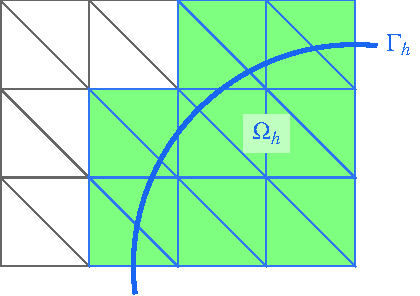
\includegraphics[width=0.4\linewidth]{dominioficticio.pdf}
	\hfil
	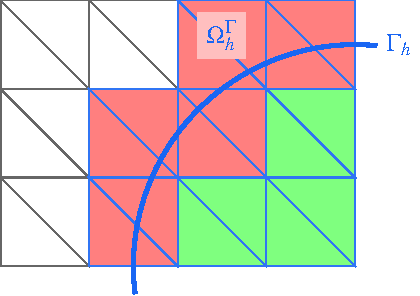
\includegraphics[width=0.4\linewidth]{dominiofrontera.pdf}
	\caption{Izquierda: Dominio ficticio $\Omega_h$ compuesto por los triángulos que interceptan $\Omega$. Derecha: Dominio frontera $\Omega_h^\Gamma$ compuesto por los triángulos que interceptan $\Gamma_h$ 		\label{fig:dominioficticio}}
	
\end{figure}

A continuación planteamos extender la solución de la ecuación \ref{eqn:edpmodelo} a una función $u$ definida sobre $\Omega_h$, y que es solución del siguiente problema:
\begin{align}
	-\Delta u+\beta u  = f &\text{ en }  \Omega_h\\
	u = g& \text{ en } \Gamma_h
\end{align}
donde $\beta\geq 0$, y suponemos que $g$ está definida en $\Omega^\Gamma_h$, de manera que las condiciones de borde toman la forma 
\begin{align}
	u = g + \phi_h p\text{, en } \Omega^\Gamma_h
\end{align}
%por medio de la siguiente formulación variacional: Encontrar $u$  en  $\Omega_h$, y $p$  en $  \Omega_h^\Gamma$ tales que
%\begin{equation}
%\begin{split}
%	\int_{\Omega_h}\nabla u \cdot \nabla v +\int_{\Omega_h}\beta uv - \int_{\partial \Omega_h}v(\nabla u \cdot n )
%	+ \gamma  \int_{\Omega_h^\Gamma} (u-\phi_h p) (v-\phi_h q) &
%	\\
%	\qquad\qquad\qquad\qquad\qquad\qquad=\int_{\Omega_h} fv + \gamma \int_{\Omega_h^\Gamma} g (v-\phi_h q)&,\forall v \text{ en } 
%	\Omega_h,q  \text{ en }  \Omega_h^\Gamma 
%\end{split}
%\end{equation}
%donde $\gamma>0$. 
%
%Para resolver el problema de manera adecuada es necesario incluir términos de estabilización que aseguren la existencia de solución en el dominio ficticio.
Definimos los espacios de elementos finitos sobre $\Omega_h$ y $\Omega_h^\Gamma$ respectivamente
\begin{align}
	V_h^{(k)}&= \left\{ v \in H^1(\Omega_h):\left.v\right\vert_T \in \mathbb{P}_k(T),\forall T \in \mathcal{T}_h\right\}\\
	Q_h^{(k)}&= \left\{ q \in H^1(\Omega_h^\Gamma):\left.q\right\vert_T \in \mathbb{P}_k(T),\forall T \in \mathcal{T}_h^\Gamma\right\}\\
	W_h^{(k)}&=	V_h^{(k)}	\times 	Q_h^{(k)}
\end{align}

La discretización de la solución de la  ecuación  \ref{eqn:edpmodelo} en el dominio ficticio, $u_h$ y la aproximación de la frontera libre, $\phi_h$ pueden utilizar polinomios de diferente grado ($k$ y $l$ respectivamente).

\subsection{Problema variacional discreto}
Definimos los siguientes términos de estabilización
\begin{equation}
	G_h(u,v)= \sigma h \sum_{E\in \mathcal{F}_h^\Gamma} \int_E \left[ \frac{\partial u}{\partial n} \right]
	\left[ \frac{\partial v}{\partial n} \right]	
\end{equation}
\begin{equation}
	J_h^{lhs}(u,v)=\sigma h^2 \sum_{T\in \mathcal{T}_h^\Gamma} \int_T (\Delta u-\beta u) (\Delta  v-\beta v),\quad
	J_h^{rhs}(v)=-\sigma h^2 \sum_{T\in \mathcal{T}_h^\Gamma} \int_T f(\Delta  v-\beta v),\quad 
\end{equation}
Donde $\mathcal{F}_h^\Gamma$ es el conjunto de aristas interiores de la malla $\mathcal{T}_h$ que pertenecen a elementos que interceptan a $\Gamma_h$
\[
\mathcal{F}_h^\Gamma  = \left\{ e : e\cap \partial\Omega^\Gamma_h =\emptyset,  \exists T\in \mathcal{T}_h: T\cap \Gamma_h \neq \emptyset \wedge e\in \partial T \right\}
\]
$G_h$ es el término de penalidad fantasma, \textit{ghost penalty} \citep{burman2010ghost}, y tiene por objetivo penalizar los saltos del gradiente en las aristas de la malla frontera. $J_h^{lhs}$ ayuda a estabilizar las oscilaciones de la solución aproximada en los elementos que cortan $\Gamma_h$ y es consistente: si $u$ es la solución exacta entonces $J_h^{lhs}(u,v)=J_h^{rhs}(v)$.

El problema discreto queda definido como sigue: 

Encontrar $(u_h,p_h)\in W_h^{(k)}$ tal que
\begin{equation}
	a_h(u_h,p_h;v_h,q_h)=l_h(v_h,q_h)\text{ para todo } (v_h,q_h)\in W_h^{(k)}
	\label{eqn:phifemdual}
\end{equation}
donde
\begin{equation}
	\begin{aligned}	
		a_h(w,p;v,q)&:=	\int_{\Omega_h}\nabla w \cdot \nabla v
		+	\int_{\Omega_h}\beta w  v
		- \int_{\partial \Omega_h} \frac{\partial w}{\partial n}  v
		+ \frac{\gamma}{h^2}  \int_{\Omega_h^\Gamma} (w-\frac{1}{h}\phi_h p) (v-\frac{1}{h}\phi_h q)
		\\
		&\qquad\qquad +G_h(w,v)+J_h^{lhs}(w,v)\\ 
		l_h(v,q)&:= \int_{\Omega_h} fv + \frac{\gamma}{h^2}  \int_{\Omega_h^\Gamma} g_h (v-\frac{1}{h}\phi_h q)+J_h^{rhs}(v)
	\end{aligned}
\end{equation}
donde $\gamma>0$ y $\sigma>0$ se escogen de manera independiente de $h$.

Si consideramos las formas bilineales
\begin{align}
	a_{11}(w,v)=&	\int_{\Omega_h}\nabla w \cdot \nabla v +	\int_{\Omega_h} \beta wv-\int_{\partial \Omega_h}\frac{\partial w}{\partial n}v+  \frac{\gamma}{h^2} \int_{\Omega_h^\Gamma}wv    
	+ G_h(w,v) + J_h^{lhs}(w,v)  %\nonumber
	\\
	a_{12}(p,v)=&	-\frac{\gamma}{h^3}  \int_{\Omega_h^\Gamma}  p \phi_h v
	\\
	a_{21}(w,q)=&	-\frac{\gamma}{h^3}  \int_{\Omega_h^\Gamma} w \phi_h q
	\\
	a_{22}(p,q)=&	\frac{\gamma}{h^4}  \int_{\Omega_h^\Gamma} \phi_h^2 p q
\end{align}

y las formas lineales
\begin{align}
	l_1(v) =&  \int_{\Omega_h} fv + \frac{\gamma}{h^2}  \int_{\Omega_h^\Gamma} g_h v +J_h^{rhs}(v)
	\\
	l_2(q)	=& - \frac{\gamma}{h^3}  \int_{\Omega_h^\Gamma} g_h \phi_h q
\end{align}
entonces
\[
\begin{aligned}
	a_h(w,p;v,q) &= a_{11}(w,v) + a_{12}(p,v)  + a_{21}(w,q)+ a_{22}(p,q) \\
	l(v,q) &=l_1(v)+l_2(q)
\end{aligned}
\]

de modo que el problema discreto se puede escribir como la siguiente ecuación
\[
\begin{matrix}
	&a_{11}(u,v) &+ &a_{12}(p,v) &  & \\
	+&a_{21}(u,q) &+ &a_{22}(p,q) & = & l_1(v)+l_2(q), \forall (v_h,q_h)\in W_h
\end{matrix}
\]
lo que nos lleva a un sistema matricial por bloques
\[
\begin{bmatrix}
	A_{11} & A_{12} \\
	A_{21} & A_{22} 
\end{bmatrix}
\begin{bmatrix}
	\bm{u} \\
	\bm{p} 
\end{bmatrix}=
\begin{bmatrix}
	\bm{l}_1 \\
	\bm{l}_2
\end{bmatrix}
\]
donde observamos que $(A_{12})^T = A_{21}$, pues \[
[A_{12}]_{ij}=a_{12}(w_j,v_i)=	-\frac{\gamma}{h^3}  \int_{\Omega_h^\Gamma} \phi_h w_j v_i=
a_{21}(v_i,w_j)=[A_{21}]_{ji}
\]
Asi los problemas variacionales para aproximar la presión intracelular, $p_h$ y la concentración de nutrientes $c_h$ pueden escribirse  partir de la ecuación  
\ref{eqn:phifemdual}:

Para $\beta=1$, $g=0$, encontrar $(c_h,w_h)\in W_h^{(k)}$ tal que
\begin{equation}
	a_h(c_h,w_h;v_h,w_h)=l_h(v_h,q_h)\text{ para todo } (v_h,q_h)\in W_h^{(k)}
	\label{eqn:problemach}
\end{equation}

Para $\beta=0$, $g=\kappa_h$, encontrar $(p_h,w_h)\in W_h^{(k)}$ tal que
\begin{equation}
	a_h(p_h,w_h;v_h,w_h)=l_h(v_h,q_h)\text{ para todo } (v_h,q_h)\in W_h^{(k)}
	\label{eqn:problemaph}
\end{equation}
donde $\kappa_h:\Omega^\Gamma \to\mathbb{R}$ es una aproximación de la curvatura de $\Gamma$.
\subsection{Existencia y unicidad de solución para el problema discreto}
En los resultados expuestos a continuación $\|\cdot\|_{k,D}$ denota la norma de $H^k(D)$ y $|\cdot|_{k,D}$ la respectiva seminorma. Además según  \citep{lozinski2019cutfem,duprez2020phi,duprez2022varphi} se establecen las siguientes premisas para el análisis teórico del método propuesto para resolver la ecuación \ref{eqn:phifemdual}.
\begin{premisa}
	Existe un dominio $\Omega^\Gamma$, vecindad de $\Gamma$   que puede ser cubierto por conjuntos abiertos $\mathcal{O}_i$, $i=1,\ldots,I$ y se puede introducir en cada $\mathcal{O}_i$ coordenadas locales $\xi_1$,\ldots, $\xi_d$ con $\xi_d=\phi$ tales que $\frac{\partial \xi}{\partial x^\alpha}$ y $\frac{\partial x}{\partial \xi^\alpha}$ hasta el orden $k+1$ están acotadas por algún $C_0>0$. Además $|\nabla \phi|\geq m$ en $\Omega_h^\Gamma$ para algún $m>0$
\end{premisa}
\begin{premisa}
	$\Omega_h^\Gamma\subset \Omega^\Gamma$ y $|\nabla \phi_h|\geq \frac{m}{2}$ en $\Omega_h^\Gamma$.
\end{premisa}
\begin{premisa}
	La frontera aproximada $\Gamma_h$ puede ser cubierta por subregiones $\left\{ \Pi_k\right\}_{k=1,,N_\Pi} $ con las siguientes propiedades:
	\begin{itemize}
		\item Cada $\Pi_k$ esta compuesta de un elemento $T_k$ contenido en  $\Omega$ y algunos elementos interceptados por $\Gamma$, es decir $\Pi_k = T_k \cup \Pi_k^\Gamma$ donde $T_k\in\mathcal{T}_h \subset \overline{\Omega}$, $\Pi_k^\Gamma\subset \mathcal{T}^\Gamma_h$ y $ \Pi_k^\Gamma$ contiene a lo mas $M$ elementos.
		\item Cada elemento en una subregión $\Pi_k$ comparte al menos un lado con otro elemento de la misma subregión. En particular, $T_k$ comparte un lado $F_k$ con un elemento en $\Pi_k^\Gamma$
		\item $\mathcal{T}^\Gamma_h = \cup_{k=1}^{N_\Pi} \Pi_k^\Gamma$ y $\Gamma_h^i = \cup_{k=1}^{N_\Pi} F_k$
		\item $\Pi_k$ y $\Pi_l$ son disjuntos si $k\neq l$.
	\end{itemize}
\end{premisa}
\begin{figure}[H]	
	\centering\hfil
	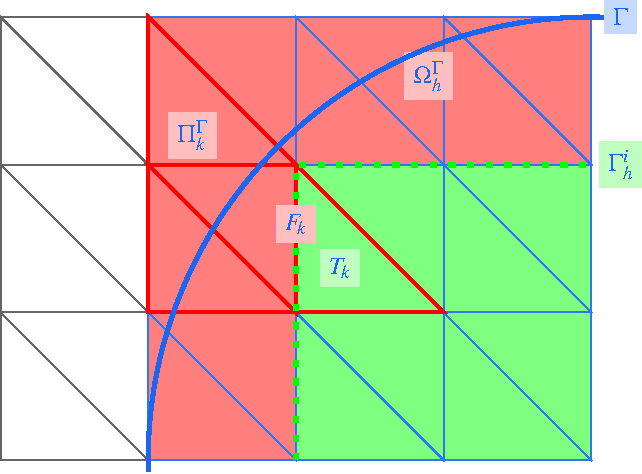
\includegraphics[width=0.4\linewidth]{subregionfrontera.pdf}
	\hfil
	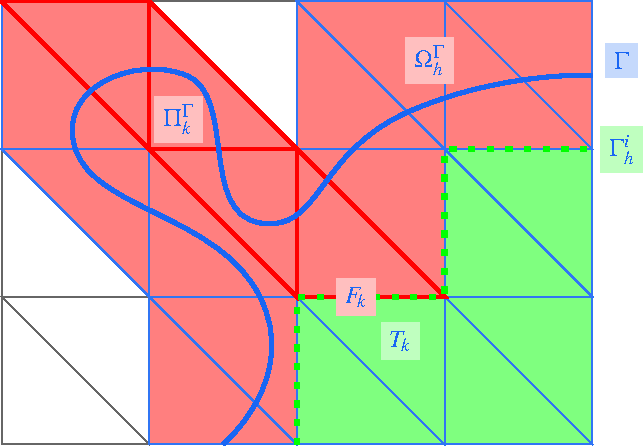
\includegraphics[width=0.4\linewidth]{subregionfronteranocontigua.pdf}
	\caption{Izquierda: Subregión $\Pi_k$, en borde rojo, compuesta de un elemento $T_k$ en $\overline{\Omega}$ y elementos $\Pi_k^\Gamma$ que interceptan $\Gamma$, la arista $F_k$ forma parte de  $\Gamma_h^i$ la frontera de $\Omega_h\setminus\Omega_h^\Gamma$ que se muestra con lineas verdes segmentadas. Derecha: Se muestran elementos frontera que no satisfacen la Premisa 2, esto indica que la malla no está suficientemente refinada. }
	\label{fig:dominiofrontera}
\end{figure}
La última premisa asegura que un elemento del dominio frontera este siempre contiguo a un elemento contenido en el dominio físico y descarta el caso mostrado en la Figura \ref{fig:dominiofrontera} donde la frontera esta ondulada y por lo tanto el ancho de subregión $\Pi_k$ es mayor que $h$. 


Recordemos el lema visto en \cite[Lema 3.2 en p.~1013]{duprez2020phi}:
\begin{lema}\label{lema:triangulo}
	Sea $T$ un triangulo, $E$ uno de sus lados y $p$ un polinomio en $T$ de grado $s$, tal que $p=\frac{\partial p}{\partial n}=0$ en E y $\Delta p=0$ en $T$. Entonces $p=0$ en $T$.
\end{lema}
A continuación adaptamos un resultado de
\cite[Lema 3.5 en p.~82]{lozinski2019cutfem}
\begin{lema}\label{lema:alfa}
	Sea $B_h$ la región entre $\Gamma_h$ y $\partial\Omega_h$. Para todo $\beta,\lambda>0$, existe $\alpha<1$ tal que para todo $v\in V_h^{(k)}$
	\[
	\int_{B_h} |\nabla v|^2 \leq \alpha |v|^2_{1,\Omega_h}+ \lambda h \sum_{E\in \mathcal{F}_h^\Gamma}\left\| \left[ \frac{\partial v}{\partial n}\right] \right\|^2_{0,E}+\lambda h^2 \sum_{T\in \mathcal{T}_h^\Gamma} \|\Delta v-\beta v\|^2_{0,T}+ \lambda \beta^2 h^2\|v\|^2_{0,\Omega^\Gamma_h}
	\]
\end{lema}	
\begin{proof}[Prueba]
	Dado $\lambda>0$, consideramos una descomposición de $\Omega_h^\Gamma$ en elementos $\{\Pi_k\}$ y definimos
	\[
	F(\Pi_k,v)=\dfrac{|v|^2_{1,\Pi_k^\Gamma} -  \lambda h \displaystyle\sum_{E\in \mathcal{F}_k}\left\| \left[ \dfrac{\partial v}{\partial n}\right] \right\|^2_{0,E}-\lambda h^2 \displaystyle\sum_{T\subset \Pi_k} \|\Delta v\|^2_{0,T}}{ |v|^2_{1,\Pi_k}}
	\]
	y \[
	\alpha = \max_{\Pi_k,v\neq 0} F(\Pi_k,v)
	\]
	donde el subconjunto $\mathcal{F}_k \subset \mathcal{F}_h^\Gamma$ esta compuesto por los lados internos en $\Pi_k$.
	
	Como  $|v|_{1,\Pi_k^\Gamma}\leq  |v|^2_{1,\Pi_k}$ entonces $\alpha \leq 1$. Supongamos que $\alpha=1$ entonces existen $\Pi_k$, $v$ tales que
	\[
	|v|^2_{1,\Pi_k}=	|v|^2_{1,\Pi_k^\Gamma} -  \lambda h \sum_{E\in \mathcal{F}_k}\left\| \left[ \frac{\partial v}{\partial n}\right] \right\|^2_{0,E}-\lambda h^2 \sum_{T \subset\Pi_k } \|\Delta v\|^2_{0,T} 
	\]
	y por lo tanto
	\[
	|v|^2_{1,T_k}+  \lambda h \sum_{E\in \mathcal{F}_k}\left\| \left[ \frac{\partial v}{\partial n}\right] \right\|^2_{0,E}+\lambda h^2 \sum_{T  \subset\Pi_k} \|\Delta v\|^2_{0,T} =0
	\]
	Como $|v|^2_{1,T_k}=0$ entonces existe $c\in\mathbb{R}$, tal que $v_h=c$ en $T_k$. Aplicamos el Lema \ref{lema:triangulo} a $v-c$ de donde $v_h=c$ en $\Pi_k$ y por lo tanto 	$|v|^2_{1,\Pi_k}=0$. Asi $\alpha<1$	y
	\[
	|v|^2_{1,\Pi_k^\Gamma}\leq \alpha	|v|^2_{1,\Pi_k} +  \beta h \sum_{E\in \mathcal{F}_k}\left\| \left[ \frac{\partial v}{\partial n}\right] \right\|^2_{0,E} + \beta h^2 \sum_{T \subset\Pi_k } \|\Delta v\|^2_{0,T} 
	\]
	sumando respecto de las subregiones $\Pi_k$ y como $B_h\subset \Omega_h^\Gamma$ entonces
	\[
	\int_{B_h} |\nabla v|^2 \leq \alpha |v|^2_{1,\Omega_h}+ \beta h \sum_{E\in \mathcal{F}_h^\Gamma}\left\| \left[ \frac{\partial v}{\partial n}\right] \right\|^2_{0,E}+\beta h^2 \sum_{T\in \mathcal{T}_h^\Gamma} \|\Delta v\|^2_{0,T}
	\]
	por ultimo aplicamos la desigualdad triangular en cada elemento $T$, $\|\Delta v\|^2_{0,T}\leq \|\Delta v-\beta v\|^2_{0,T}+\|\beta v\|^2_{0,T}$.
\end{proof}	
Consideremos las siguientes desigualdades adaptadas de 
\cite[Lema 3.1 y Lema 3.4]{lozinski2019cutfem}
%\begin{lema}[\protect{\citep[Lema 3.1]{lozinski2019cutfem}}]
\begin{lema}
	\label{lema:trazaraiz}
	Para toda función $v\in H^1(\Omega_h^\Gamma)$ 
	\[
	\|v\|^2_{0,\Omega^\Gamma_h}
	\leq C \left( h\|v\|^2_{0,\Gamma_h} + h^2 |v|^2_{1,\Omega^\Gamma_h}\right)
	\]
\end{lema}
%\begin{lema}[\protect{\cite[Lema 3.4]{lozinski2019cutfem}}]
\begin{lema}
	\label{lema:traza}
	Para toda función $v\in H^1(\Omega_h^\Gamma)$ 
	\[
	\sum_{E\in\mathcal{F}_h^\Gamma} \|v\|^2_{0,E} \leq C \left( \frac{1}{h}\|v\|^2_{0,\Omega_h^\Gamma} + h |v|^2_{1,\Omega^\Gamma_h}\right)
	\]  y
	\[
	\|v\|^2_{0,\partial\Omega_h} \leq C \left( \|v\|^2_{0,\Gamma_h} + h\|v\|^2_{1,\Omega^\Gamma_h}\right)
	\]
\end{lema}
Según el siguiente lema visto en 
\cite[Lema 3.5]{duprez2022varphi}, \cite[Lema 1.46]{di2011mathematical}.
\begin{lema}[Desigualdad de la traza discreta]\label{lema:trazaq}
	Para toda función $v_h$ polinomial a trozos en $\mathcal{T}_h^\Gamma$, \[\|v_h\|_{0,\Gamma_h} \leq \frac{C}{\sqrt{h}} \|v_h\|_{0,\Omega^\Gamma_h}\]
	con constante $C>0$ dependiendo del máximo grado de los polinomios en $v_h$ y de las constantes dadas en las Premisas 1-2.
\end{lema}	

%\begin{lema}[Desigualdad de la traza discreta \cite[Lema 1.46]{di2011mathematical}] 
%c
%\end{lema}	
%\begin{lema}
%	Sea $B_h$ la región entre $\Gamma_h$ y $\partial\Omega_h$, 
%	$B_h=\{\phi>0\}\cap\Omega_h$
%\end{lema}
\begin{prop} Si $\gamma$ y $\sigma$ son suficientemente grandes, existe $M>0$ tal que
	\[
	\begin{aligned}
		a_h(v,q;v,q) \geq M \left(|v|^2_{1,\Omega_h}		
		+ 	 \frac{1}{h^2}\|v-\frac{1}{h}\phi_h q\|^2_{0,\Omega^\Gamma_h} +
		h \sum_{E\in \mathcal{F}_h^\Gamma} \left\| \left[ \frac{\partial v}{\partial n} \right]\right \|^2_{0,E}+
		h^2 \sum_{T\in \mathcal{T}_h^\Gamma}  \|\Delta  v\|^2_{0,T}
		\right)
	\end{aligned}
	\]
\end{prop}
\begin{proof}[Prueba]
	Sea $v_h\in V_h^{(k)}$ y $B_h =\{\phi_h>0\}\cap\Omega_h$ con $\partial B_h=\partial\Omega_h \cup \Gamma_h$. Entonces procedemos a expresar la integral de linea sobre la frontera del dominio ficticio como una  integral sobre $B_h$ y los saltos del gradiente en las aristas de los elementos del dominio frontera, como se ilustra a continuación:
	
	%\[
	%\begin{aligned}
	%	\int_{\partial \Omega_h} (\nabla u\cdot n) v
	%	&=\int_{\partial \Omega_h} (\nabla u\cdot n) v-
	%	\int_{\Gamma_h} \frac{1}{|\nabla \phi|}(\nabla u\cdot n) v 
	%	+\int_{\Gamma_h} \frac{1}{|\nabla \phi|}(\nabla u\cdot n - \frac{1}{h}q\phi) v \\
	%	&=\int_{B_h} (v \Delta u + \nabla u\cdot \nabla v) 
	%	+\int_{\Gamma_h} \frac{1}{|\nabla \phi|}(\nabla u\cdot \nabla \phi - \frac{1}{h}q\phi) v 
	%\end{aligned}
	%\]
	\begin{figure}[H]
		%	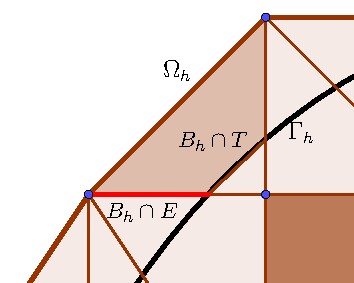
\includegraphics[valign = c, width = .3\linewidth]{bilinealbh.pdf}
		\centering
		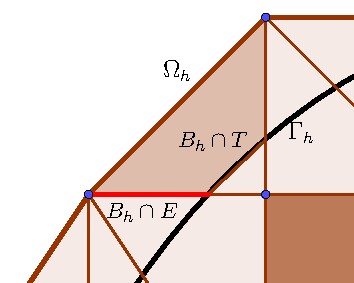
\includegraphics[width = .4\linewidth]{bilinealbh.pdf}
		\caption{Descomposición de la integral de linea sobre $\partial \Omega_h$ en función de las aristas de los elementos del dominio frontera.}
	\end{figure}
	\[
	\begin{aligned}
		\int_{\partial \Omega_h} \frac{\partial u}{\partial n} v
		&=\int_{\partial B_h} \frac{\partial u}{\partial n} v+
		\int_{\Gamma_h} \frac{\partial u}{\partial n} v \\
		&= \sum_{T\in \mathcal{T}_h^\Gamma} \int_{\partial (B_h \cap T)} \frac{\partial u}{\partial n} v - \sum_{E\in \mathcal{F}_h^\Gamma}\int_{B_h \cap E} \left[\frac{\partial u}{\partial n} 
		\right]v+	\int_{\Gamma_h} \frac{\partial u}{\partial n} v \\
		&=\int_{B_h} (v \Delta u + \nabla u\cdot \nabla v) 
		- \sum_{E\in \mathcal{F}_h^\Gamma}\int_{B_h \cap E} \left[\frac{\partial u}{\partial n} 
		\right]v+
		\int_{\Gamma_h} \frac{\partial u}{\partial n} v 
	\end{aligned}
	\]
	%\[
	%\begin{aligned}
	%	\int_{\partial \Omega_h} (\nabla u\cdot n) v
	%	&=\int_{\Omega_h} (v \Delta u + \nabla u\cdot \nabla v) \\
	%	& =\int_{\Omega^\Gamma_h} (v \Delta u + \nabla u\cdot \nabla v)+\int_{\Omega^i_h} (v \Delta u + \nabla u\cdot \nabla v) 
	%\end{aligned}
	%\]
	luego
	\[
	\begin{aligned}	
		a_h(u,p;v,q)&=\int_{\Omega_h} \nabla u\cdot \nabla v +\int_{\Omega_h} \beta uv - 
		\int_{B_h} (v \Delta u + \nabla u\cdot \nabla v) 
		-\int_{\Gamma_h} \frac{\partial u}{\partial n} v 
		\\
		&+ \sum_{E\in \mathcal{F}_h^\Gamma}\int_{B_h \cap E} \left[\frac{\partial u}{\partial n} 
		\right]v + \frac{\gamma}{h^2}\int_{\Omega^\Gamma_h} (u-\frac{1}{h}\phi p)(v-\frac{1}{h}\phi q) +G_h(u,v)+J_h^{lhs}(u,v)
	\end{aligned}
	\]
	y
	\[
	\begin{aligned}	
		a_h(v,q;v,q)&=\int_{\Omega_h} |\nabla v |^2 +\int_{\Omega_h} \beta |v |^2 - 
		\int_{B_h} v \Delta v -\int_{B_h} |\nabla v|^2
		-	\int_{\Gamma_h} v\frac{\partial v}{\partial n}  
		\\
		&+ \sum_{E\in \mathcal{F}_h^\Gamma}\int_{B_h \cap E} \left[\frac{\partial v}{\partial n} 
		\right]v+ \frac{\gamma}{h^2}\int_{\Omega^\Gamma_h} (v-\frac{1}{h}\phi q)^2	+G_h(v,v)+J_h^{lhs}(v,v)
	\end{aligned}
	\]
	por el Lema \ref{lema:trazaq}
	\[
	\begin{aligned}
		-\int_{\Gamma_h} v\frac{\partial v}{\partial n} & \geq - \|v\|_{0,\Gamma_h}\|\nabla v \cdot n\|_{0,\Gamma_h}
		\geq - \frac{C^2}{h}\|v-\frac{1}{h}\phi q\|_{0,\Omega^\Gamma_h}\|\nabla v \|_{0,\Omega^\Gamma_h}\\
		& \geq -\frac{1}{2}\left(
		\frac{C^3}{\epsilon h^2}\|v-\frac{1}{h}\phi q\|^2_{0,\Omega^\Gamma_h} + \epsilon C | v |^2_{1,\Omega^\Gamma_h}
		\right)
	\end{aligned}
	\]
	%Del Lema \ref{lema:traza}:
	%\[
	%\begin{aligned}
	%\left|
	%\int_{\Gamma_h} \frac{1}{|\nabla \phi|}(\nabla v\cdot \nabla \phi - \frac{1}{h}q\phi) v \right|
	%&\leq \frac{C}{h} \|\nabla v\cdot \nabla \phi - \frac{1}{h}q\phi \|_{0,\Omega_h^\Gamma}\| v\|_{0,\Omega_h^\Gamma} \\
	%&\leq \frac{1}{2} \left( \frac{  C^2}{\epsilon h^2}\|\nabla v\cdot \nabla \phi - \frac{1}{h}q\phi \|^2_{0,\Omega_h^\Gamma} +\epsilon\| v\|^2_{0,\Omega_h^\Gamma}\right)\quad \text{(Desigualdad de Young)}
	%\end{aligned}
	%\]
	\[
	\sum_{E\in \mathcal{F}_h^\Gamma}\int_{B_h \cap E} \left[\frac{\partial v}{\partial n} 
	\right]v \geq 
	-\frac{1}{2} \left( \frac{\epsilon}{h} \sum_{E\in \mathcal{F}_h^\Gamma} \|v\|^2_{0,E} + \frac{h}{\epsilon }
	\sum_{E\in \mathcal{F}_h^\Gamma}\left \| \left[\frac{\partial v}{\partial n} 
	\right] \right \|^2_{0,E} 
	\right)\quad \text{(Desigualdad de Young)}
	\]
	del Lema \ref{lema:traza}:
	\[
	-\frac{\epsilon}{h}\sum_{E\in\mathcal{F}_h^\Gamma} \|v\|^2_{0,E} \geq -\frac{\epsilon C}{h} \left( \frac{1}{h}\|v\|^2_{0,\Omega_h^\Gamma} + h |v|^2_{1,\Omega^\Gamma_h}\right)
	\] 
	Como $B_h\subset \Omega_h^\Gamma$
	\[
	\begin{aligned}
	\left|	\int_{B_h} \beta v^2 -	\int_{B_h} v \Delta v
	\right|\leq  \|  v \|_{0,\Omega_h^\Gamma}
	\|\Delta v -\beta v\|_{0,\Omega_h^\Gamma}\leq 
	\frac{1}{2} \left( \frac{\epsilon C}{h^2}  \|  v \|^2_{0,\Omega_h^\Gamma} + \frac{h^2}{\epsilon C }
	\|\Delta v -\beta v \|^2_{0,\Omega_h^\Gamma}
	\right)\\
	\text{(Desigualdad de Young)}			
	\end{aligned}
	\]
	del Lema \ref{lema:alfa}
	\[
	\int_{B_h} |\nabla v|^2 \leq \alpha |v|^2_{1,\Omega_h}+ \lambda h \sum_{E\in \mathcal{F}_h^\Gamma}\left\| \left[ \frac{\partial v}{\partial n}\right] \right\|^2_{0,E}+\lambda h^2 \sum_{T\in \mathcal{T}_h^\Gamma} \|\Delta v-\beta v\|^2_{0,T}+ \lambda \beta^2 h^2\|v\|^2_{0,\Omega^\Gamma_h}
	\]
	
	por el Lema \ref{lema:trazaq} y como $v=v-\frac{1}{h}\phi q$ en $\Gamma_h$
	\[
	-\|v_h\|^2_{0,\Gamma_h} \geq - \frac{C^2}{h} \|v_h-\frac{1}{h}\phi q\|_{0,\Omega^\Gamma_h}\]
	luego
	\[
	\begin{aligned}	
		a_h(v,q;v,q)&\geq \int_{\Omega_h} |\nabla v |^2 + \int_{\Omega^i_h} \beta|v|^2 -
		\frac{1}{2} \left(\frac{ \epsilon C }{h^2} \|  v \|^2_{0,\Omega_h^\Gamma} + \frac{h^2}{\epsilon C}
		\|\Delta v-\beta v \|^2_{0,\Omega_h^\Gamma}
		\right)	\\	
		&-\alpha |v|^2_{1,\Omega_h} - \lambda h \sum_{E\in \mathcal{F}_h^\Gamma}\left\| \left[ \frac{\partial v}{\partial n}\right] \right\|^2_{0,E} -\lambda h^2 \sum_{T\in \mathcal{T}_h^\Gamma} \|\Delta v-\beta v\|^2_{0,T} - \lambda\beta^2 h^2 \|v\|^2_{0,\Omega_h^\Gamma}\\
		&
		-\frac{1}{2} \left( \frac{\epsilon}{h} \sum_{E\in \mathcal{F}_h^\Gamma} \|v\|^2_{0,E} + \frac{h}{\epsilon }
		\sum_{E\in \mathcal{F}_h^\Gamma}\left \| \left[\frac{\partial v}{\partial n} 
		\right] \right \|^2_{0,E} 
		\right)
		+ \frac{\gamma}{h^2}\int_{\Omega^\Gamma_h} (v-\frac{1}{h}\phi q)^2
		\\
		&	+		 \sigma h \sum_{E\in \mathcal{F}_h^\Gamma} \left\| \left[ \frac{\partial v}{\partial n} \right]\right \|^2_{0,E}+
		\sigma h^2 \sum_{T\in \mathcal{T}_h^\Gamma}  \|\Delta  v-\beta v\|^2_{0,T} -\frac{1}{2}\left(
		\frac{C^3}{\epsilon h^2}\|v-\frac{1}{h}\phi q\|^2_{0,\Omega^\Gamma_h} + \epsilon C| v |^2_{1,\Omega^\Gamma_h}
		\right)\\
		& \geq (1-\alpha- \epsilon C ) |v|^2_{1,\Omega_h}
		- \frac{\epsilon C}{h^2}   \|v\|^2_{0,\Omega_h^\Gamma}
		+ 	 \frac{\gamma-\frac{C^3}{2\epsilon }      }{h^2}\|v-\frac{1}{h}\phi q\|^2_{0,\Omega^\Gamma_h} \\
		& +		 (\sigma-\lambda-\frac{1}{2\epsilon}) h \sum_{E\in \mathcal{F}_h^\Gamma} \left\| \left[ \frac{\partial v}{\partial n} \right]\right \|^2_{0,E}+
		h^2(\sigma-\lambda-\frac{1}{2\epsilon C})  \sum_{T\in \mathcal{T}_h^\Gamma}  \|\Delta  v-\beta v\|^2_{0,T} \\
		& \geq (1-\alpha- 2\epsilon C ) |v|^2_{1,\Omega_h}		
		+ 	 \frac{\gamma- C^3 (\epsilon +\frac{1}{2\epsilon} ) }{h^2}\|v-\frac{1}{h}\phi q\|^2_{0,\Omega^\Gamma_h} \\
		& +		 (\sigma-\lambda-\frac{1}{2\epsilon}) h \sum_{E\in \mathcal{F}_h^\Gamma} \left\| \left[ \frac{\partial v}{\partial n} \right]\right \|^2_{0,E}+
		h^2(\sigma-\lambda-\frac{1}{2\epsilon C})  \sum_{T\in \mathcal{T}_h^\Gamma}  \|\Delta  v-\beta v\|^2_{0,T} 
	\end{aligned}
	\]
	donde $0<h\leq h_0:={\rm diam}(\Omega)$
	
	Si elegimos $0<\epsilon<\frac{1-\alpha}{2C}$, $\gamma> C^3 (\epsilon +\frac{1}{2\epsilon} )$, $\sigma_D > \max\left\{\lambda +\frac{1}{2\epsilon},
	\lambda +\frac{1}{2\epsilon C}\right\}$ entonces encontramos $M>0$ como
	\[
	M=\min\left\{1-\alpha-2\epsilon C,
	\gamma - C^3 (\epsilon +\frac{1}{2\epsilon} ),\sigma_D-\beta-\frac{1}{2\epsilon},\sigma_D-\beta-\frac{1}{2\epsilon C}
	\right\}\]
\end{proof}
\begin{teo}
	Las ecuaciones \ref{eqn:problemach},  para la concentración de nutrientes $c_h$,  y \ref{eqn:problemaph} para la presión intracelular $p_h$  tienen solución única. 
\end{teo}
\begin{proof}[Prueba]
	Si definimos \[\vertiii{v,q}_h=\left(|v|^2_{1,\Omega_h}				+ 	 \dfrac{1}{h^2}\|v-\dfrac{1}{h}\phi_h q\|^2_{0,\Omega^\Gamma_h} +
	h \sum_{E\in \mathcal{F}_h^\Gamma} \left\| \left[ \dfrac{\partial v}{\partial n} \right]\right \|^2_{0,E}+
	h^2 \sum_{T\in \mathcal{T}_h^\Gamma}  \|\Delta  v\|^2_{0,T}
	\right)\] entonces $\vertiii{\cdot}$ es una norma para $W_h^{(k)}$, pues si $\vertiii{v,q}_h=0$ entonces $v_x=v_y=0$ en $\Omega_h$ es decir $v$ es constante en todo $\Omega_h$ y como $v=\dfrac{1}{h}\phi_h$ entonces $v=0$ en $\Gamma_h$, y por lo tanto $v=0$ en $\Omega_h$. De igual modo $\|v-\dfrac{1}{h}\phi_h q\|^2_{0,\Omega^\Gamma_h}=0$ implica que $\phi_h q=0$ y al ser $q$ continua entonces $q=0$ en $\Omega^\Gamma_h$. Por lo tanto la única solución del problema homogéneo  $a_h(v,q;v,q)=0$ es la trivial, y al ser $W^{(k)}_h$ de dimensión finita el problema $a_h(v,q;v,q)=l_h(v_h,q_h)$  tendrá solución única.
\end{proof}

% Sea $T$ un triángulo y $E$ uno de sus lados, por el teorema de la traza $\|v\|^2_{0,E}\leq C\|v\|^2_{1,T}$
%Recordamos la desigualdad de la traza en \cite{riviere2005analysis} escalada: Existe una constante $C$ independiente de $h$ tal que
% \[
% \|v\|^2_{0,E}\leq C\left( \frac{1}{h}\|v\|^2_{0,T}+h| v|^2_{1,T}
% \right)
% \]
% luego 
%Recordemos el lema visto en \cite[Teorema 33.2 en p.~127]{duprez2020phi}: $\int_{\Gamma_h} |v|\leq $
%
%	\begin{tabular}{ccccc}
	%		$h$ & $\|u_h-u_{ex}\|_{L^2}$ & orden & $\|u_h-u_{ex}\|_{H^1}$ & order \\
	%		 \toprule 
	%		 
	%	\end{tabular}		


%Si suponemos que $f\in H^k(\Omega )$ entonces la solución de **** pertenece a $H^{k+2}(\Omega)$ y puede ser extendida por una función $u^*$ en  $H^{k+2}(\Omega)$ \cite[p. 268]{evans2010partial} y


\section{Extensión de la velocidad}
Para poder resolver la ecuación \ref{eqn:evolucionconjuntodenivel} de evolución de la frontera libre  es preciso encontrar una función $S=(S_1,S_2)$ que extienda la velocidad $V=(v_1,v_2)$ definida solo en la frontera del tumor $\Gamma_h$. El método \ref{eqn:phifemdual} aplicado a la presión y a la concentración de nutrientes permite obtener una aproximación de la velocidad de crecimiento del tumor en la región $\Omega_h^\Gamma$ y no solamente en la frontera $\Gamma_h$.

Si $A=\begin{bmatrix} \phi_x^2 &  \phi_{x}\phi_{y} \\ \phi_{x}\phi_{y} & \phi_y^2 \end{bmatrix}$, entonces $S_i$ es solución del problema elíptico:
\begin{equation}
	\begin{aligned}
		\nabla \cdot (A \nabla u)=0 & \text{ en }  \mathcal{O}\setminus \Gamma \\
		(A \nabla u) \cdot n=0 &	 \text{ en }  \partial \mathcal{O}\\
		u=v_i &	 \text{ en } \Gamma
	\end{aligned}
	\label{eqn:problemaextension}
\end{equation}
Sin embargo a menos que $A$ sea definida positiva no podemos asegurar unicidad de la solución y ya que deseamos obtener una extensión de la velocidad suficientemente suave en todo $\mathcal{O}$, por lo que es necesario incluir un término de viscosidad artificial para $\epsilon$ pequeño:
\begin{equation}
	\begin{aligned}
		\nabla \cdot ((A+\epsilon I) \nabla u)=0 & \text{ en }  \mathcal{O}\setminus \Gamma \\
		((A+\epsilon I) \nabla u) \cdot n=0 &	 \text{ en }  \partial \mathcal{O}\\
		u=v_i &	 \text{ en } \Gamma
	\end{aligned}
\end{equation}
Para encontrar $S_h=(S_{h,1},S_{h,2})$, una aproximación numérica de la extensión de la velocidad se define el siguiente espacio de elementos finitos sobre $\mathcal{O}$: 
\[
M_h= \left\{
v \in H^1(\mathcal{O}):\left.v\right\vert_T \in \mathbb{P}_k(T),\forall T \in \mathcal{T}^\mathcal{O}_h
\right\}
\]
de modo que el problema a resolver es el siguiente:

Encontrar $S_{h,i} \in M_{h},p_h\in Q^k_h$:
\begin{equation}
	\begin{aligned}
		\int_\mathcal{O} ((A+\epsilon I) \nabla S_{h,i})\cdot\nabla v_h +  \frac{\gamma}{h^2}  \int_{\Omega_h^\Gamma} (S_{h,i}-\frac{1}{h}\phi_h p_{h}) (v_{h}-\frac{1}{h}\phi_h q_{h})&=
		\frac{\gamma}{h^2}  \int_{\Omega_h^\Gamma} v_i(v_{h}-\frac{1}{h}\phi_h q_{h})\\
		&\forall v_{h} \in M_{h},q_h\in Q^k_h
	\end{aligned}
	\label{eqn:problemaSh}
\end{equation}
\begin{prop}
	El problema de extensión de la velocidad dado por la ecuación \ref{eqn:problemaSh} tiene solución única.	
	\label{prop:extension}
\end{prop}
\begin{proof}[Prueba]
	Como
	\[
	(x,y)^T(A+\epsilon I)(x,y)=(x\phi_x+y\phi_y)^2+\epsilon(x^2+y^2)
	\geqslant \epsilon(x^2+y^2)
	\]
	entonces para $v_i=0$ tenemos que
	\[
	0\leqslant 	\epsilon|v_h|^2_{1,\mathcal{O}} +  
	\frac{\gamma}{h^2} \|v_{h}-\frac{1}{h}\phi_h p_{h}\|^2_{0,\Omega_h^\Gamma}  
	\leqslant 	\int_\mathcal{O} ((A+\epsilon I) \nabla v_{h})\cdot\nabla v_h+
	\frac{\gamma}{h^2}  \int_{\Omega_h^\Gamma}  (v_{h}-\frac{1}{h}\phi_h p_{h})^2 =0
	\]
	por lo tanto $\partial_x v_h=0$ y $\partial_y v_h=0$, esto implica que $v_h=c$ es constante en $\mathcal{O}$ y como además $v_h=0$ en $\Gamma_h$  obtenemos que $v_h=0$ y $p_h=0$. Como la única solución del problema homogéneo asociado a la ecuación \ref{eqn:problemaSh} es la trivial y tanto $M_{h}$ como $Q^k_h$ son de dimensión finita podemos concluir la existencia y unicidad del problema de extensión de la velocidad.
\end{proof}
\comentario{
	\[
	\begin{aligned}
		-\Delta u =0&\text{ en }\Omega \\
		u=g_D &\text{ en }\Gamma \\
		\left[\frac{\partial u}{\partial n}\right] = 0&\text{ en }\Gamma\\
		\frac{\partial u}{\partial n} = g_N &\text{ en } \partial\Omega \\
	\end{aligned}
	\]
	\[
	\int_{\Omega_{h,1}} \nabla u \cdot \nabla u - \int_{\partial \Omega_{h,1}}v \nabla u\cdot n =0
	\]
	\[
	u_1 = g +p_1\phi ,\quad u_2 = g  +p_2\phi 
	\]
	\[
	y_1 + \nabla u_1=0,\quad y_2 + \nabla u_2=0
	\]
	\[
	y_1\nabla \phi -y_2\nabla \phi =0,\text{ en }\Omega_h^\Gamma
	\]
	\[
	Z_h = \left\{z:\Omega_h^\Gamma \to\mathbb{R}^2: z|_T \in \mathbb{P}^k(T) \times \mathbb{P}^k(T), \forall T \in \Omega_h^\Gamma  \right\}
	\]
	Encontrar $u_{h,i} \in V_{h,i},p_h\in Q^k_h, 	y_{h,i} \in Z_h$:
	\[
	\begin{aligned}
		\sum_{i=1}^{2}\int_{\Omega_{h,i}} \nabla u_{h,i} \cdot \nabla v_{h,i} &+ 	\sum_{i=1}^{2}\int_{\partial \Omega_{h,i}}v_{h,i} (y_{h,i}\cdot n )\\
		& +\frac{\gamma_p}{h^2} \sum_{i=1}^{2} \int_{\Omega_h^\Gamma} (u_{h,i}-\frac{1}{h}\phi_h p_{h,i}) (v_{h,i}-\frac{1}{h}\phi_h q_{h,i})
		\\
		& +\gamma_u \sum_{i=1}^{2}\int_{\Omega_h^\Gamma} 
		(y_{h,i} + \nabla u_{h,i})\cdot 
		(z_{h,i} + \nabla v_{h,i})
		\\
		& +\frac{\gamma_y}{h^2} \int_{\Omega_h^\Gamma} 
		(y_{h,1}\cdot \nabla \phi_{h}-
		y_{h,2}\cdot \nabla \phi_{h})(z_{h,1}\cdot \nabla \phi_{h}-
		z_{h,2}\cdot \nabla \phi_{h})
		\\
		& +  \sum_{i=1}^{2} \left( G_h(u_{h,i},v_{h,i})+ J_h^{lhs}(y_{h,i},z_{h,i}) \right)\\
		&	=\sum_{i=1}^{2} \int_{\Omega_{h,i}} fv_{h,i} + \frac{\gamma_p}{h^2}  \sum_{i=1}^{2} \int_{\Omega_h^\Gamma} g_h (v_{h,i}-\frac{1}{h}\phi_h q_{h,i})+\sum_{i=1}^{2}J_h^{rhs}(z_{h,i}),\\
		&\forall v_{h,i} \in V_{h,i},q_h\in Q^k_h, 	z_{h,i} \in Z_h
	\end{aligned}
	\]
	donde 
	\[
	J_h^{lhs}(y,z) = \gamma_{div} \int_{\Omega_h^\Gamma} (\nabla \cdot y)(\nabla \cdot z),\qquad
	J_h^{rhs}(z) = \gamma_{div} \int_{\Omega_h^\Gamma} (\nabla \cdot z)f
	\]
}
\comentario{
	\section{Evolución de la frontera libre}
	La ecuación que rige el crecimiento del tumor en la frontera libre es
	\[
	\frac{\partial \phi}{ \partial t} + V_n \|\nabla \phi(x(t),y(t))\|=0,\forall t>0
	\]
	donde $(x(t),y(t))\in \Gamma, \forall t>0$, y $V_n$ es la velocidad de crecimiento en la dirección normal a la frontera. 
	
	Escogiendo $a(x,y,t)$  tal que $a(x,y,t)=V_n n, \forall (x(t),y(t))\in \Gamma$ plantemos la siguiente ecuación de advección.
	
	\begin{equation}
		\label{eqn:phi}
		\frac{\partial \phi}{ \partial t} + a \cdot \nabla \phi =0
	\end{equation}
	podemos discretizar \eqref{eqn:phi} con el método de curvas características, $X(s,t_{n},x)$ tal que para $x$ y $t_{n+1}$ fijos, satisfacen la siguiente ecuación diferencial:
	\begin{equation}
		\frac{d}{ds}X(s,t_{n+1},x)=a(s,X(s,t_{n+1},x)),s\in]t_n,t_{n+1}[,
		X(t_{n+1},t_{n+1},x)=x.
		\label{eqn:caracteristicas}
	\end{equation}
	y por lo tanto
	\[
	0=\frac{d}{ds} \phi(s,X(s,t_{n+1},x))\approx
	\frac{\phi(t_{n+1},X(t_{n+1},t_{n+1},x))-\phi(t_{n},X(t_{n},t_{n+1},x)) }{t_{n+1}-t_{n}}
	\]
	luego
	\[
	\phi(t_{n+1},x)=\phi(t_{n},X(t_{n},t_{n+1},x))
	\]
	De la ecuación \ref{eqn:caracteristicas}  podemos expresar
	\[
	X(t_{n},t_{n+1},x)=x-
	\int_{t_{n}}^{t_{n+1}}	a(s,X(s,t_{n+1},x))\, ds
	\]
	por lo tanto si aplicamos una aproximación por integración numérica
	\[
	\phi(t_{n+1},x)=\phi(t_{n},x-\Delta t a(t_{n+1},x))
	\]
	\cite{gross2011numerical}
	\[
	X(t_{n},t_{n+1},x)=x-\Delta t a(t_n,x)
	\]
}
\section{Aproximación de la curvatura}

La normal a la frontera del tumor, $n_\Gamma$ está definida por medio de:
\[
n_\Gamma = \frac{\nabla \phi}{\|\nabla \phi \|}
\]
y puede ser aproximada en el espacio $X_h=\{v\in [C^0(\mathcal{O})]^2: v|_K\in [\mathbb{P}_1(K)]^2,\forall K\in \mathcal{T}_h\}$ resolviendo el siguiente problema: 

Encuentre $N_h\in \mathcal{X}_h$ tal que 
\begin{equation}
	\left( N_h ,v \right)_{\mathcal{O}}=
	\left( \frac{\nabla \phi}{\|\nabla \phi \|} ,v \right)_{\mathcal{O}},\forall v	\in \mathcal{X}_h
\end{equation}

Es necesario además encontrar $\kappa_h$ una aproximación de la curvatura definida sobre $\Omega_h^\Gamma$ de modo que sirva para el cálculo de la presión intracelular $p_h$ (\ref{eqn:problemaph}). La aproximación $\kappa_h$ esta compuesta por polinomios de grado 1 en cada triangulo $T$:  $\kappa_h = \sum_{i\in I} k_iN_i$ donde $I$ representa los vértices de los triángulos que interceptan $\Gamma_h$ o son vecinos de estos, como se muestra en la Figura \ref{fig:metodocurvatura}.
\begin{figure}[H]
	\centering
	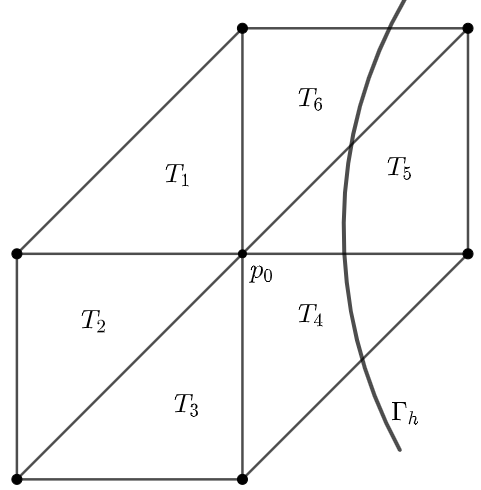
\includegraphics[width=0.4\linewidth]{metodocurvatura.png}
	\caption{Región cercana a $\Omega_h^\Gamma$ donde buscamos una aproximación $\kappa_h$ para la curvatura de $\Gamma_h$}.
	\label{fig:metodocurvatura}
\end{figure}
Si $D=\bigcup_{j=1}^6 T_j$ y $N_0\in \left\{ v\in C(D):\left.v\right\vert_T \in \mathbb{P}_1(T),\forall T \in D \right\}$ tal que $N_0(p_0)=1$ y $\left.N_0\right\vert_{\partial D}=0$ entonces
\[
\int_D\kappa_h N_0=\int_D N_0\nabla\cdot 	\left( \dfrac{\nabla \phi}{\|\nabla \phi \|}\right)
= -\int_D  	\left( \dfrac{\nabla N_0\cdot\nabla \phi}{\|\nabla \phi \|}\right)
\] de modo que el valor promedio de la curvatura es 
\begin{equation}
	\kappa_h(p_0) =-\frac{\dint_D  	\left( \dfrac{\nabla N_0\cdot\nabla \phi}{\|\nabla \phi \|}\right)}{\dint_D N_0}
	\label{eqn:curvaturaaproximacion}
\end{equation}
\begin{prop}[{\cite[p.~36]{shopple2009interface}}]
	Sea $\phi:\mathbb{R}^2\to \mathbb{R}$ y $p_0=(x_0,y_0)\in:\mathbb{R}^2$, $D=[x_0-h,x_0+h]\times [y_0-h,y_0+h]$ una región rectangular sobre la que se define una triangulación uniforme, es decir los vértices de los elementos están dados por $(x_0+ih,y_0+jh)$ para $i=-1,0,1$, $j=-1,0,1$. Si $N_0\in \left\{ v\in C(D):\left.v\right\vert_T \in \mathbb{P}_1(T),\forall T \in D \right\}$ tal que $N_0(p_0)=1$ y $\left.N_0\right\vert_{\partial D}=0$ y 
	\[
	\kappa_0 =-\left. \dint_D  	\left( \dfrac{\nabla N_0\cdot\nabla \phi}{\|\nabla \phi \|}\right)  \bigg/ \dint_D N_0 \right.\]
	entonces $\kappa_0$ aproxima la curvatura  de  $\Gamma=\{(x,y):\phi(x,y)=\phi(x_0,y_0)\}$ en el punto $p_0$ en el sentido de que
	\[
	\kappa_0 = \nabla\cdot 	\left( \dfrac{\nabla \phi}{\|\nabla \phi \|}\right) + O(h^2)\quad\text{y}\quad
	|\kappa_0 |\leqslant \frac{3\sqrt{2}}{h}
	\]
\end{prop}
Es posible construir una aproximación  $\kappa_h$ con polinomios cuadráticos al aplicar la ecuación \ref{eqn:curvaturaaproximacion} para encontrar $k_h(p)$ en  cada vértice $p$ de un refinamiento de la triangulación de $D$, como se muestra en la Figura \ref{fig:metodocurvaturarefinado}.
\begin{figure}[H]
	\centering
	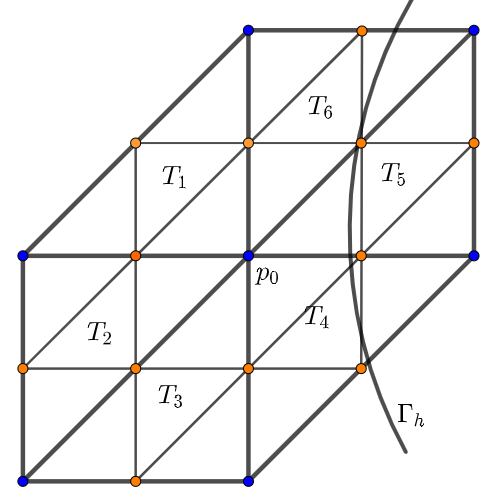
\includegraphics[width=0.4\linewidth]{metodocurvaturarefinado.png}
	\caption{Construcción de $\kappa_h$: Los vértices en color azul se utilizan en una aproximación por elementos de tipo $\mathbb{P}_1$ y los vértices de color naranja se utilizan en una aproximación de tipo $\mathbb{P}_2$.}
	\label{fig:metodocurvaturarefinado}
\end{figure}
%\[
%J(v)=\int_{\Omega_h^\Gamma} \left( v-\nabla \cdot \left( \dfrac{\nabla \phi}{\|\nabla \phi \|}\right)\right)^2
%\] y planteamos  el siguiente problema de mínimos cuadrados (\cite{mourad2005assumed}, \cite{chessa2003enriched}):
%\[
%J(\kappa_h)=\min_{v\in Q_h^{(1)}} J(v)
%\]

\comentario{
	Siguiendo a \citep{claus2019cutfem} y \citep{drz021}
	aproximamos la curvatura $\kappa$ por medio de $K_h$ perteneciente al espacio  $\mathcal{B}_h=\{v\in C^0(\Omega_\Gamma): v|_K\in P_1(K),\forall K\in \mathcal{T}_h\}$  y que es solución del siguiente problema: Encuentre $K_h\in \mathcal{B}_h$ tal que 
	
	\begin{equation}
		\int_{\Omega^\Gamma_h} K_h v + G_h(K_h,v) =
		\int_{\partial\Omega^\Gamma_h} (N_h\cdot n) v
		-
		\int_{\Omega^\Gamma_h} N_h\cdot \nabla v
		\quad,\forall v\in 
		\mathcal{B}_h
	\end{equation}
	donde
	\begin{equation}
		G_h(u,v)=\sigma h\sum_{e\in \mathcal{F}_h^\Gamma} \int_e \left[ n\cdot \nabla u\right]
		\left[ n\cdot \nabla v \right]
	\end{equation}
}
\section{Método de Características de Galerkin}
Una vez encontrada una extensión de la velocidad a todo el dominio fijo $\mathcal{O}$ podemos resolver la ecuación 	\ref{eqn:evolucionconjuntodenivel}
\[
\begin{aligned}	
	\frac{\partial \phi}{\partial t} + S(x,t)\cdot \nabla \phi =0,& \quad(x,t)\in\mathcal{O}\times \left(0,T\right] \\
	\phi(x,0)=\phi_0(x),&\quad x\in\mathcal{O}
\end{aligned}
\]
El método empleado es el de Características de Galerkin, para ello se divide el intervalo $[0,T]$ en $N$ subintervalos $[t_n,t_{n+1}]$ con $\Delta t=t_{n+1}-t_n$, luego las curvas características asociadas a la ecuación de advección son la solución del problema de valor inicial
\[
\begin{aligned}	
	\frac{d}{dt} X(t;x,t_{n+1})&=S(X(t;x,t_{n+1}),t),t\in [t_n,t_{n+1}] \\
	X(t_{n+1};x,t_{n+1}) &= x
\end{aligned}
\]
donde $X(t;x,t_{n+1})$ es el punto de partida de una partícula en el tiempo $t$ que llega a $x$ en el tiempo $t_{n+1}$, y
%\[
%X(t_n;x,t_{n+1})=x-\int_{t_n}^{t_{n+1}} %S(X(t;x,t_{n+1}),t) \,dt
%\]
por lo tanto a lo largo de las curvas características $\frac{d}{dt} \phi (X(t;x,t_{n+1}),t)=0$ entonces
\begin{equation}
	\phi (x,t_{n+1})=\phi (X(t_n;x,t_{n+1}),t_n) 
	\label{eqn:carac1}
\end{equation}
Para conocer el valor de $\phi (x,t_{n+1})$ es preciso tener una aproximación de $X(t_n;x,t_{n+1})$, por ello definimos $g(t)=\phi (X(t;x,t_{n+1}),t_n)$ con $x$, $t_n$, $t_{n+1}$ fijos, luego
\[
g(t-k)=g(t)+(-k)g'(t)+o(k^2)
\]
como $g'(t)=\nabla \phi (X(t;x,t_{n+1}),t_n)\cdot X'(t;x,t_{n+1})$ entonces para $t=t_{n+1}$ y $k=t_{n+1}-t_n$:
\[
g(t_n)=g(t_{n+1})-\Delta t\nabla \phi (X(t_{n+1};x,t_{n+1}),t_n)\cdot X'(t_{n+1};x,t_{n+1})+o((\Delta t)^2)
\]
vemos que $g(t_n)=\phi (X(t_n;x,t_{n+1}),t_n)$, 
$g(t_{n+1})=\phi (X(t_{n+1};x,t_{n+1}),t_n)=\phi (x,t_n)$, luego 
\[
\begin{aligned}
	\phi (X(t_n;x,t_{n+1}),t_n) &= \phi (x,t_n)
	-\Delta t\nabla \phi (X(t_{n+1};x,t_{n+1}),t_n)\cdot X'(t_{n+1};x,t_{n+1})+o((\Delta t)^2)\\
	& = \phi (x,t_n)
	-\Delta t\nabla \phi (x,t_n)\cdot X'(t_{n+1};x,t_{n+1})+o((\Delta t)^2)\\
	&= \phi (x,t_n) 
	-\Delta t\nabla \phi (x,t_n)\cdot 
	S(x,t_{n+1})+o((\Delta t)^2)
\end{aligned}
\]
Reemplazando en la ecuación \ref{eqn:carac1}:
\[
\phi (x,t_{n+1})=\phi (x,t_n) 
-\Delta t\nabla \phi (x,t_n)\cdot 
S(x,t_{n+1})+o((\Delta t)^2)
\]
también
\[
\phi (x-\Delta tS(x,t_{n+1}),t_{n})=
\phi (x,t_{n}) -\Delta t\nabla \phi (x,t_n)\cdot 
S(x,t_{n+1})+o((\Delta t)^2)
\]
por lo que
\begin{equation}
	\phi (x,t_{n+1})\approx \phi (x-\Delta tS(x,t_{n+1}),t_{n})
	\label{eqn:nuevophih}
\end{equation}
viene a ser una buena aproximación de $\phi (x,t_{n+1})$.

\section{Algoritmo para la evolución del crecimiento tumoral}
El algoritmo mostrado en la Figura \ref{eqn:algoritmo} contiene los pasos necesarios para aproximar la frontera del tumor en un tiempo $t=t_{max}$ cuando el crecimiento tumoral es aproximado  por medio de una discretización uniforme del dominio $\mathcal{O}$ en elementos triangulares y la función conjunto de nivel $\phi_h$  describe la frontera inicial del tumor. 

\begin{algorithm}[H]
	\SetKwInOut{Input}{Entrada}\SetKwInOut{Output}{Salida}
	\SetKwFor{Mientras}{Mientras}{hacer}{fin mientras}
	\Input{$\phi_h$, $\Delta t$, $t_{max}$}
	\Output{$p_h$, $c_h$, $\phi_h$ en tiempo $t_{max}$}
	\BlankLine
	$t\gets 0$.
	
	\Mientras{$t\leq t_{max}$}{
		Calcular $\kappa_h$ una aproximación de la curvatura en $\Omega_h^\Gamma$ por medio de la ecuación \ref{eqn:curvaturaaproximacion}.
		
		Calcular la concentración de nutrientes $c_h$ por medio de  la ecuación \ref{eqn:problemach}.
		
		Calcular  la presión intracelular $p_h$ por medio de la ecuación \ref{eqn:problemaph}.
		
		Calcular $V=(v_1,v_2)$ una aproximación de la velocidad de crecimiento tumoral en  $\Omega_h^\Gamma$ por medio  de la ecuación \ref{eqn:velocidadVn}.
		
		Calcular  $S_h=(S_{h,1},S_{h,2})$ la extensión de la velocidad $V$	 en el dominio fijo $\mathcal{O}$ por medio de la ecuación \ref{eqn:problemaSh}.
		
		Calcular  $\phi_h$ en tiempo $t+\Delta t$  por medio de la ecuación \ref{eqn:nuevophih}.
		
		$t\gets t+\Delta t$
	}
	\caption{Algoritmo para la simulación numérica de la evolución del crecimiento tumoral \label{eqn:algoritmo}}	
\end{algorithm}

\comentario{
	\section{Reinicialización de la función conjunto de nivel}
	Dada una función de conjunto de nivel $\phi_0$, el problema de reinicialización consiste en encontrar una nueva función conjunto de nivel $\phi$ que sea una función distancia dirigida respecto a la frontera libre $\Gamma=\left\{\phi_0=0\right\}$, es decir satisface  la ecuación eikonal o icónica
	\[
	|\nabla \phi|-1=0
	\]
	El método de reinicialización elíptica propuesto por \citep{basting2013minimization} y desarrollado en los trabajos de  \citep{adams2019high} y \citep{xue2021new}, consiste en resolver el problema de minimización
	\[
	\min_{\tilde{\phi}\in H^1(D)} \left(  R_3( |\nabla \tilde{\phi}| )\right)
	\]
	en un dominio $D\subset\mathcal{O}$ que contiene al dominio frontera, $\Omega_h^\Gamma \subset D$, y
	donde
	\[
	R_3( |\nabla \tilde{\phi}| ) = \int_D P_3(|\nabla \tilde{\phi}|)
	\]
	\[
	P_3( |\nabla \tilde{\phi}| ) = \begin{cases}
		\frac{1}{2}\left( |\nabla  \tilde{\phi}|-1\right)^2& ,
		|\nabla  \tilde{\phi}|>1 \\
		\frac{1}{3}\left( |\nabla  \tilde{\phi}|\right)^3
		-\frac{1}{2}\left( |\nabla  \tilde{\phi}|\right)^2
		+\frac{1}{6}& ,
		|\nabla  \tilde{\phi}|\leq 1 \\
	\end{cases}
	\]
	que conduce al siguiente problema de difusión casi lineal:
	\begin{align}
		\nabla \cdot \left( d_3\left(|\nabla \phi|\right)\nabla \phi \right) = 0,&\text{ en }D\\
		\phi =0, &\text{ en }\Gamma\\
		d_3\left(|\nabla \phi|\right)\nabla \phi \cdot n=0,&\text{ en }\partial D
	\end{align}
	donde el coeficiente de difusión $d_3$ esta definido como
	\begin{equation}
		d_3(s)=\begin{cases}
			1-\dfrac{1}{s}&,s>1\\
			s-1&,s\leq 1
		\end{cases}
	\end{equation}
	La ecuación casi lineal de difusión es resuelta en forma aproximada mediante la siguiente linealización con parámetro de penalización $\gamma>0$ para la condición Dirichlet: Encontrar $\phi \in H^1(D)$:
	\[
	\int_D \nabla \phi\cdot \nabla v  + \gamma \int_\Gamma \phi v=
	\int_D \left(1-d_3\left(|\nabla \phi|\right)\right)\nabla \phi\cdot  \nabla v,\forall v\in  H^1(D)
	\]
	que en el contexto del método de elementos finitos no ajustados a la frontera se aproxima como: Dados  $\phi^{n}, \phi_0\in \Phi_h$ encontrar  $\phi^{n+1}\in \Phi_h$, $p\in Q_h^{(l)}$ tal que
	\[
	\begin{aligned}
		\int_D \nabla \phi^{n+1}\cdot \nabla v  &+ \frac{\gamma}{h^2} \int_{\Omega_h^\Gamma} \left( \phi^{n+1}  - \frac{\phi_{0}}{h}p \right)\left( v  - \frac{\phi_{0}}{h}q \right)\\
		&+\sigma h \sum_{e\in \mathcal{F}_h^\Gamma} \int_e \left[ \frac{\partial \phi^{n+1}}{\partial n} \right]
		\left[ \frac{\partial v}{\partial n} \right]\\
		&=
		\int_D \left(1-d_3\left(|\nabla \phi^{n}|\right)\right)\nabla \phi^{n}\cdot  \nabla v,\forall v\in  \Phi_h,\forall q\in Q_h^{(l)}
	\end{aligned}
	\]
	\begin{align}
		a_{11}(u,v)=& \int_D \nabla u\cdot \nabla v 
		+	 \frac{\gamma}{h^2} \int_{\Omega_h^\Gamma} uv
		+ \sigma h \sum_{e\in \mathcal{F}_h^\Gamma} \int_e \left[ \frac{\partial u}{\partial n} \right]
		\left[ \frac{\partial v}{\partial n} \right] \\
		a_{12}(u,q)=& - \frac{\gamma}{h^3} \int_{\Omega_h^\Gamma} \phi_0 u q\\
		a_{21}(p,v)=&   - \frac{\gamma}{h^3} \int_{\Omega_h^\Gamma} \phi_0 pv\\
		a_{22}(p,q)=& \frac{\gamma}{h^4} \int_{\Omega_h^\Gamma} (\phi_{0})^2pq  \\	
		l(v)= & 
		\int_D \left(1-d_3\left(|\nabla \phi^{n}|\right)\right)\nabla \phi^{n}\cdot  \nabla v
	\end{align}
	%
	%\begin{align}
	%	\nabla \cdot \nabla \phi  =	\nabla \cdot \left( 1-d_3\left(|\nabla \phi|\right)\nabla \phi \right) ,&\text{ en }D\\
	%	\phi =0, &\text{ en }\Gamma\\
	%\nabla \phi \cdot n =	\left( 1 - d_3\left(|\nabla \phi|\right)\right)\nabla \phi \cdot n,&\text{ en }\partial D\\
	%\end{align}
	\subsection{Medidas del error}
	Si $\phi$ es solución del problema y $\phi_h$ es la solución del problema aproximado entonces definimos la siguientes medidas del error:
	\[
	\epsilon_{L^2}=\left( \int_D (\phi-\phi_h)^2 \right)^{1/2}
	\]
	\[
	\epsilon_{H^1}= \left( \int_D  |\phi-\phi_h|^2+|\nabla (\phi-\phi_h)|^2 \right)^{1/2}
	\]
	además podemos medir si la ecuación icónica es satisfecha
	\[
	\epsilon_{SD}= \left({\int_D (|\nabla \phi_h|-1)^2}
	\right)^{1/2}
	\]
	La medida del error en la aproximación de $\Gamma_h$ está dada por
	\[
	\epsilon_{Int}= \left({\int_{\Gamma_h} |\phi_h|^2}
	\right)^{1/2}
	\]
}
%\bibliography{levelset}	
\chapter{\MakeUppercase{Resultados numéricos}}
%\chapter{Resultados numéricos}
\thispagestyle{fancy}
El algoritmo  mostrado en la Figura \ref{eqn:algoritmo}   es implementado con el software FreeFEM++  \cite{MR3043640} que permite escribir la formulación variacional de los problemas que definen la concentración de nutrientes, la presión intracelular, la extensión de la velocidad y evolución de la función conjunto de nivel.
\section{Aproximación de un problema elíptico en un dominio circular}
En primer lugar analizamos la convergencia numérica de la solución del problema test
\begin{equation}
	-\Delta u+ u =f \text{ en } \Omega\quad
	u=\kappa \text{ en } \partial \Omega
	\label{eqn:problematest1}
\end{equation}
que tiene solución exacta $u_{ex}=\dfrac{1}{R^3}(x^2+y^2)$ cuando $\Omega=\{(x,y):x^2+y^2<R^2\}$. $\kappa(x,y)=\dfrac{1}{R}$ y $f = \dfrac{1}{R^3}(x^2+y^2-4)$.

Definimos $\phi=\sqrt{x^2+y^2}-R$ y elegimos como dominio fijo $\mathcal{O}=]-8,8[\times ]-8,8[$, el cual es discretizado de manera uniforme con $n=8(2^i)$ triángulos en la dirección horizontal y vertical para $i=2,3,4,5$

Las medidas del error son las siguientes: 
\[
\epsilon_{L^2}=\dfrac{\|u_h-u_{ex}\|_{0,\Omega_h\setminus\Omega_h^\Gamma}}{\|u_{ex}\|_{0,\Omega_h\setminus\Omega_h^\Gamma}}
\]
\[
\epsilon_{H^1}=\dfrac{|u_h-u_{ex}|_{1,\Omega_h\setminus\Omega_h^\Gamma}}{|u_{ex}|_{1,\Omega_h\setminus\Omega_h^\Gamma}}
\]
%\begin{defi}
%	Sea $p_n$ una sucesión tal que $p_n\to p$ y que $p_n \neq p$ para todo $n$. Si
%	\[
%	\lim_{n\to\infty} \frac{|p_{n+1}-p|}{|p_n-p|^\alpha}=\lambda
%	\]
%	entonces la sucesión converge a $p$ con orden $\alpha$ y constante de error asintótica $\lambda$.
%\end{defi}
%Para estimar el orden de convergencia de los métodos desarrollados, haremos la aproximación
%\[
%\frac{|p_{n+1}-p|}{|p_n-p|^\alpha}\approx \lambda \implies
%\log|p_{n+1}-p|\approx \alpha \log|p_n-p|  +  \log\log\lambda 
%\]
%por lo que una gráfica log-log puede ayudar a visualizar el orden de convergencia mediante la pendiente de la recta de los datos observados.

Si asumimos que $
\|u_h-u_{ex}\|\approx C  \|u_{ex}\|h^{\alpha}$ para algún $C>0$, entonces una gráfica log-log puede ayudar a visualizar un valor aproximado para $\alpha$ mediante la pendiente de la recta ajustada a los datos obtenidos, la cual será indicada en cada gráfica.

En las Figuras \ref{fig:convergenciaphifemdual1}, \ref{fig:convergenciaphifemdual2}, \ref{fig:convergenciaphifemdual3} se muestra la variación de  $\epsilon_{L^2}$ y $\epsilon_{H^1}$ respecto a $h$ cuando $k=1$, $k=2$ y $k=3$ respectivamente y haciendo variar $l=k,k+1,k+2$. En todos los casos el orden de convergencia $\alpha$ estimado es $k+1$ en la norma de $L^2$ y $k$ para la seminorma de $H^1$, es decir:
\[
\|u_h-u_{ex}\|_{0,\Omega_h\setminus\Omega_h^\Gamma}
\approx C  \|u_{ex}\|^{k+1}_{0,\Omega_h\setminus\Omega_h^\Gamma}
\]
\[
|u_h-u_{ex}|_{1,\Omega_h\setminus\Omega_h^\Gamma}
\approx C  |u_{ex}|^{k}_{1,\Omega_h\setminus\Omega_h^\Gamma}
\]

\begin{figure}[H]
	\centering
	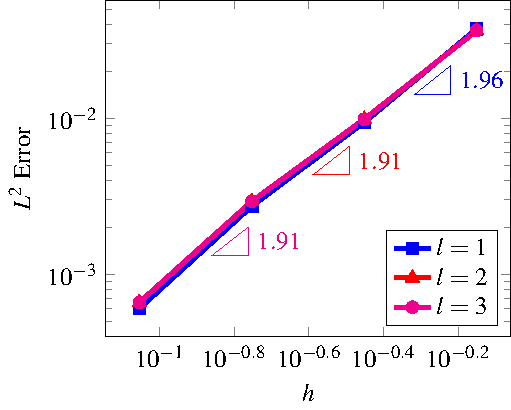
\includegraphics[width=0.4\linewidth]{img/convergenciaphifemdual1L2}\quad
	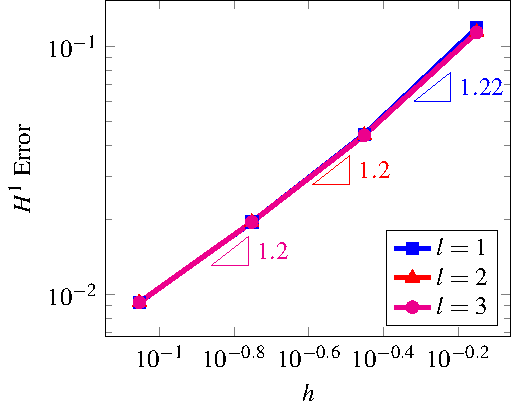
\includegraphics[width=0.4\linewidth]{img/convergenciaphifemdual1H1}
	\caption{Estimación del orden de convergencia  para la solución del problema mostrado en la ecuación \ref{eqn:problematest1} considerando $u_h\in V_h^{(1)}$,  y $\phi_h$ de tipo $\mathbb{ P}_l$. }
	\label{fig:convergenciaphifemdual1}
\end{figure}
\begin{figure}[H]
	\centering
	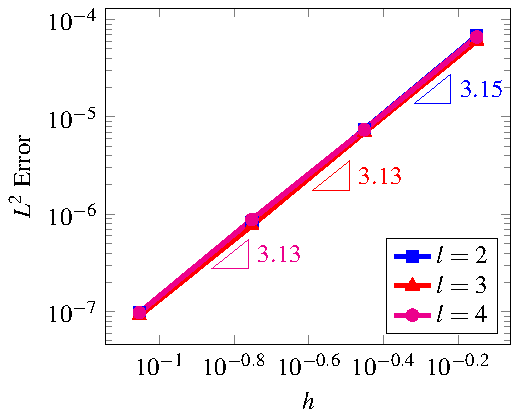
\includegraphics[width=0.4\linewidth]{img/convergenciaphifemdual2L2}\quad
	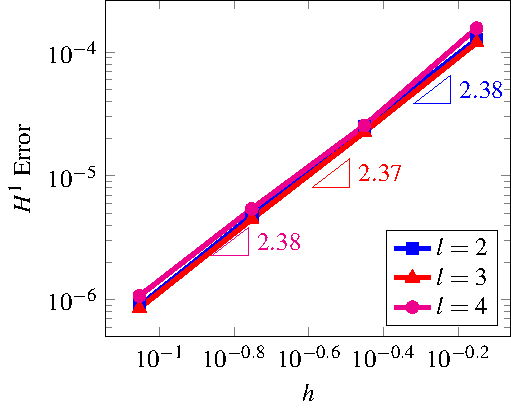
\includegraphics[width=0.4\linewidth]{img/convergenciaphifemdual2H1}
	\caption{Estimación del orden de convergencia  para la solución de la ecuación \ref{eqn:problematest1} considerando $u_h\in V_h^{(2)}$,  y $\phi_h$ de tipo $\mathbb{ P}_l$. }
	\label{fig:convergenciaphifemdual2}
\end{figure}

\begin{figure}[H]
	\centering
	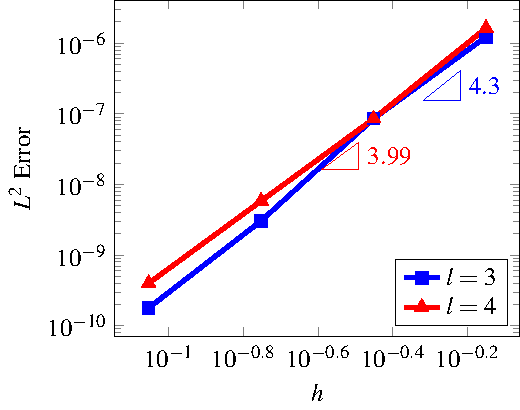
\includegraphics[width=0.4\linewidth]{img/convergenciaphifemdual3L2}\quad
	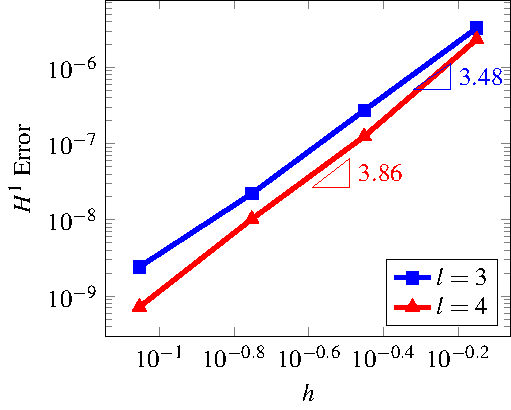
\includegraphics[width=0.4\linewidth]{img/convergenciaphifemdual3H1}
	\caption{Estimación del orden de convergencia  para la solución de la ecuación \ref{eqn:problematest1} considerando $u_h\in V_h^{(3)}$,  y $\phi_h$ de tipo $\mathbb{ P}_l$. }
	\label{fig:convergenciaphifemdual3}
\end{figure}
\section{Aproximación de la curvatura para el caso de un tumor con frontera circular}
Si consideramos que la curvatura de $\Gamma_h$ puede aproximarse por la ecuación \ref{eqn:curvaturaaproximacion} entonces el orden de convergencia estimado es $k+1$ en la norma de $L^2$ y $k$ para la seminorma de $H^1$, tal como se aprecia en la Figura  \ref{fig:convergenciaphifemdualcurvatura}.

\begin{figure}[H]
	\centering
	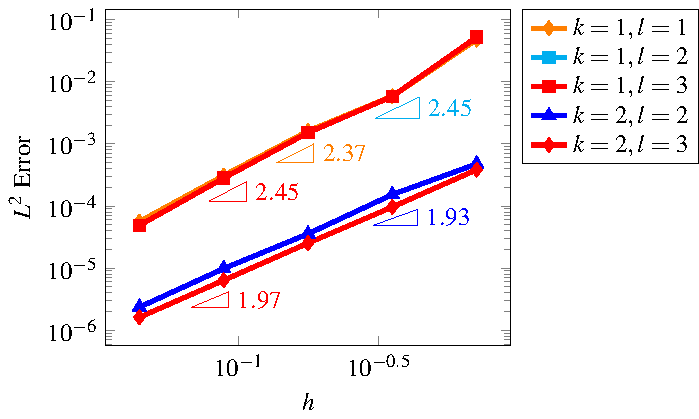
\includegraphics[width=0.6\linewidth]{img/convergenciaphifemdualcurvaturaL2}\quad
	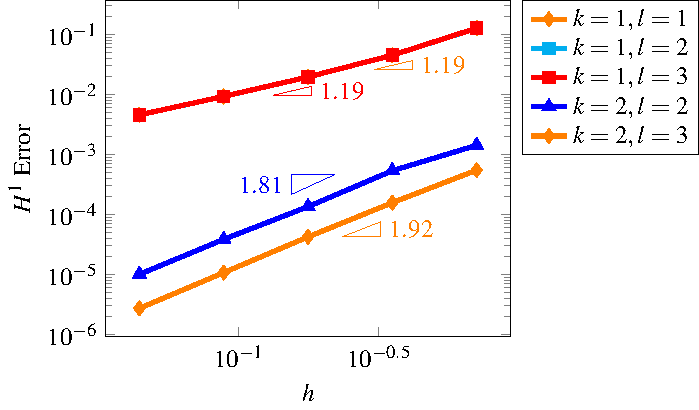
\includegraphics[width=0.6\linewidth]{img/convergenciaphifemdualcurvaturaH1}	
	\caption{Estimación del orden de convergencia  para la solución del problema \ref{eqn:curvaturaaproximacion} considerando $u_h\in V_h^{(k)}$,  y $\phi_h$ consta de elementos de tipo $\mathbb{ P}_l$.}
	\label{fig:convergenciaphifemdualcurvatura}
\end{figure}
\comentario{
	Para el caso del cálculo de la presión intracelular el problema \ref{eqn:phifemdual} se escribe como
	\begin{equation}
		\begin{aligned}
			\int_{\Omega_h}\nabla w \cdot \nabla v
			- \int_{\partial \Omega_h} \frac{\partial w}{\partial n}  v
			+ \frac{\gamma}{h^2}  \int_{\Omega_h^\Gamma} (w-\frac{1}{h}\phi_h p) (v-\frac{1}{h}\phi_h q)
			+G_h(w,v)+J_h^{lhs}(w,v)
			=\\
			\frac{\gamma}{h^2}  \int_{\Omega_h^\Gamma} \kappa_h (v-\frac{1}{h}\phi_h q)+J_h^{rhs}(v)
		\end{aligned}
	\end{equation}
	Es posible escribir el término $ \int_{\Omega_h^\Gamma} \kappa_h (v-\frac{1}{h}\phi_h q)$ como
	\[
	\int_{\Omega_h^\Gamma} \nabla\cdot\left(\frac{\nabla\phi_h}{|\nabla\phi_h|}\right) (v-\frac{1}{h}\phi_h q)= \int_{\partial\Omega_h^\Gamma} (v-\frac{1}{h}\phi_h q) \left(\frac{\nabla\phi_h}{|\nabla\phi_h|}\right)\cdot n
	- \int_{\Omega_h^\Gamma} \left(\frac{\nabla\phi_h}{|\nabla\phi_h|}\right) \cdot \nabla(v-\frac{1}{h}\phi_h q)
	\]
	Este cambio solo afecta al lado derecha de la ecuación así que el problema sigue teniendo solución única.
	
	
	En la Figura \ref{fig:convergenciacurvaturacirculo} se muestra el error cometido sobre la frontera $\Gamma_h$ cuando aproximamos la curvatura por $K_h$ para el caso de las curvas polares $r=4$ y $r=2.1 + 0.5\cos(2t)$ en un dominio global $\mathcal{O}=\left]-3,3\right[^2$. La curvatura para una curva polar $r=f(\theta)$ está dada por
	\[
	\kappa =\frac{2(f'(\theta))^2+(f(\theta))^2-f(\theta)f''(\theta)}{
		\left[
		(f'(\theta))^2+(f(\theta))^2
		\right]^{3/2}
	}
	\]
	y el error cometido en la aproximación esta definido por
	\[
	\epsilon_h =\|\kappa - K_h\|_{L^2(\Gamma_h)}
	\]
	así hemos encontrado una extensión suave de la curvatura definida sobre el dominio banda $\Omega_h$.
}
\section{Extensión de la velocidad definida sobre una interfase circular}
Consideremos el problema de interfase circular propuesto en \cite{utz2018high}: el dominio fijo es $\mathcal{O}=\left<-2,2\right>^2 \setminus [-\frac{1}{2},\frac{1}{2}]^2$ y la función conjunto de nivel es $\phi(x,y)=\sqrt{x^2+y^2}-1$ de manera que la interfase $\Gamma$ esta definida por $\left\{(x,y):\phi(x,y)=0\right\}$. Consideramos $u_0:\Gamma \to\mathbb{R}$ tal que 
\[
u_0(x,y)=1-x^2+y
\]
Como la rectas que contienen al origen, con ángulo de inclinación $\theta$ son normales a la interfase entonces la extensión $u:\mathcal{O}\to\mathbb{R}$ debe satisfacer que
\[
\begin{aligned}
	u(x,y) &= u_0(\cos \theta, \sen \theta)=1-\cos^2\theta  +\sen\theta \\
	&=1-\frac{x^2}{x^2+y^2}+\frac{y}{\sqrt{x^2+y^2}}\\
	&=y\left(\frac{y+\sqrt{x^2+y^2}}{\sqrt{x^2+y^2}}
	\right)
\end{aligned}
\]
Para estimar el orden de convergencia de la solución del problema \ref{eqn:problemaextension} se utilizan $2n^2$ elementos tipo $\mathbb{P}_k$, con $n=8\cdot 2^i$ para $i=2,3,4,5$ y $h=4\sqrt{2}/n$, los resultados se muestran en la Figura \ref{fig:convergenciaextension} considerando $k=1$, $k=2$, $k=3$. Así el orden de convergencia estimado en la norma $L^2$ es $k+1$ y en la norma $H^1$ es $k$.
\begin{figure}[H]
	\centering
	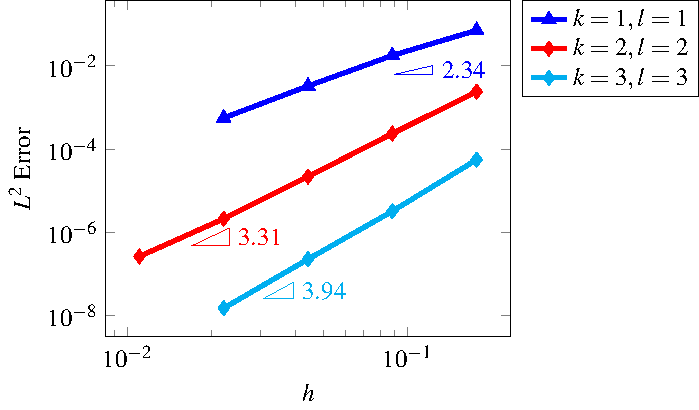
\includegraphics[width=0.6\linewidth]{img/convergenciaextensionL2}\quad
	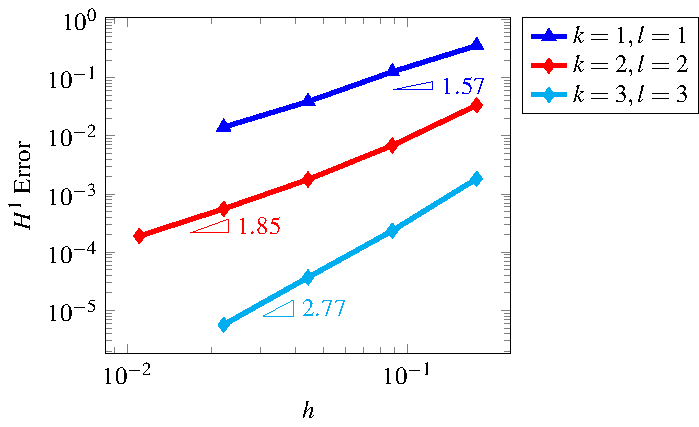
\includegraphics[width=0.6\linewidth]{img/convergenciaextensionH1}	
	\caption{Estimación del orden de convergencia  para la solución del problema \ref{eqn:problematest1} considerando $u_h\in V_h^{(k)}$, y $\phi_h$  de tipo $\mathbb{ P}_l$.}
	\label{fig:convergenciaextension}
\end{figure}
A continuación se calcula la extensión de la velocidad considerando elementos $\mathbb{P}_2$ triangulares $h=0.176777$ y  $n=32$,  sobre un mallado uniforme del dominio fijo $\mathcal{O}$. Como se observa en la Figura \ref{fig:extensioncurvas} las curvas de nivel de la extensión de la velocidad son ortogonales a la interfase circular, de igual modo en la Figura \ref{fig:extensionerror} se muestra como el error $u-u_h$ se propaga a través de las curvas de nivel de la extensión de la velocidad.
\begin{figure}[H]
	\centering
	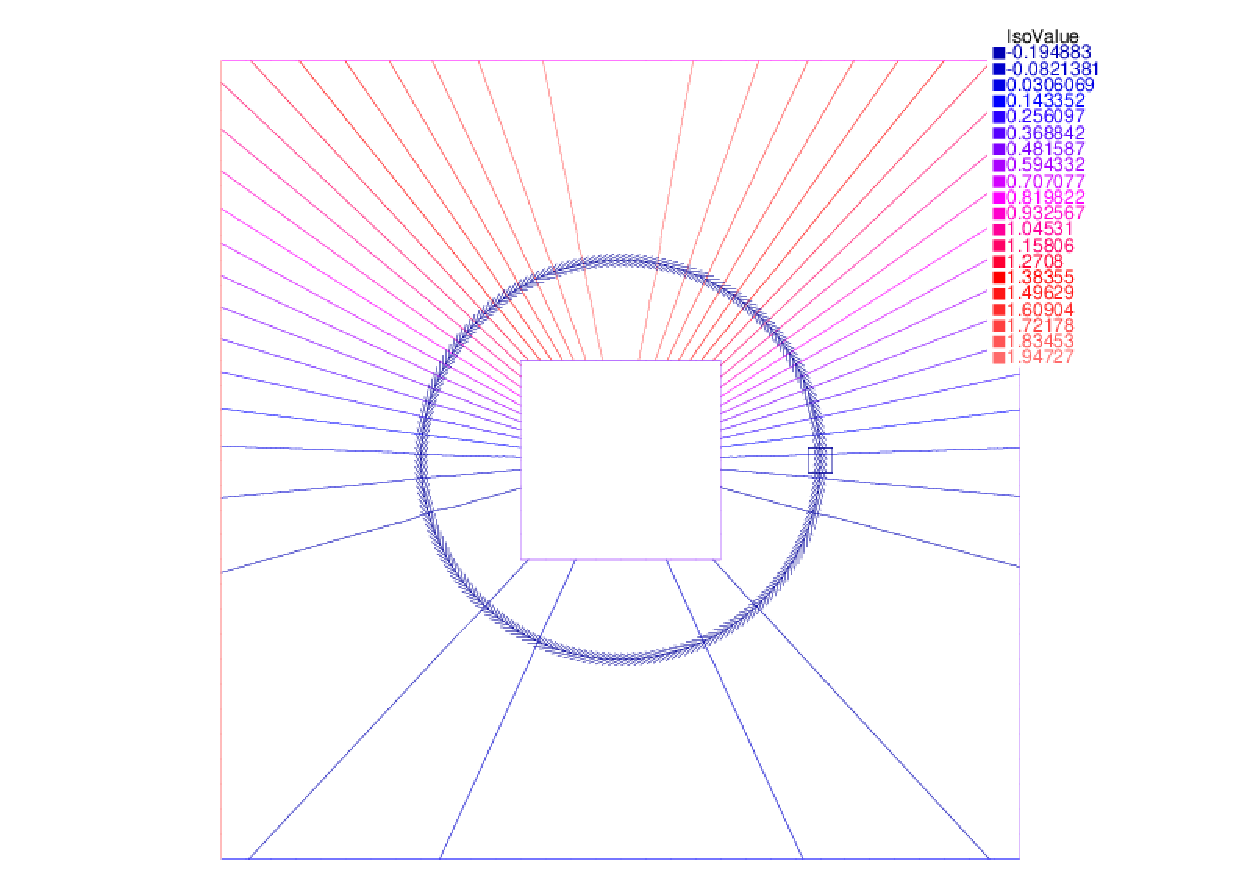
\includegraphics[width=0.7\linewidth]{img/extensioncurvas}	
	\caption{Curvas de nivel para la extensión de la velocidad en el caso de un interfase circular.}
	\label{fig:extensioncurvas}
\end{figure}
\begin{figure}[H]
	\centering
	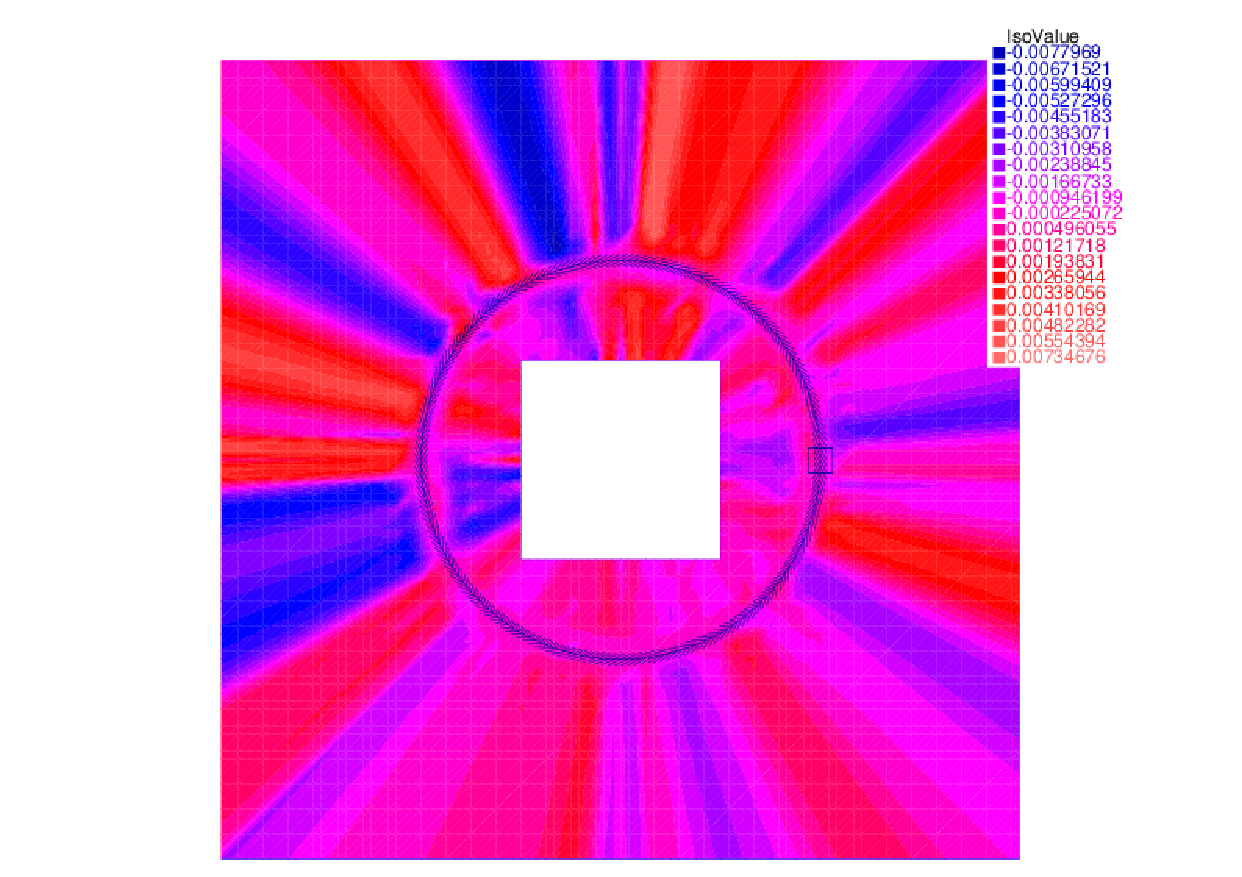
\includegraphics[width=0.7\linewidth]{img/extensionerror}
	\caption{Error de la aproximación de la extensión: $u-u_h$ para $k=l=2$ (elementos $\mathbb{ P}_2$)}
	\label{fig:extensionerror}
\end{figure}
\section{Extensión de la velocidad definida sobre una interfase no circular}
Consideremos la función conjunto de nivel $\phi(x,y)=x+x|y|$ de modo que la interfase $\Gamma$ corresponde con la recta vertical $x=0$, y tenemos $u_0:\Gamma \to\mathbb{R}$ una función que deseamos extender a una función $u:\Omega \to\mathbb{R}$ tal que $\Gamma\subset\Omega$ y $\Gamma \subset \Omega$. Para ello aplicamos el método de curvas características:
\[
\partial_x\phi(x,y) = 1+|y|, \text{si }x,y\in\mathbb{R}
\]
\[
\partial_y\phi(x,y) = \begin{cases}
	x,& \text{si }x\in\mathbb{R},y>0\\
	-x,& \text{si }x\in\mathbb{R},y<0\\
	0,& \text{si }x=0,y=0
\end{cases}
\]

luego una curva característica $\alpha$ está definida por la ecuaciones
\[
x'(t)=1+|y(t)|,\quad y'(t)=x
\]
\begin{figure}[H]
	\centering
	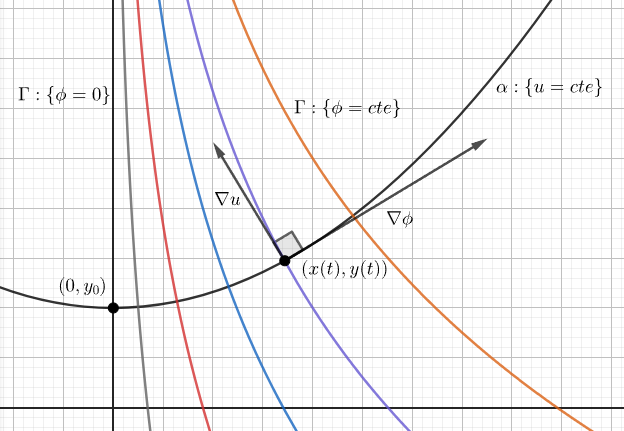
\includegraphics[width=0.7\linewidth]{img/extension}	
	\caption{Curvas características para la extensión de la velocidad cuando la interfase coincide con el eje $y$.}
	\label{fig:extensionnocircular}
\end{figure}
Si $y_0>0$ entonces $y(t)>0$, luego
\[
\frac{dy}{dt}=\frac{dy}{dx}\frac{dx}{dt}=\frac{dy}{dx}(1+y)=x
\]
integrando tenemos que
\[
2y+y^2 = x^2 + C
\]
y por la condición inicial $y(0)=y_0$, $x(0)=0$
\[
2y+y^2 = x^2 + 2y_0+y_0^2
\]
de donde 
\[
y_0 = \sqrt{(1+y)^2-x^2}-1
\]
de igual manera para $y_0<0$
\[
y_0 = 1-\sqrt{(1-y)^2-x^2}
\]
y como en la curva característica el valor de $u$ es constante, $u(x,y)=u(0,y_0)=u_0(y_0)$:
\[
u(x,y)=
\begin{cases}
	u_0(\sqrt{(1+y)^2-x^2}-1),&y>\sqrt{1+x^2}-1\\
	u_0(1-\sqrt{(1-y)^2-x^2}),&y<1-\sqrt{1+x^2}
\end{cases}
\]
Lo cual quiere decir que en la región donde $1+|y|<\sqrt{1+x^2}$ el problema está mal puesto y se tendrán resultados espurios al resolver la ecuación \ref{eqn:problemaSh}  con $\epsilon=0$, dicha perdida de regularidad se observa la Figura \ref{fig:extensionnocircular3d}; sin embargo considerando la Proposición \ref{prop:extension} con 
$\epsilon=10^{-2}$ garantizamos la existencia de solución única para el problema de extensión,  aunque ya no se tendrá la propagación de los valores de la interfase a través de las curvas de nivel tal como se observa en la Figura \ref{fig:extensionnocircularniveles}.

\begin{figure}[H]
	\centering	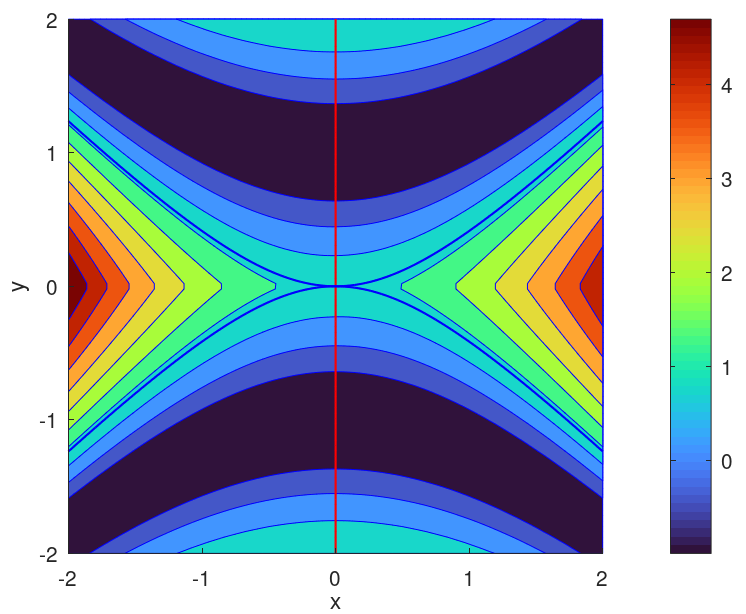
\includegraphics[width=0.6\linewidth]{img/extension1}	 \quad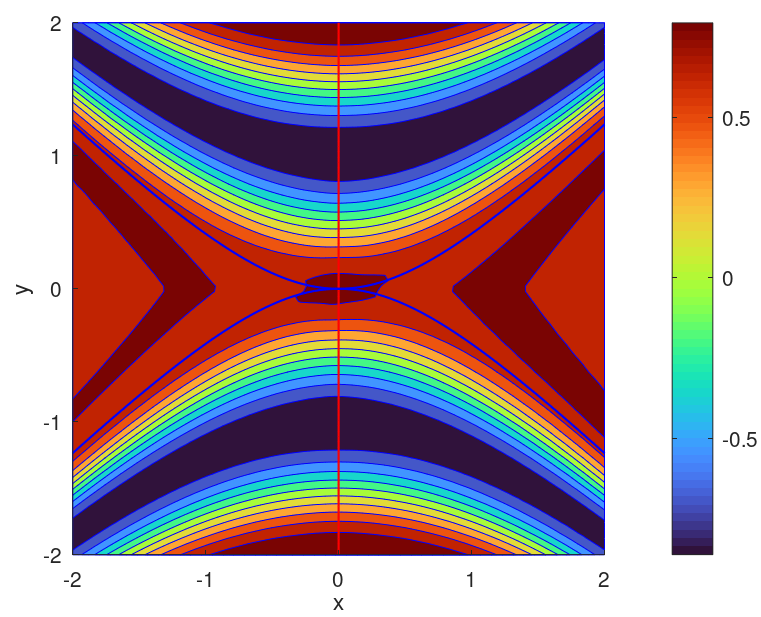
\includegraphics[width=0.6\linewidth]{img/extension2}
	\caption{Curvas de nivel para la extensión de la velocidad. Arriba: solución con $\epsilon=0$. Abajo:  solución con $\epsilon=10^{-2}$}	\label{fig:extensionnocircularniveles}
\end{figure}
\begin{figure}[H]
	\centering	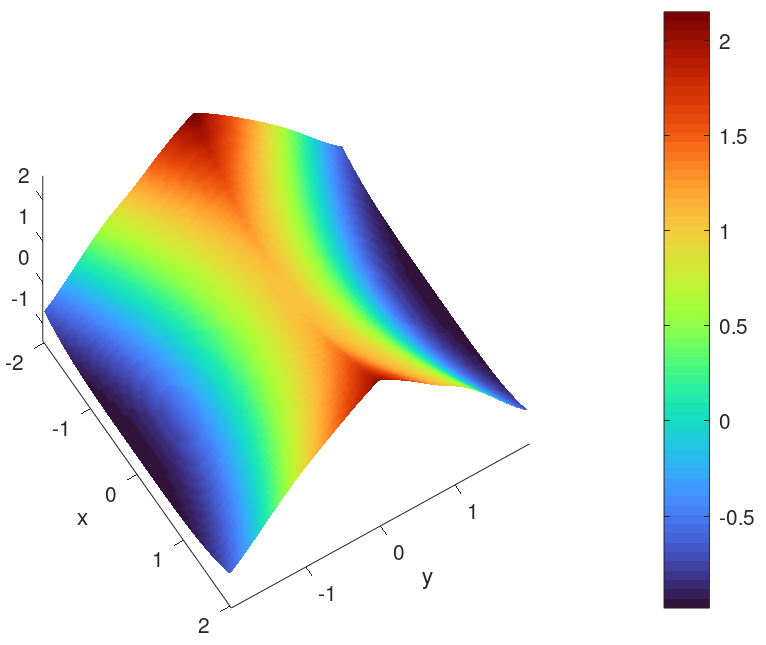
\includegraphics[width=0.6\linewidth]{img/extension3d1}	 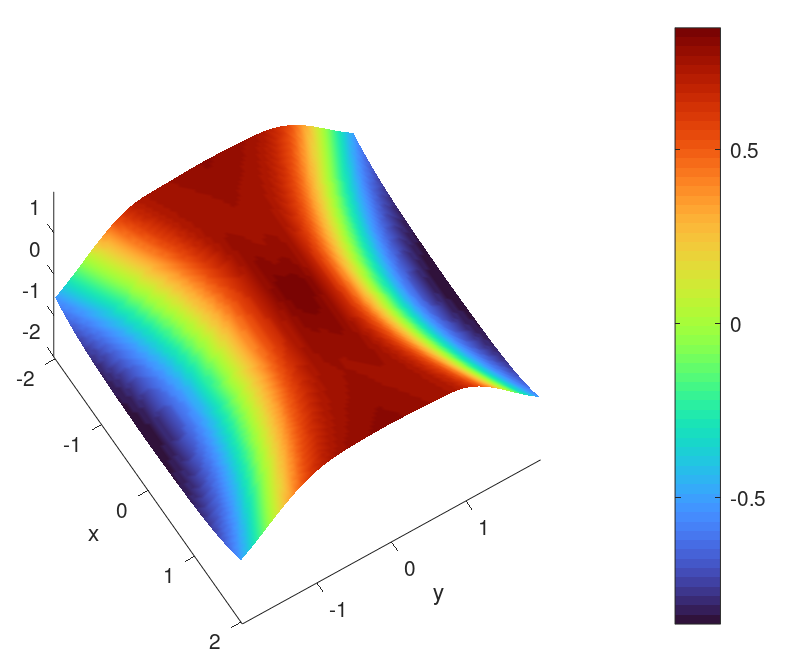
\includegraphics[width=0.6\linewidth]{img/extension3d2}
	\caption{Vista tridimensional de la extensión de la velocidad. Arriba: solución con $\epsilon=0$. Abajo:  solución con $\epsilon=10^{-2}$}	\label{fig:extensionnocircular3d}
\end{figure}
\section{Rotación de un dominio circular definido por una curva de nivel}
Consideremos $\phi_0(x,y)=\sqrt{(x-1)^2+y^2}-1$ y el campo de velocidades $(v_1,v_2)=(y,-x)$, con dominio fijo $\mathcal{O}=\left]-4,4\right[^2$. La interfase $\Gamma(t)$ esta definida por $\{(x,y):\phi(x,y,t)=0\}$ de modo que la ecuación de evolución de la función conjunto de nivel es
\[
\partial_t \phi + y\phi_x - x\phi_y=0
\]
Siguiendo el método de características, si $x(t),y(t)$ es tal que $\phi(x(t),y(t),t)=0$ entonces
\[
x'(t)=y(t)\quad y'(t)=-x(t)
\]
por lo tanto se se satisface el siguiente sistema desacoplado de EDO's
\begin{equation}
	\begin{aligned}
		x''(t)+x(t)=&0 \\
		y''(t)+y(t)=&0
	\end{aligned}
	\label{eqn:edo}
\end{equation}
además
\[
\frac{d}{dt}(x(t)^2+y(t)^2)=2(x'(t)x(t)+y'(t)y(t))=0
\]
lo cual indica que las curvas características son circunferencias centradas en el origen de radio $r=\sqrt{x_0^2+y_0^2}$.

Entonces la solución del sistema de EDO's (\ref{eqn:edo}) es \[
x(t)=x_0\cos t - y_0\sen t, \quad y(t)=x_0\sen t + y_0\cos t
\]

Al aplicar el método de aproximación por características de Galerkin (\ref{eqn:nuevophih}), considerando 2048 elementos triangulares $\mathbb{P}_2$ y $h=0.353553$ obtenemos la evolución de la interfase para $t=0, \frac{\pi}{2},\pi, \frac{3\pi}{2},2\pi$, como se muestra en la Figura \ref{fig:rotacion}.
\begin{figure}[H]
	\centering
	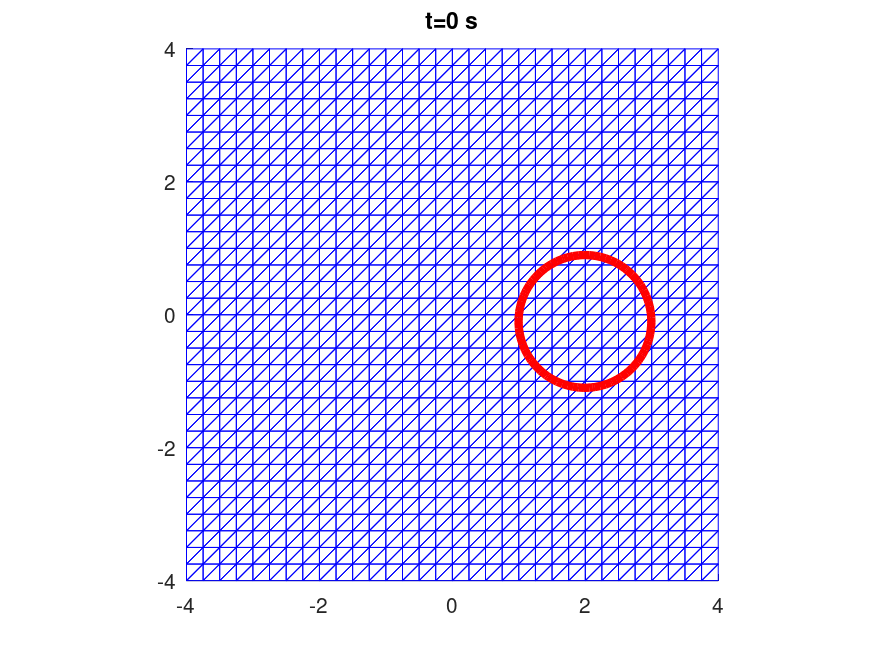
\includegraphics[width=0.4\linewidth]{img/rotacion1}
	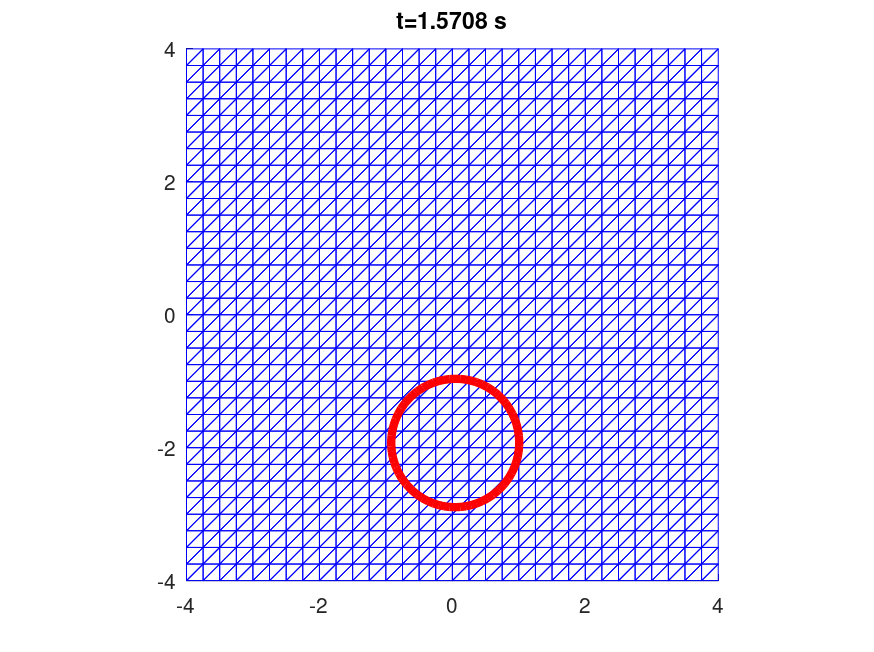
\includegraphics[width=0.4\linewidth]{img/rotacion2}
	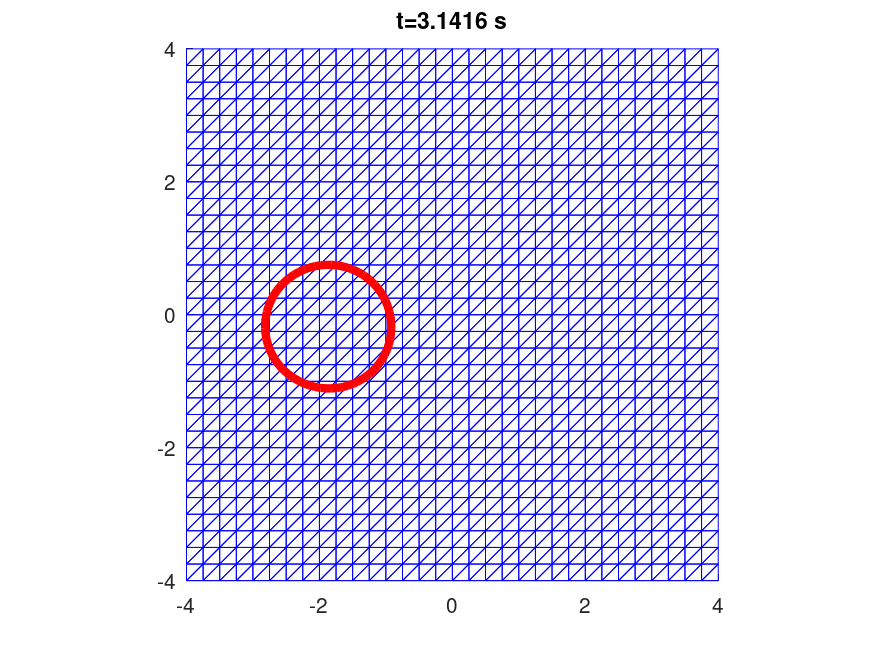
\includegraphics[width=0.4\linewidth]{img/rotacion3}
	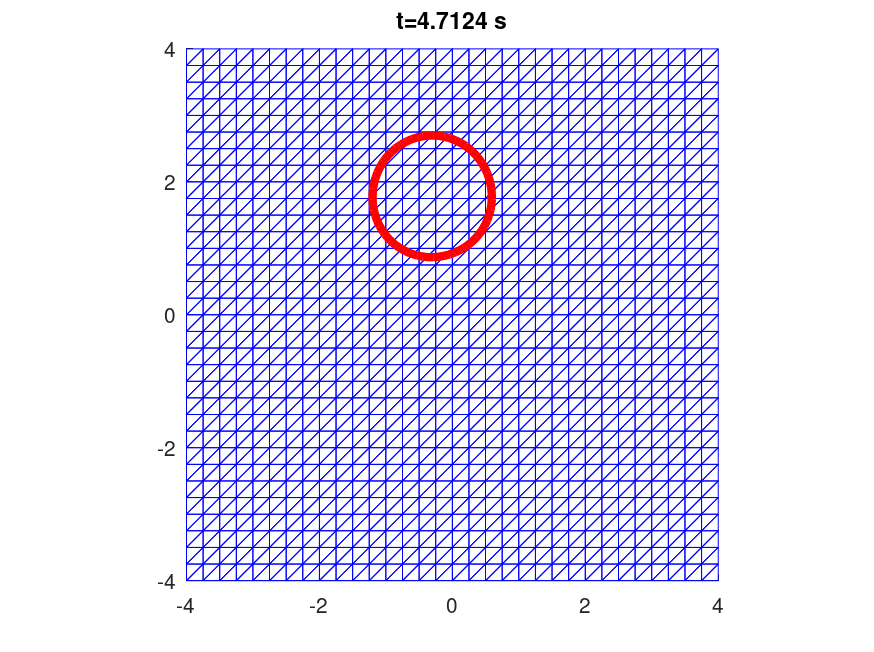
\includegraphics[width=0.4\linewidth]{img/rotacion4}
	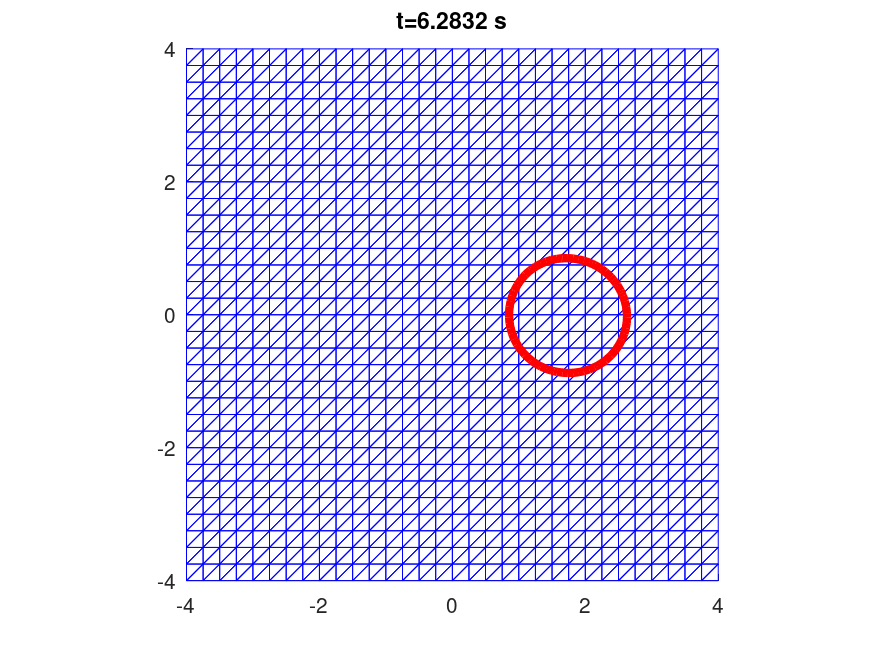
\includegraphics[width=0.4\linewidth]{img/rotacion5}
	\caption{Evolución de la interfase circular $\Gamma(t)$ si  $\Gamma(0):=\{(x,y):\phi_0(x,y)=0\}$}
	\label{fig:rotacion}
\end{figure}


\section{Solución exacta del crecimiento tumoral con simetría radial}
En este caso simulamos la evolución del crecimiento de un tumor con frontera inicial circular en etapa de baja vascularización y que por lo tanto se acerca a la solución estacionaria con radio $R_\infty$ dado por la ecuación \ref{eqn:radioestacionario}. Escogemos los parámetros 
$R(t=0)=4$, $A=1/2$, $G=20$, de modo que 
\[
2.8284\approx \sqrt{8}<R_\infty <4
\]
Los valores mostrados en el cuadro \ref{tabla:solucioncircular} son  calculados al resolver numéricamente la ecuación \ref{eqn:edoradiotumor} por medio del método de Adams predictor-corrector implementado por la librería LSODE parte de ODEPACK  \footnote{\url{https://computing.llnl.gov/projects/odepack}}  \cite{radhakrishnan1993description}. 
\begin{table}[H]
	\footnotesize
	\centering
	\caption{Velocidad de crecimiento en la frontera de un tumor con simetría circular de radio $R$.}
	\label{tabla:solucioncircular}
	\begin{tabular}{ccc}
		\toprule
		$t$&$V(t)$&$R(t)$ \\
		\midrule
		0  &-2.7295  & 4.0000 \\
		0.1000 & -1.7979 &  3.7771\\
		0.2000 & -1.1957 &  3.6295\\
		0.3000 & -0.8010 &  3.5310\\
		0.4000 & -0.5395 &  3.4649\\
		0.5000 & -0.3648 &  3.4203\\
		0.6000 & -0.2473 &  3.3900\\
		0.7000 & -0.1680 &  3.3695\\
		0.8000 & -0.1142 &  3.3556\\
		0.9000&  -0.0778 &  3.3461\\
		1.0000 & -0.0530 &  3.3397\\
		\bottomrule
	\end{tabular}
	
\end{table}
En las Figuras \ref{fig:crecimientoa05R04}-\ref{fig:crecimientoa05R02} se muestra el comportamiento del radio del tumor así como la velocidad en la frontera, y se observa que se estabilizan alrededor de la solución estacionaria asociada a $R_\infty$.
\begin{figure}[H]
	\centering
	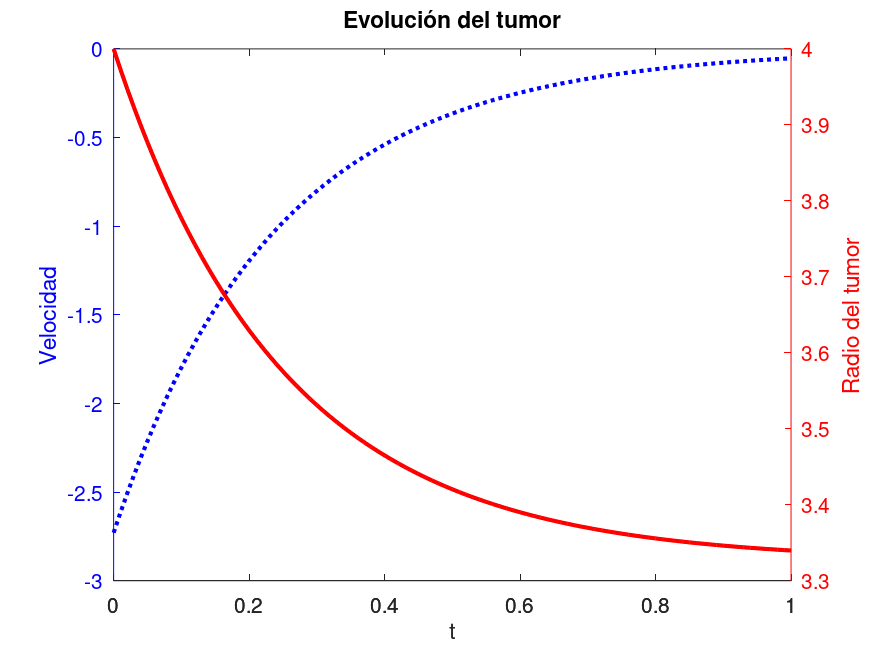
\includegraphics[width=0.7\linewidth]{crecimientoa05R04}
	\caption{Solución numérica de la ecuación \ref{eqn:edoradiotumor} con los parámetros $R_0=4$, $A=0.5$, $G=20$.}
	\label{fig:crecimientoa05R04}
\end{figure}
\begin{figure}[H]
	\centering
	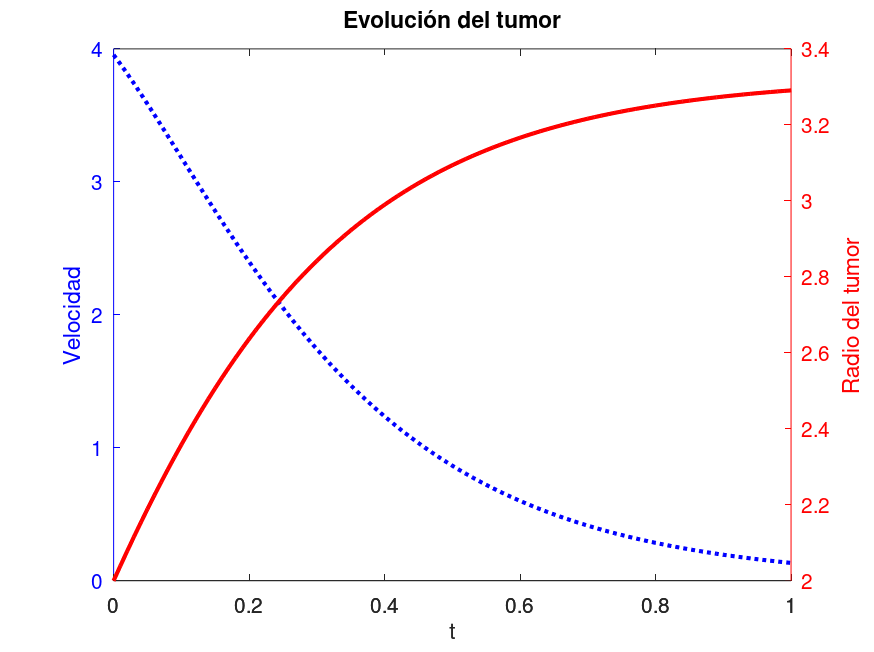
\includegraphics[width=0.7\linewidth]{crecimientoa05R02}
	\caption{Solución numérica de la ecuación \ref{eqn:edoradiotumor} con los parámetros $R_0=2$, $A=0.5$, $G=20$}
	\label{fig:crecimientoa05R02}
\end{figure}

En el caso que $A\geq 1$ y $G>0$ tenemos que
\[
-\frac{A}{2}<\frac{1}{w_0}-\frac{A}{2}<\frac{1-A}{2}\leq 0\implies V< 0
\]
por lo que $R$ es decreciente, y el tumor tiende a extinguirse como se aprecia en  la Figura \ref{fig:crecimientoa1dot5g20}.

\begin{figure}[H]
	\centering
	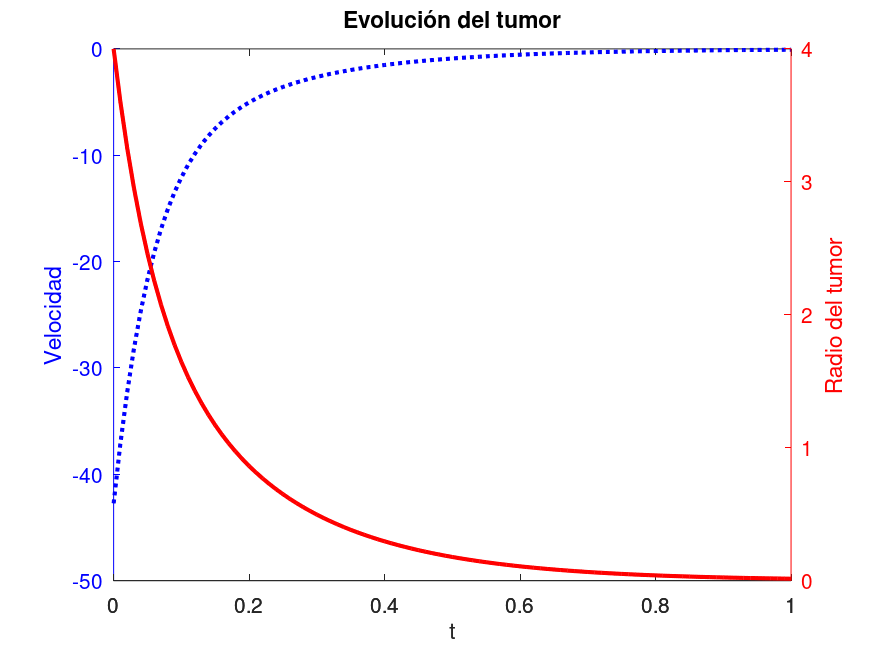
\includegraphics[width=0.7\linewidth]{crecimientoa1dot5G20}
	\caption{Solución numérica de la ecuación \ref{eqn:edoradiotumor} con los parámetros $A=1.5$, $G=20$}
	\label{fig:crecimientoa1dot5g20}
\end{figure}

\begin{figure}[H]
	\centering
	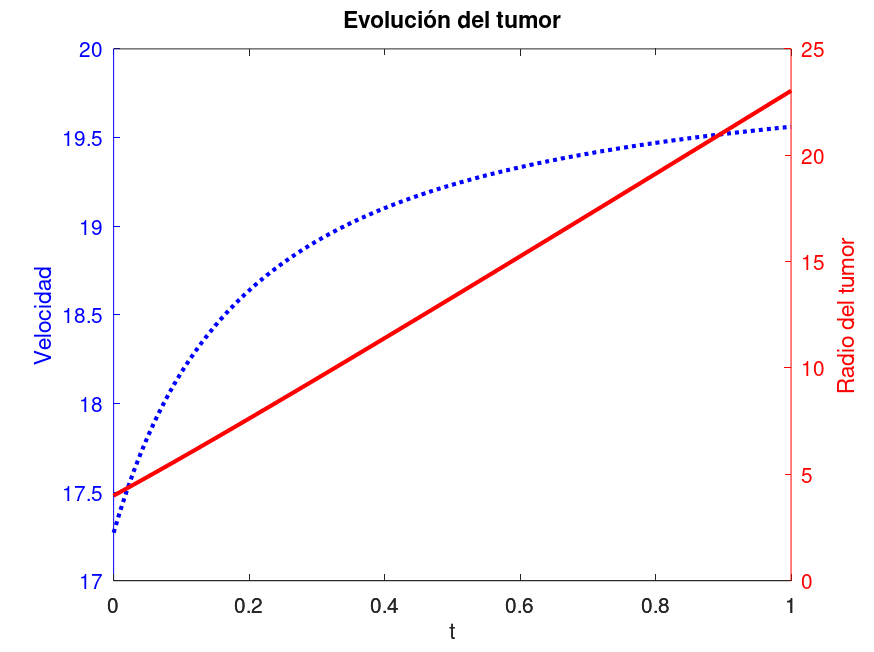
\includegraphics[width=0.7\linewidth]{crecimientoa0}
	\caption{Solución numérica de la ecuación \ref{eqn:edoradiotumor} con los parámetros $R_0=4$, $A=0.0$, $G=20$}
	\label{fig:crecimientoa0}
\end{figure}
\begin{figure}[H]
	\centering
	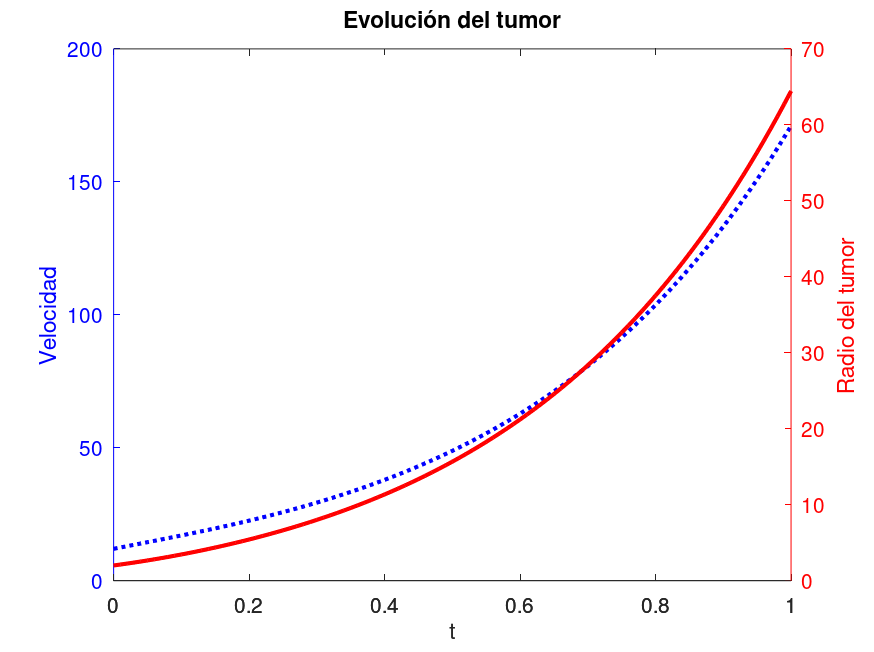
\includegraphics[width=0.7\linewidth]{crecimientoa-05G10}
	\caption{Solución numérica de la ecuación \ref{eqn:edoradiotumor} con los parámetros $R_0=2$, $A=-0.5$, $G=10$}
	\label{fig:crecimientoa-05G10}
\end{figure}
\section{Experimentos numéricos para el crecimiento de un tumor no circular} 
En las Figuras \ref{fig:evolucionnutrientesA}-\ref{fig:evolucionpresionA} los valores que identifican el régimen de baja vascularidad son $G=20$, $A=0.5$ y la frontera inicial del tumor está dada por la curva polar 
\begin{equation}
	r=2.1+0.5\cos(2\theta)
	\label{eqn:casoA}
\end{equation}
\begin{figure}[H]
	\centering
	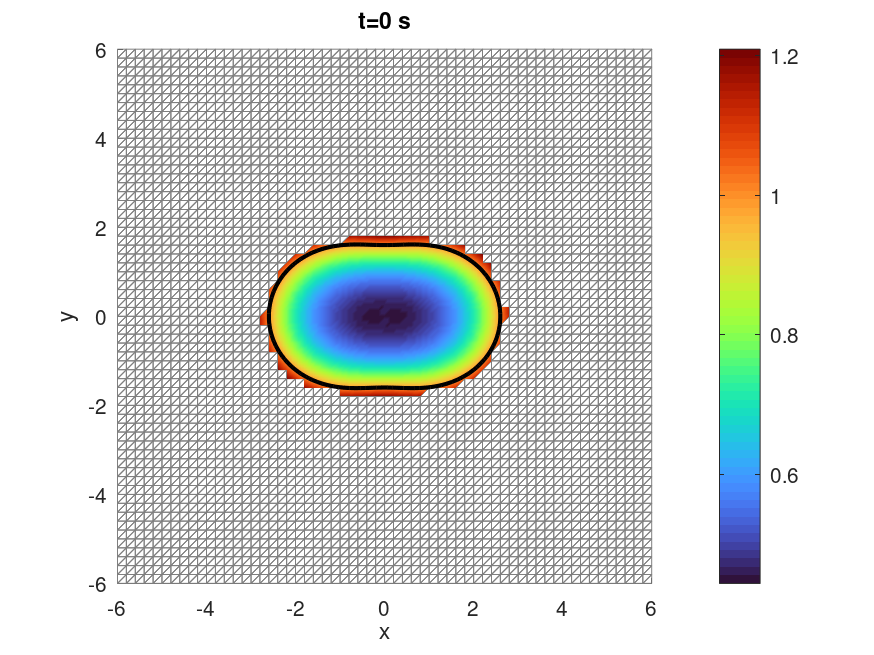
\includegraphics[width=0.4\linewidth]{casoA/nutrientes0}
	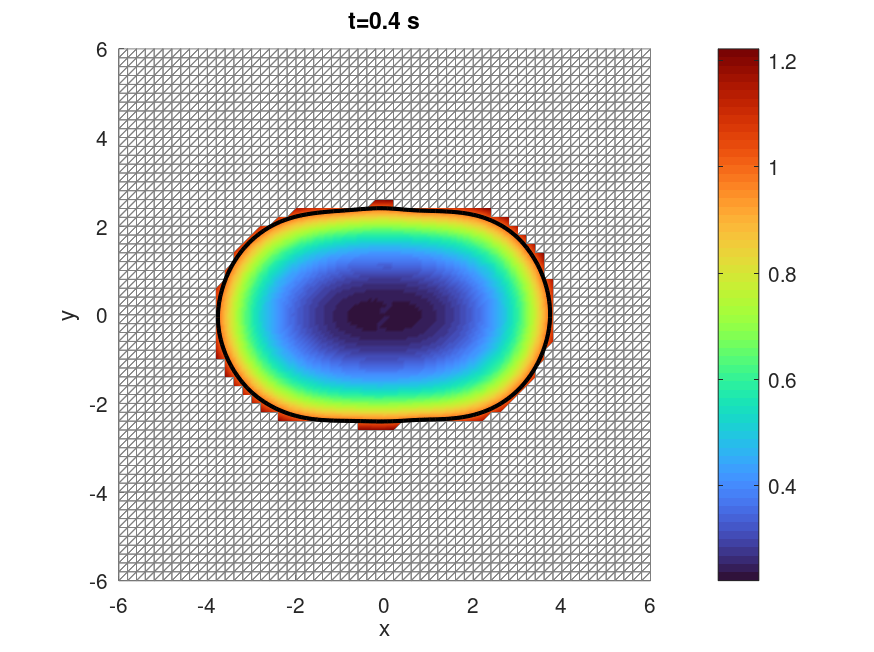
\includegraphics[width=0.4\linewidth]{casoA/nutrientes400}
	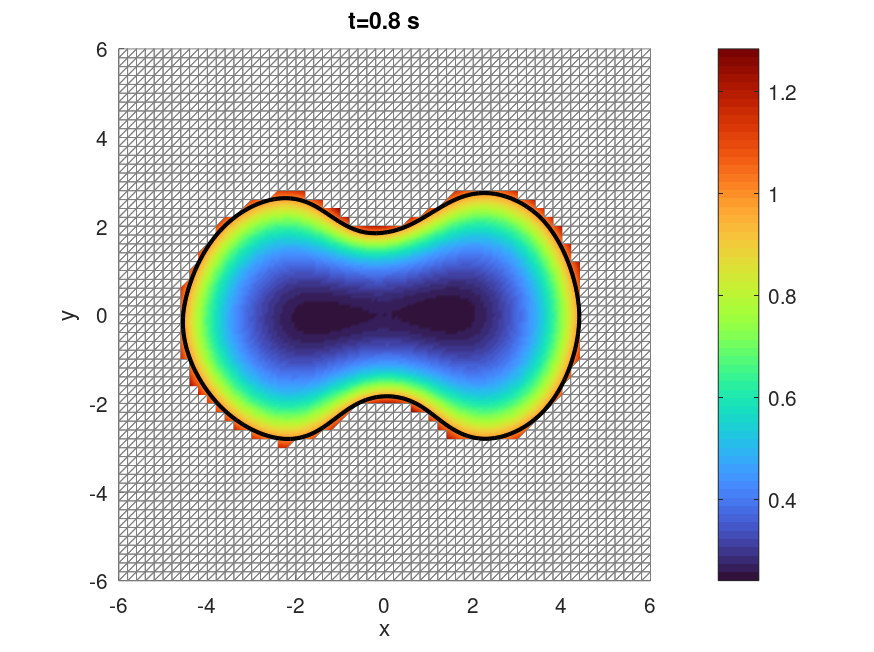
\includegraphics[width=0.4\linewidth]{casoA/nutrientes800}
	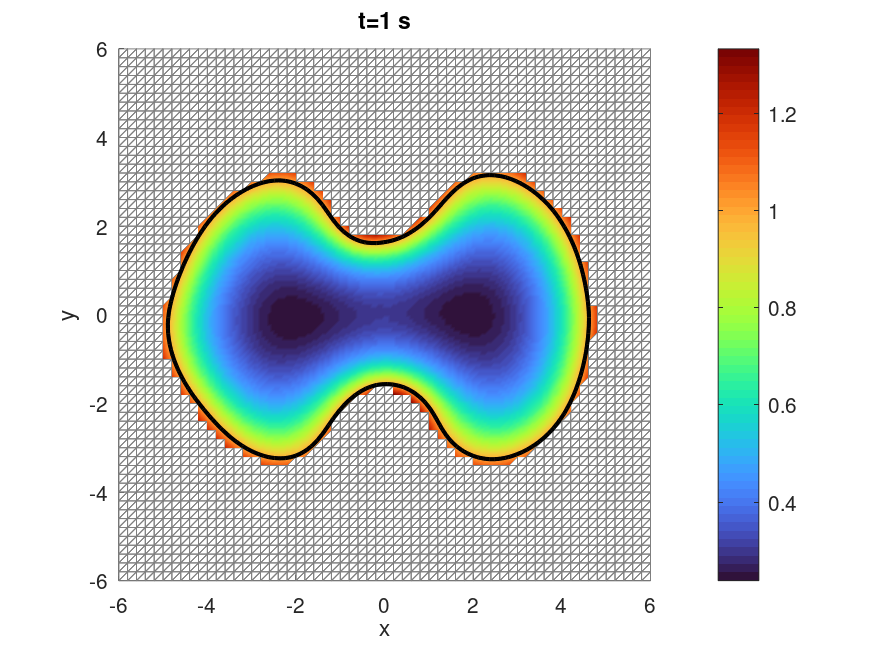
\includegraphics[width=0.4\linewidth]{casoA/nutrientes1000}
	\caption{Evolución de la concentración de nutrientes al interior del tumor de frontera inicial dada por la ecuación \ref{eqn:casoA}, $A=0.5$, $G=20$}
	\label{fig:evolucionnutrientesA}
\end{figure}
\begin{figure}[H]
	\centering
	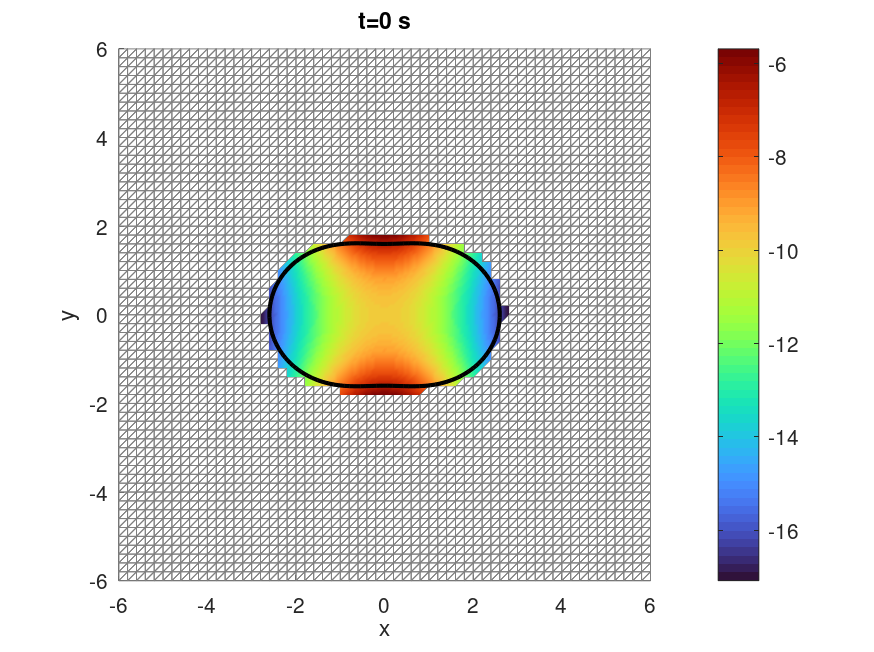
\includegraphics[width=0.4\linewidth]{casoA/presion0}
	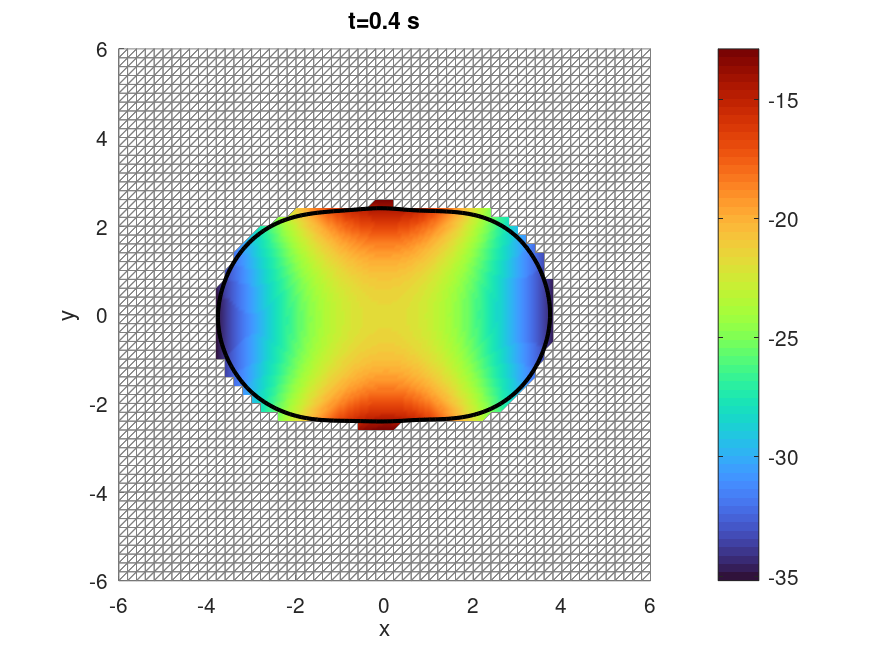
\includegraphics[width=0.4\linewidth]{casoA/presion400}
	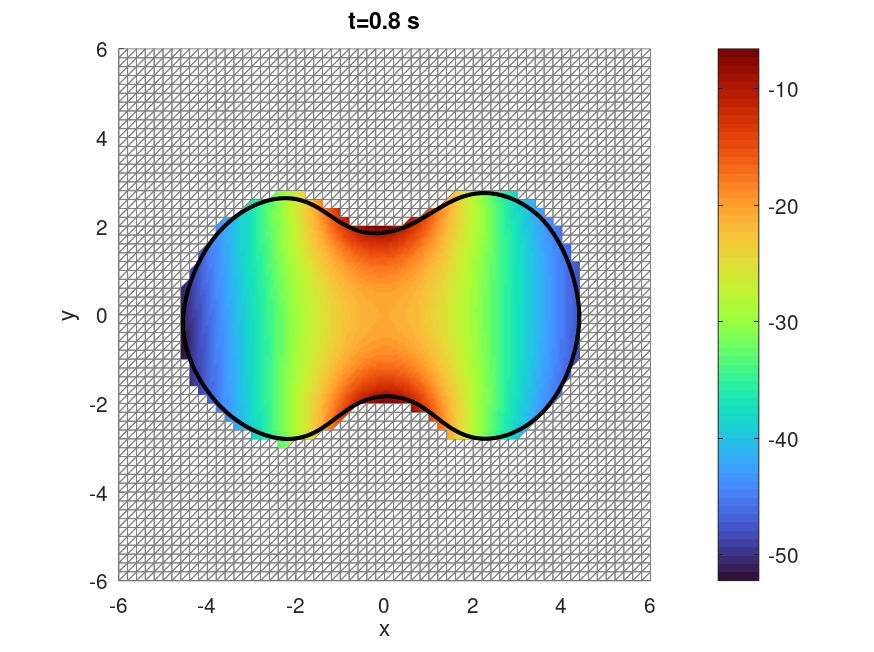
\includegraphics[width=0.4\linewidth]{casoA/presion800}
	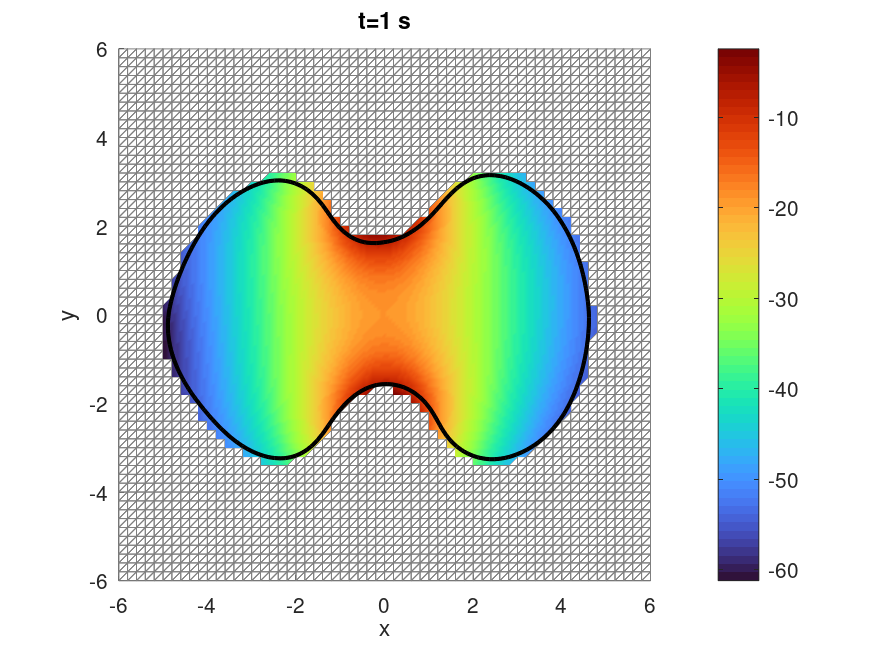
\includegraphics[width=0.4\linewidth]{casoA/presion1000}
	\caption{Evolución de la presión al interior del tumor de frontera inicial dada por la ecuación \ref{eqn:casoA}, $A=0.5$, $G=20$}
	\label{fig:evolucionpresionA}
\end{figure}
En las Figuras \ref{fig:evolucionnutrientesB}-\ref{fig:evolucionpresionB} los valores que identifican el régimen de alta vascularización son $G=-5$, $A=0.8$ y la frontera inicial del tumor está dada por la curva polar 
\begin{equation}
	r= 2 + 0.24\cos(2\theta) + 0.2\sin(2\theta) + 0.12\cos(3\theta) + 0.1\sen(3\theta)+0.08\cos(5\theta)+ 0.14\sen(6\theta)
	\label{eqn:casoB}
\end{equation}
\begin{figure}[H]
	\centering
	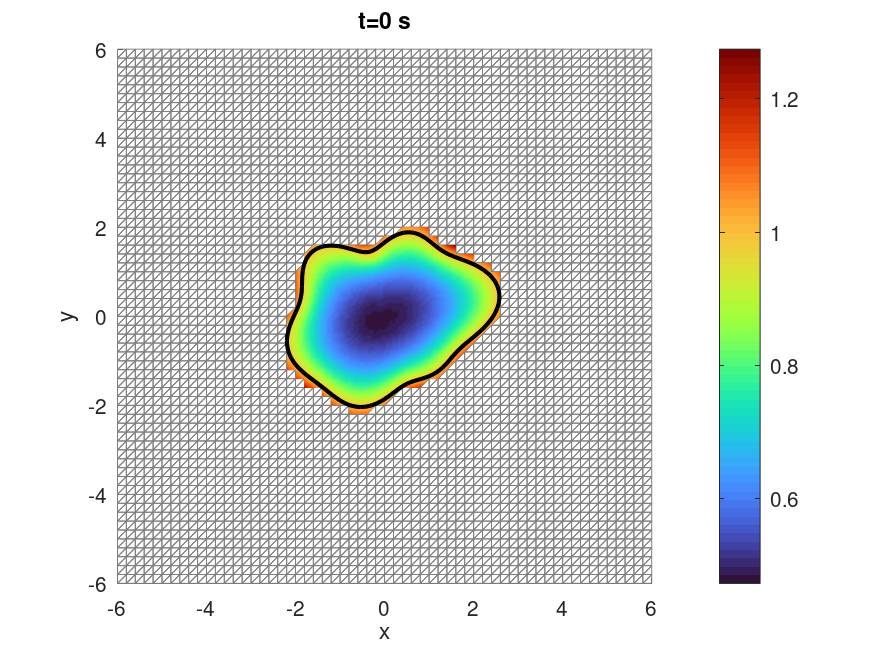
\includegraphics[width=0.4\linewidth]{casoB/nutrientes0}
	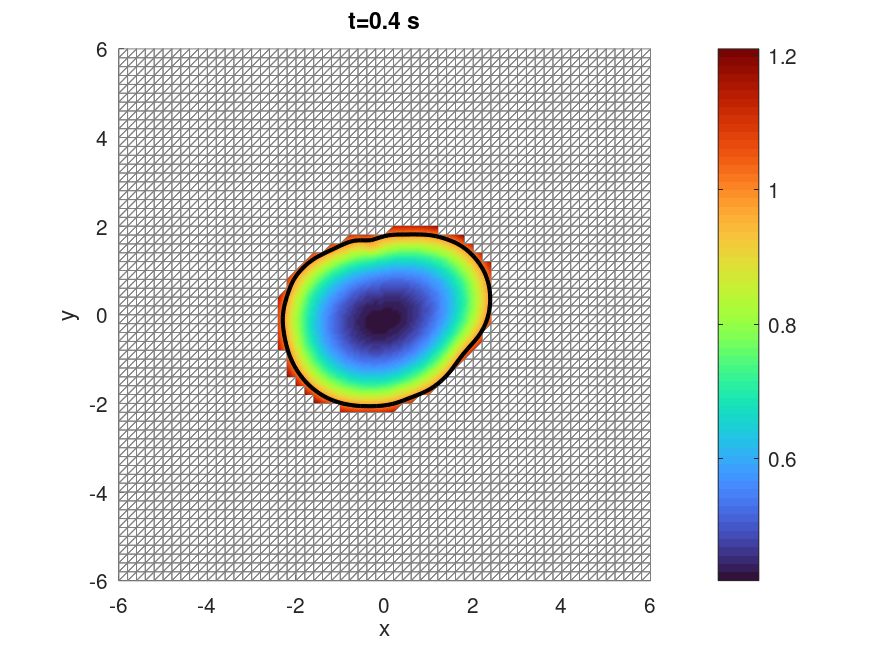
\includegraphics[width=0.4\linewidth]{casoB/nutrientes400}
	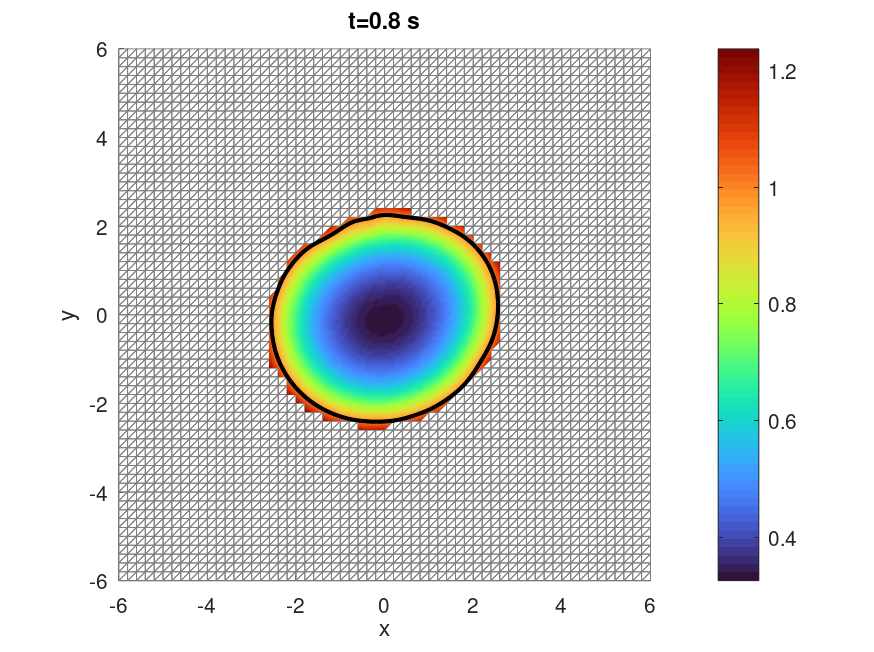
\includegraphics[width=0.4\linewidth]{casoB/nutrientes800}
	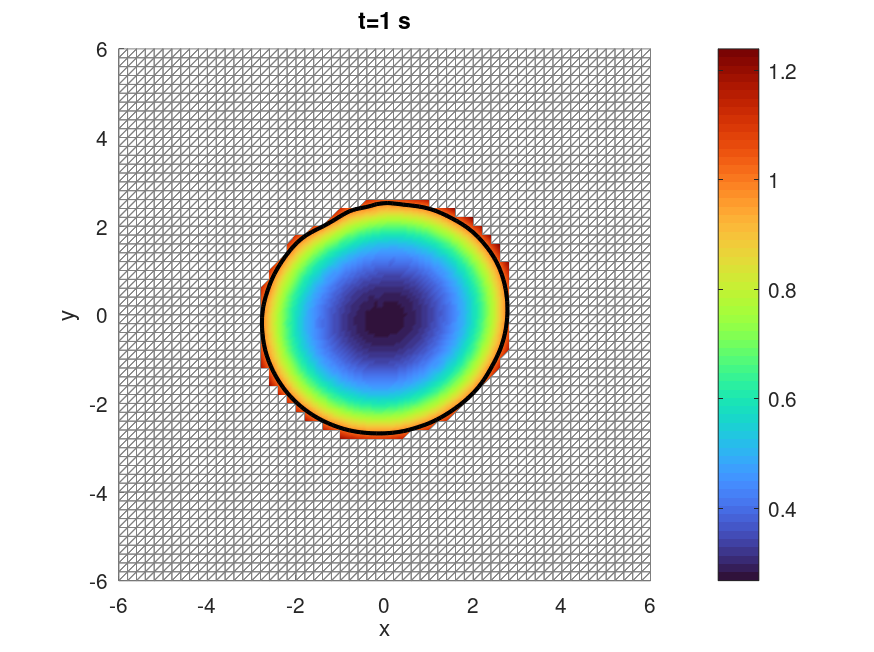
\includegraphics[width=0.4\linewidth]{casoB/nutrientes1000}
	\caption{Evolución de la concentración de nutrientes al interior del tumor de frontera inicial dada por la ecuación \ref{eqn:casoB}, $A=0.8$, $G=-5$}
	\label{fig:evolucionnutrientesB}
\end{figure}
\begin{figure}[H]
	\centering
	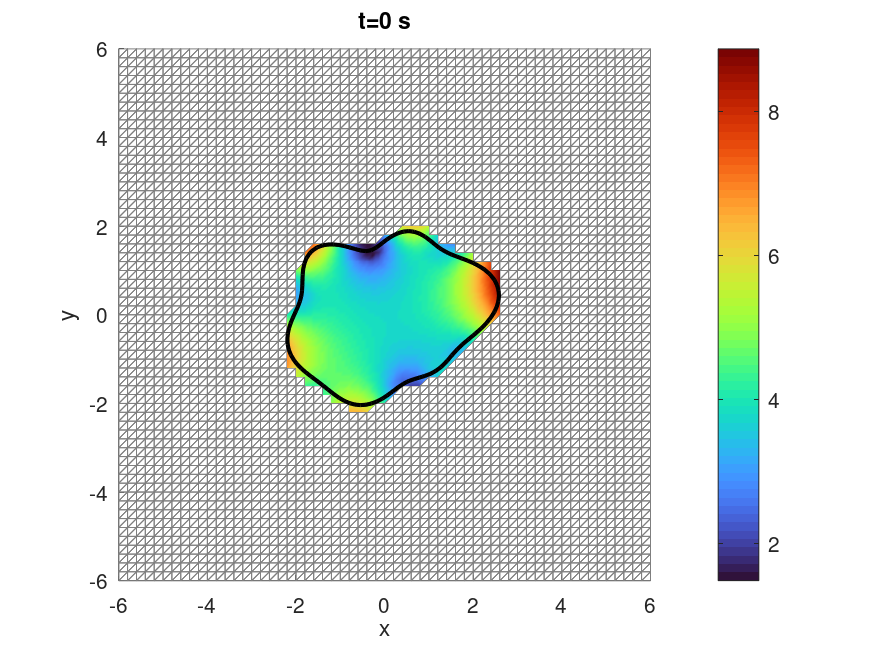
\includegraphics[width=0.4\linewidth]{casoB/presion0}
	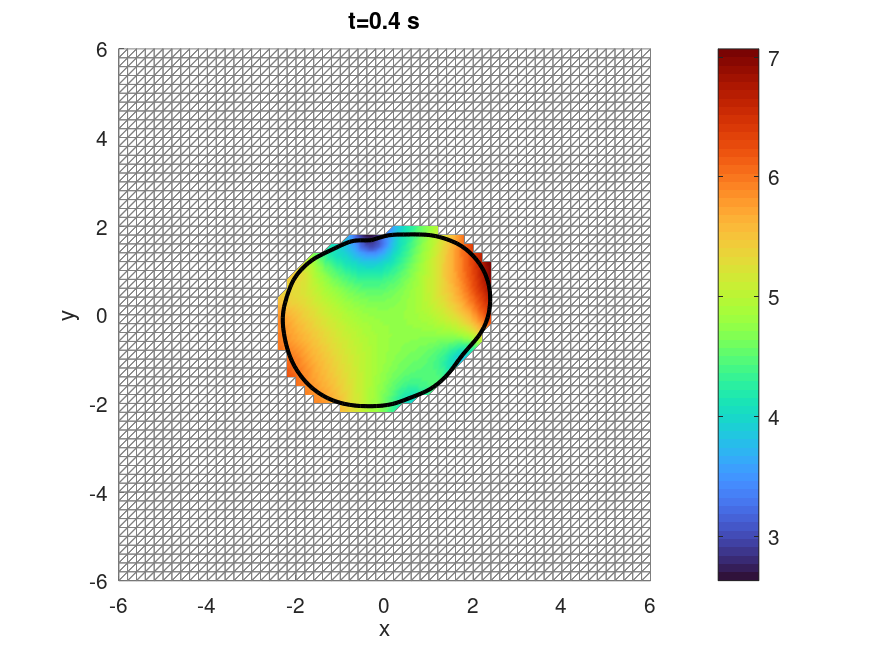
\includegraphics[width=0.4\linewidth]{casoB/presion400}
	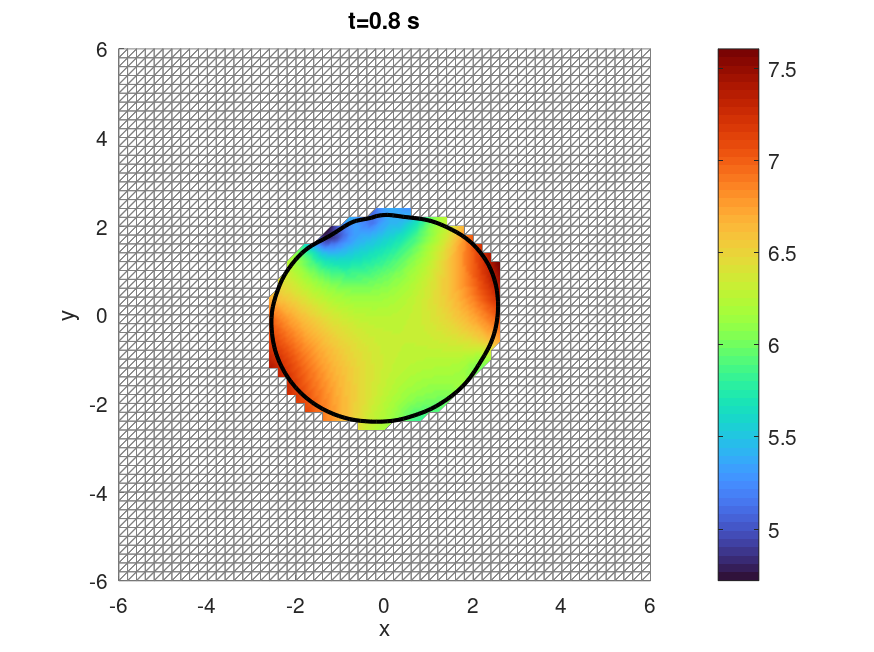
\includegraphics[width=0.4\linewidth]{casoB/presion800}
	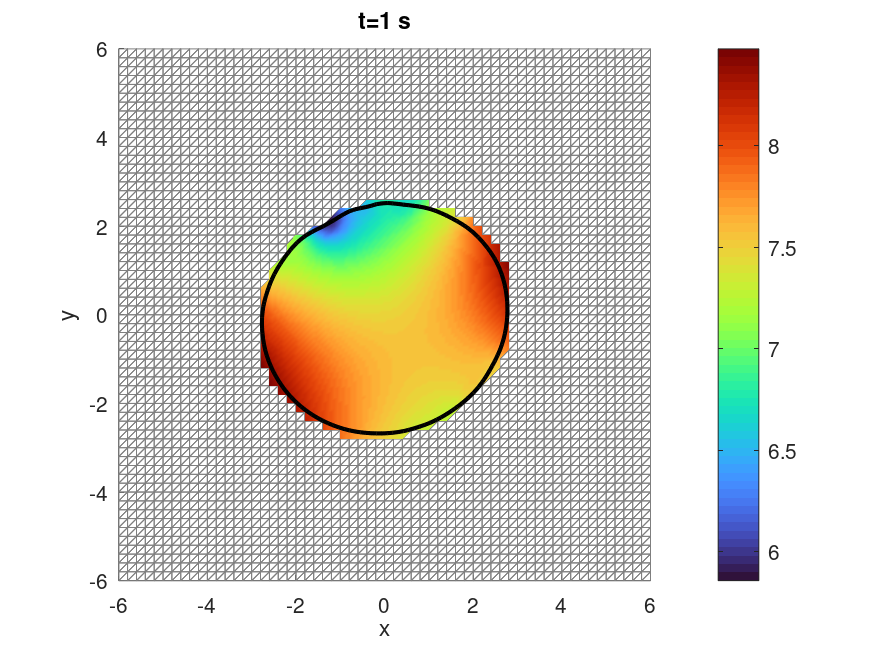
\includegraphics[width=0.4\linewidth]{casoB/presion1000}
	\caption{Evolución de la presión al interior del tumor de frontera inicial dada por la ecuación \ref{eqn:casoB}, $A=0.8$, $G=-5$}
	\label{fig:evolucionpresionB}
\end{figure}
En las Figuras \ref{fig:evolucionnutrientesC}-\ref{fig:evolucionpresionC} se observa el decrecimiento de un tumor con régimen de alta vascularización identificado por $G=-5$, $A=0.2$. y la frontera inicial del tumor está dada por la curva polar 
\begin{equation}
	r = 2 + 0.24\cos(2\theta) + 0.2\sen(2\theta) + 0.12\cos(3\theta)  + 0.1 \sen(3\theta)
	\label{eqn:casoC}
\end{equation}
\begin{figure}[H]
	\centering
	\includegraphics[width=0.4\linewidth]{casoC/nutrientes0}
	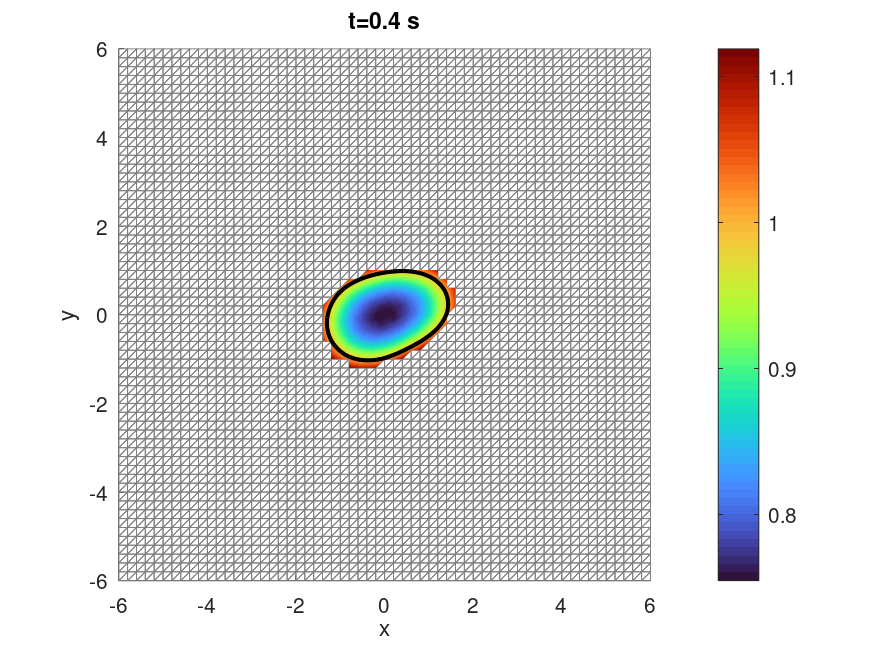
\includegraphics[width=0.4\linewidth]{casoC/nutrientes400}
	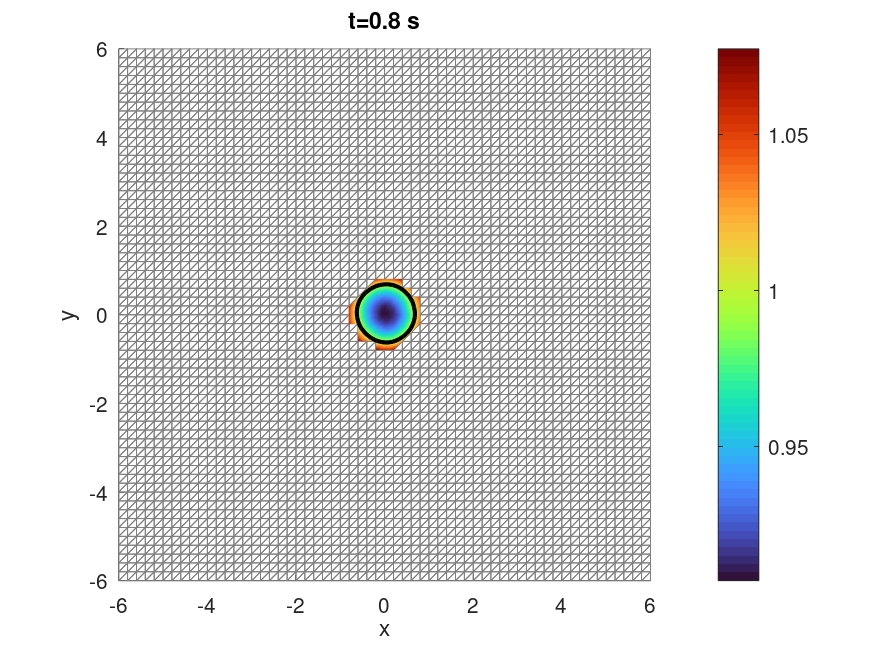
\includegraphics[width=0.4\linewidth]{casoC/nutrientes800}
	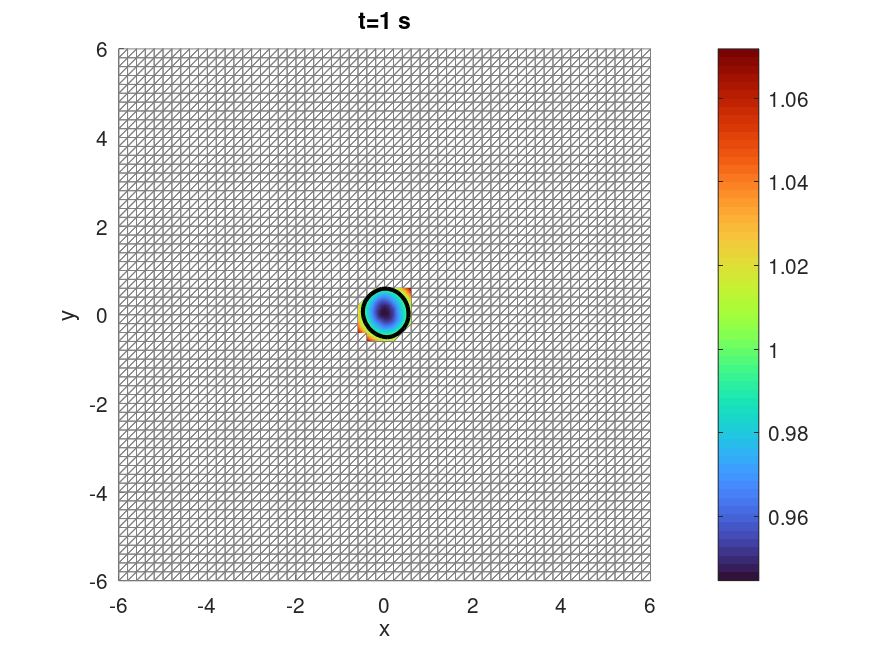
\includegraphics[width=0.4\linewidth]{casoC/nutrientes1000}
	\caption{Evolución de la concentración de nutrientes al interior del tumor de frontera inicial dada por la ecuación \ref{eqn:casoC}, $A=0.2$, $G=-5$} 	
	\label{fig:evolucionnutrientesC}
\end{figure}
\begin{figure}[H]
	\centering
	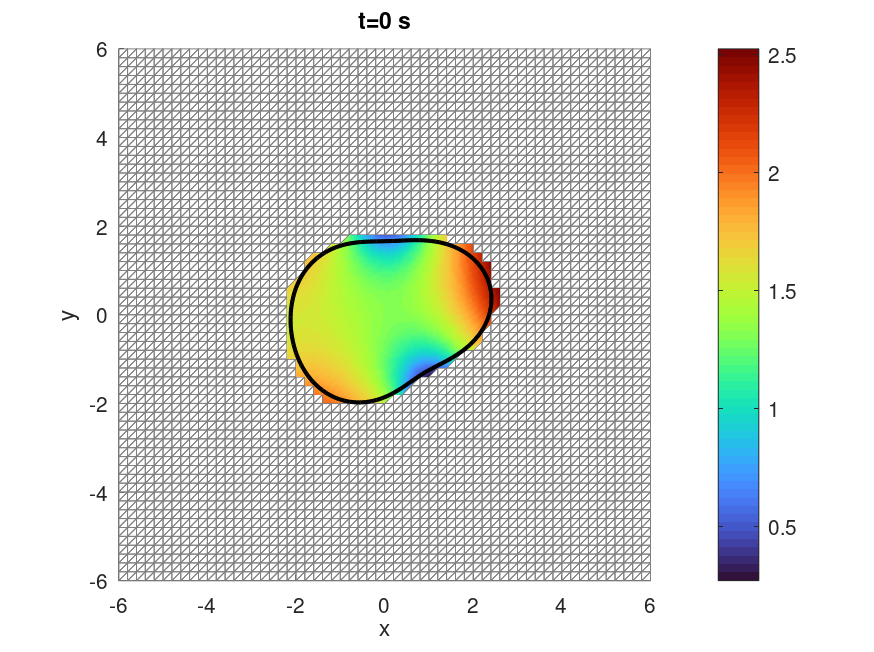
\includegraphics[width=0.4\linewidth]{casoC/presion0}
	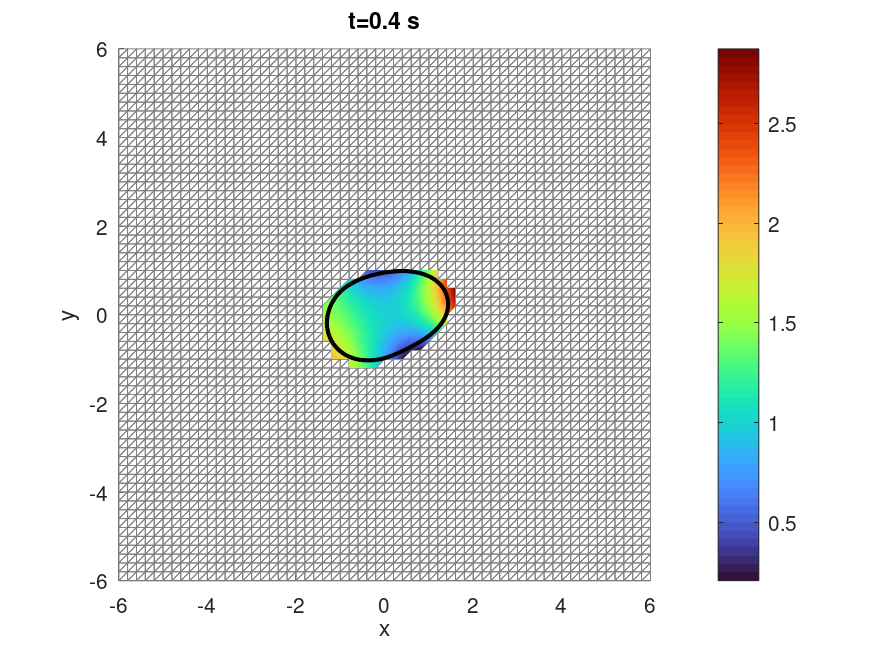
\includegraphics[width=0.4\linewidth]{casoC/presion400}
	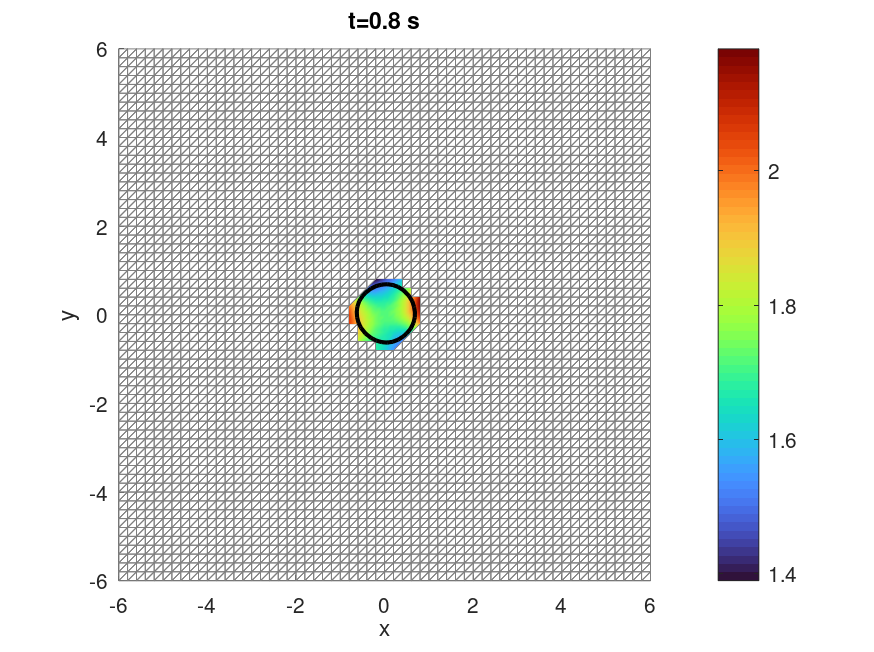
\includegraphics[width=0.4\linewidth]{casoC/presion800}
	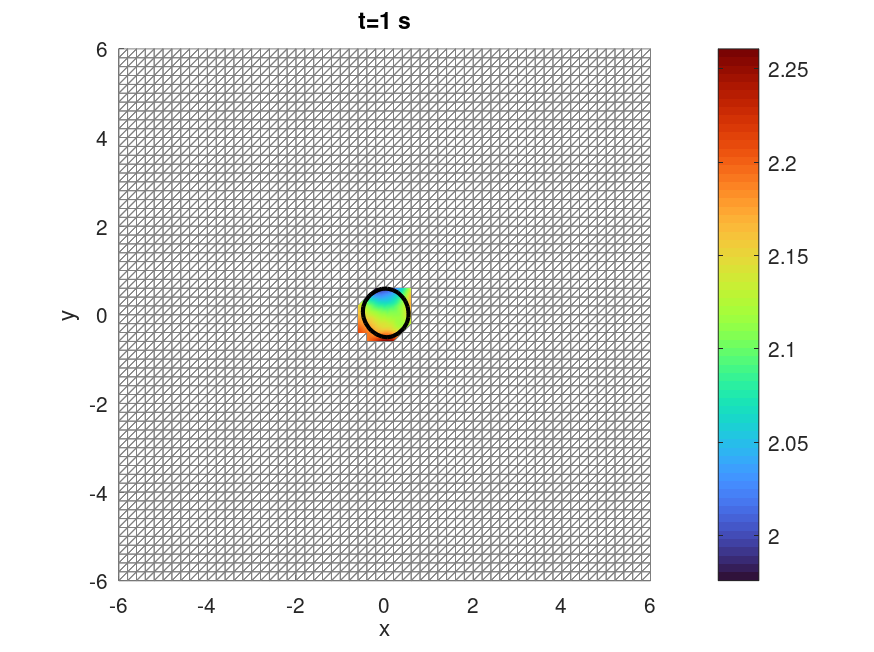
\includegraphics[width=0.4\linewidth]{casoC/presion1000}
	\caption{Evolución de la presión al interior del tumor de frontera inicial dada por la ecuación \ref{eqn:casoC}, $A=0.2$, $G=-5$}	
	\label{fig:evolucionpresionC}
\end{figure}
En las Figuras \ref{fig:evolucionnutrientesD}-\ref{fig:evolucionpresionD} se observa el crecimiento de un tumor con régimen de alta vascularización identificado por $G=-5$, $A=0.8$. y la frontera inicial del tumor está dada por la curva polar mostrada en la ecuación \ref{eqn:casoC}.
\begin{figure}[H]
	\centering
	\includegraphics[width=0.4\linewidth]{casoD/nutrientes0}
	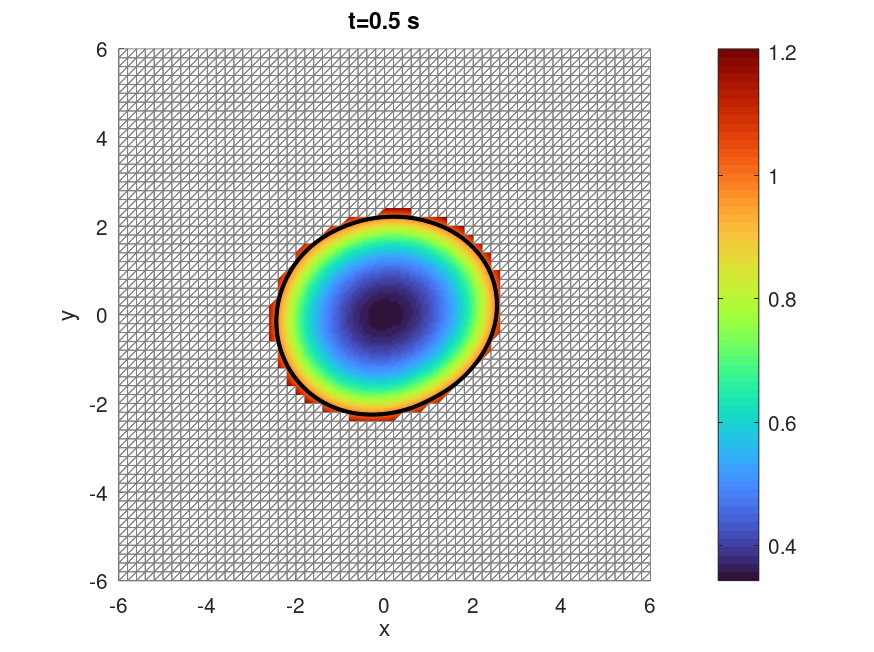
\includegraphics[width=0.4\linewidth]{casoD/nutrientes500}
	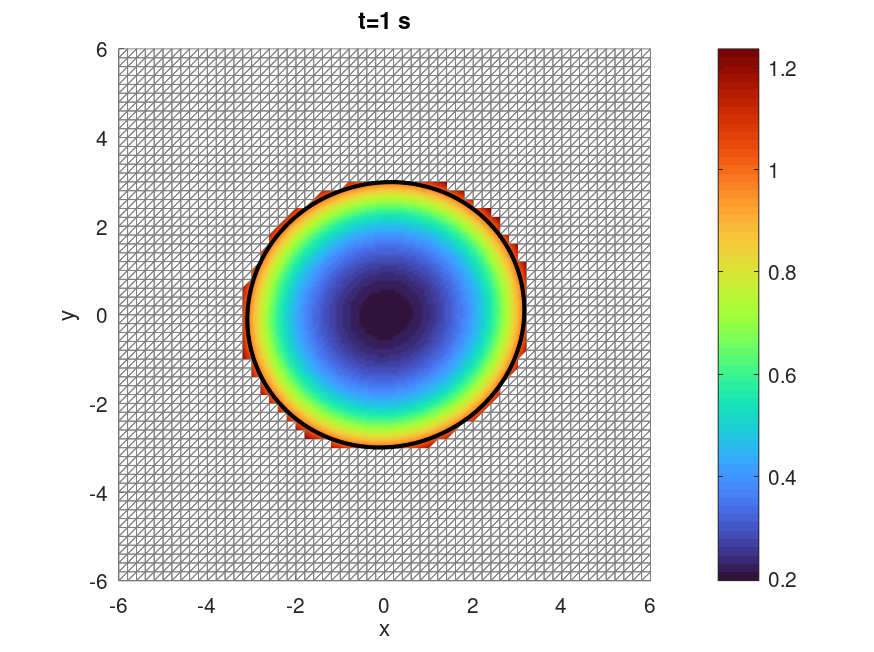
\includegraphics[width=0.4\linewidth]{casoD/nutrientes1000}
	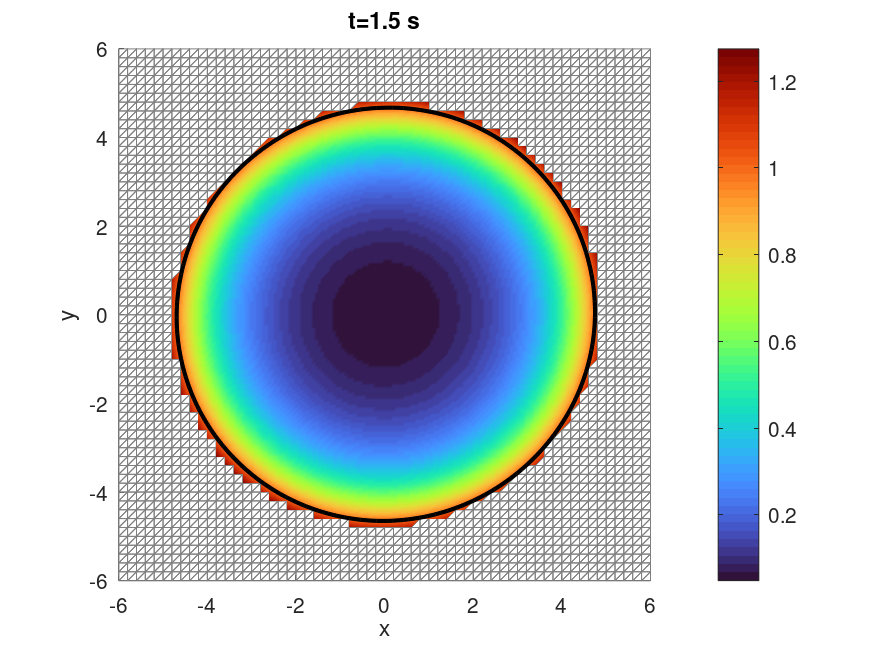
\includegraphics[width=0.4\linewidth]{casoD/nutrientes1500}
	\caption{Evolución de la concentración de nutrientes al interior del tumor de frontera inicial dada por la ecuación \ref{eqn:casoC}, $A=0.8$, $G=-5$} 	
	\label{fig:evolucionnutrientesD}
\end{figure}
\begin{figure}[H]
	\centering
	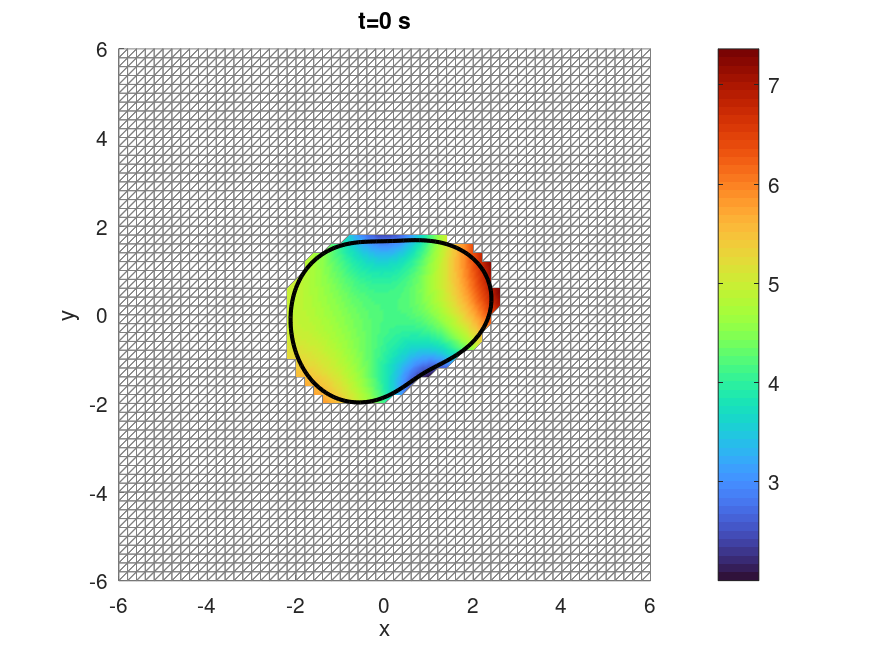
\includegraphics[width=0.4\linewidth]{casoD/presion0}
	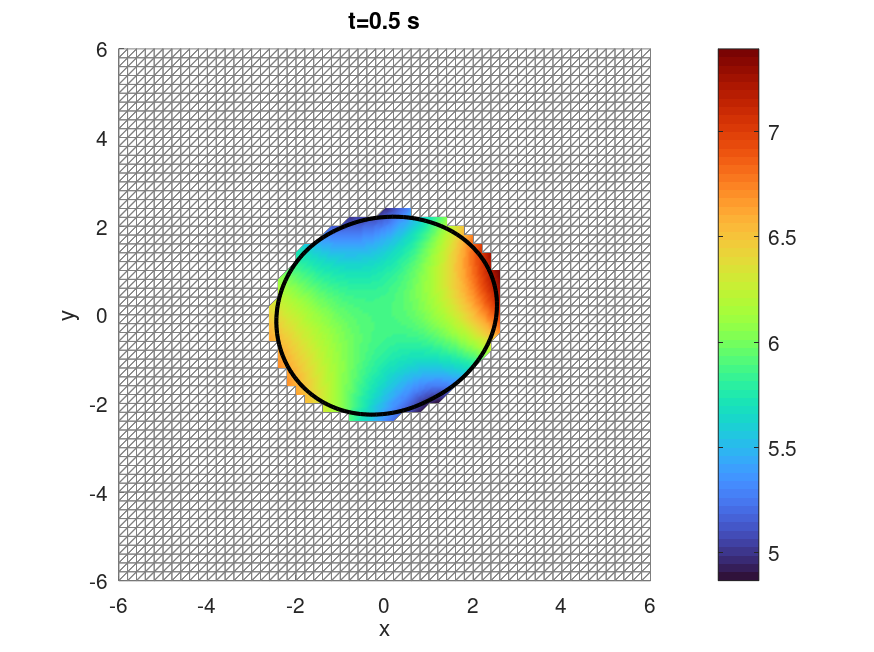
\includegraphics[width=0.4\linewidth]{casoD/presion500}
	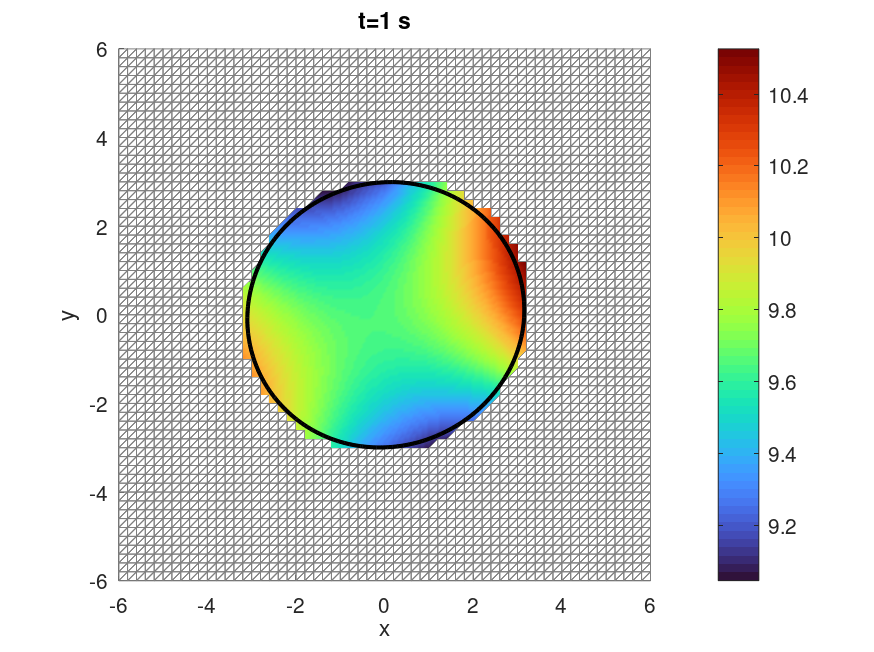
\includegraphics[width=0.4\linewidth]{casoD/presion1000}
	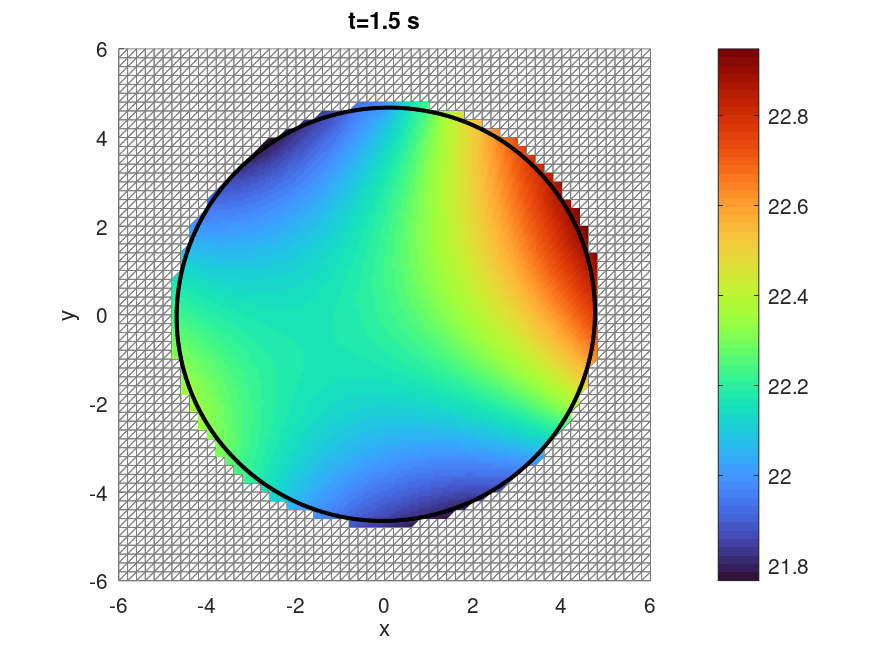
\includegraphics[width=0.4\linewidth]{casoD/presion1500}
	\caption{Evolución de la presión al interior del tumor de frontera inicial dada por la ecuación \ref{eqn:casoC}, $A=0.8$, $G=-5$}	
	\label{fig:evolucionpresionD}
\end{figure}
\comentario{
	\section{Convergencia numérica del problema de Poisson}
	Para las experiencias numéricas se considera resolver el problema $-\Delta u +u = f \text{ en }\Omega, u=g\text{ en }\partial\Omega$ con
	$\Omega = \{x^2+y^2\leq 1/16 \}$ contenido en un dominio fijo  $\mathcal{O}=(-0.5,0.5)^2$. La solución exacta es $u_{ex}=\sen(x)\exp(y)$ si $f=u_{ex}$, y  $g=u_{ex}$.
	
	
	
	\begin{figure}[H]	
		\centering
		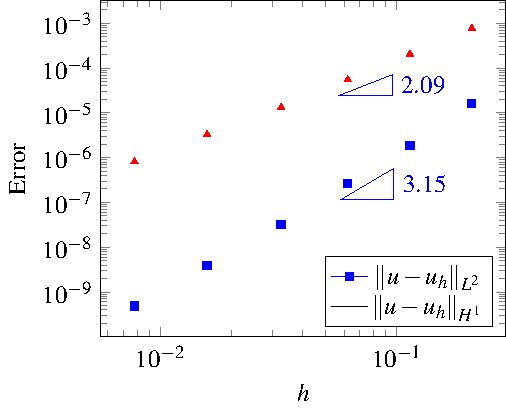
\includegraphics[width=0.4\linewidth]{convergenciafem.pdf}
		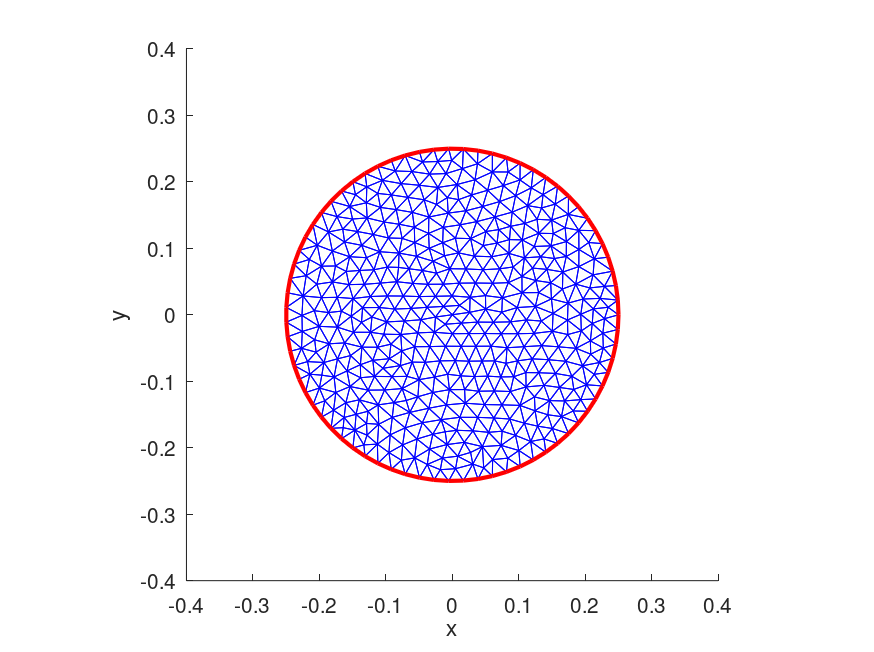
\includegraphics[width=0.4\linewidth]{problemaEDP}
		
	\end{figure}
	
	\begin{figure}[H]
		\centering	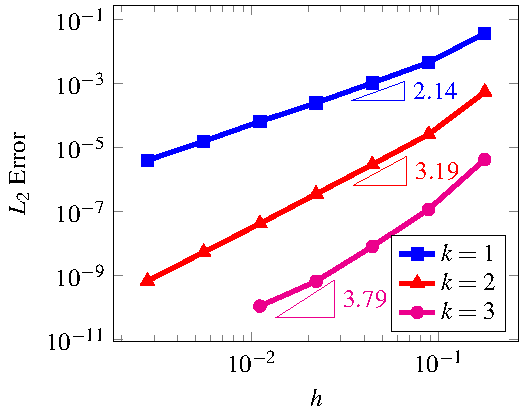
\includegraphics[width=0.4\linewidth]{convergenciaphifemduala}\hfil
		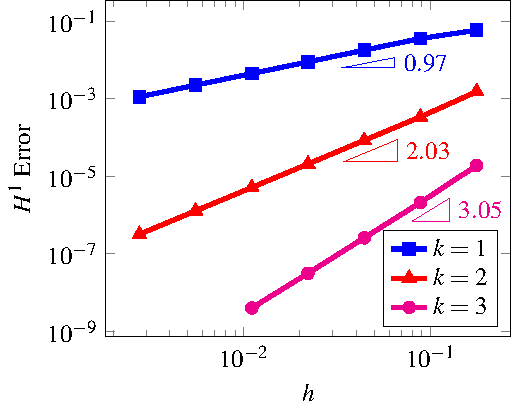
\includegraphics[width=0.4\linewidth]{convergenciaphifemdualb}\\
		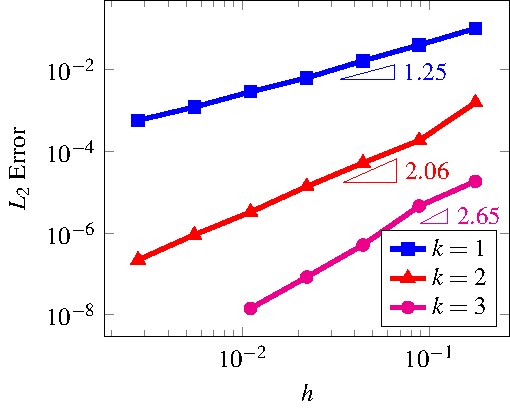
\includegraphics[width=0.4\linewidth]{convergenciaphifemdualc}
		\caption{Convergencia de la solución numérico del problema \ref{eqn:phifemdual}. Izquierda error relativo $L^2$}
		\label{fig:convergenciaphifemduala}
	\end{figure}
	\section{Esquema de estabilización de la curvatura}
	\begin{figure}[H]
		\centering	
		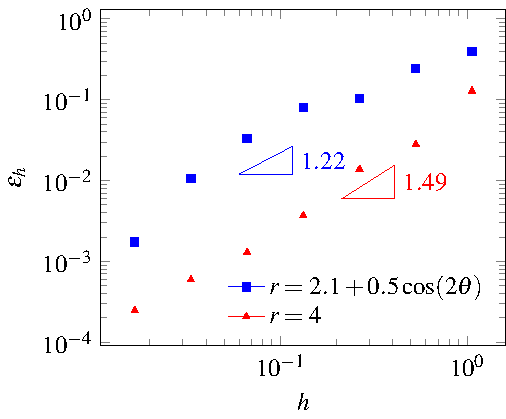
\includegraphics{convergenciacurvaturacirculo}
		\caption{Error en la aproximación de la curvatura de una curva polar $r=f(\theta)$}
		\label{fig:convergenciacurvaturacirculo}
	\end{figure}
	
	\begin{figure}[H]
		\centering
		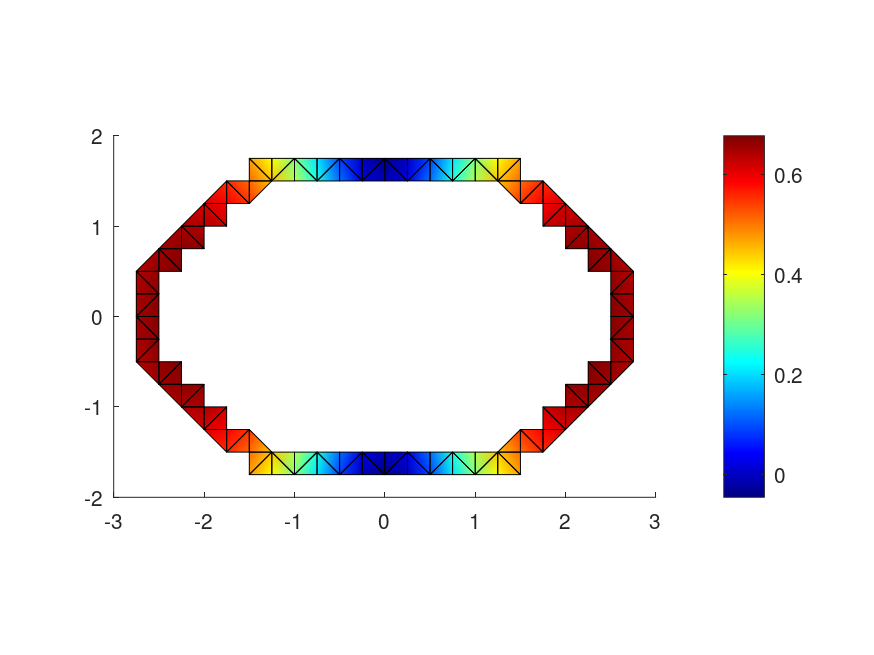
\includegraphics[width=0.7\linewidth]{curvaturaperturbacion}
		\caption{$\Omega_h$ y extensión de la curvatura $K_h$ para $r=2.1 + 0.5\cos(2\theta)$.}
		\label{fig:curvaturaperturbacion}
	\end{figure}
	\begin{figure}[H]
		\centering
		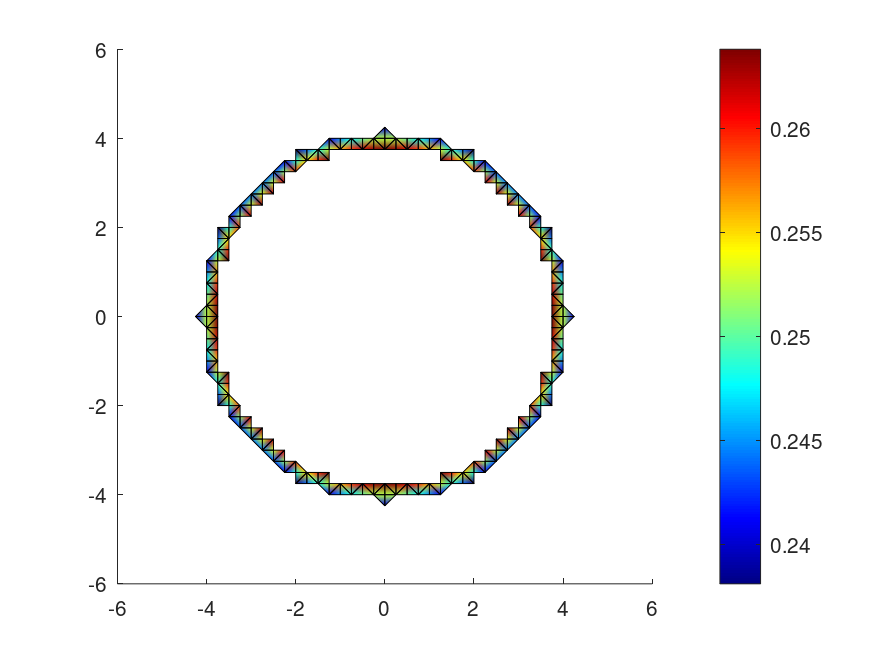
\includegraphics[width=0.7\linewidth]{curvaturacirculo}
		\caption{$\Omega_h$ y extensión de la curvatura $K_h$ para $r=2.1$.		
		}
		\label{fig:curvaturacirculo}
	\end{figure}
	
	
	\subsection{Convergencia, caso frontera libre circular}
	Para las experiencias numéricas se elige una función conjunto de nivel $\phi_0=x^2+y^2-4$ definida en primer caso sobre $D_1=(-4,4)^2$ y luego sobre $D_2=(-4,4)^2\setminus [-0.4,0.4]^2$,  de modo que en el segundo caso no se considera el origen pues la función distancia dirigida $\phi=\sqrt{x^2+y^2}-2$ no es diferenciable en el origen y el orden de convergencia se ve afectado. En la Figura \ref{fig:levelsetcircular} se muestra el orden de convergencia para valores de $h$ correspondiente a una triangulación uniforme con $n=8(2^i)$, subdivisiones para $i=0,1,\ldots, 6$.
	
	\begin{figure}[H]
		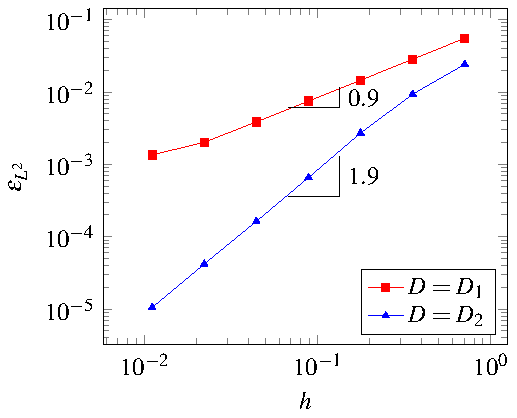
\includegraphics{reinicializacionradioconstantea.pdf}
		~%
		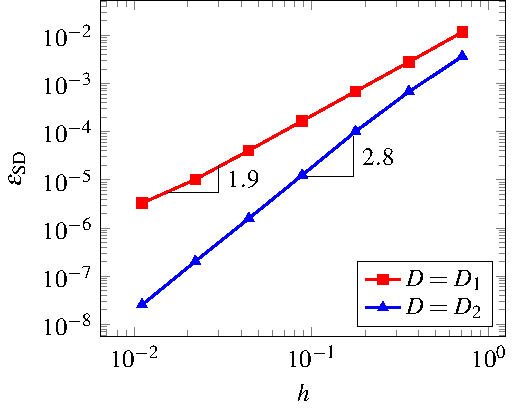
\includegraphics{reinicializacionradioconstanteb.pdf}
		%
		%
		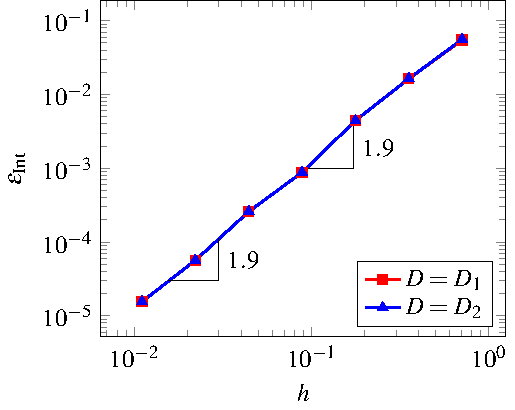
\includegraphics{reinicializacionradioconstantec.pdf}
		~%
		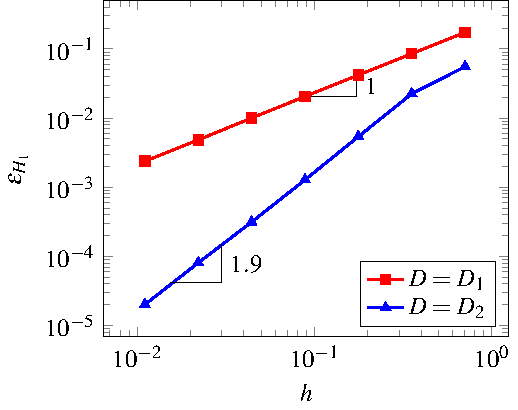
\includegraphics{reinicializacionradioconstanted.pdf}
		\caption{Errores y orden de convergencia de la reinicialización de la función conjunto de nivel}
		\label{fig:levelsetcircular}
	\end{figure}
	
	
	\subsection{Convergencia, caso frontera libre de radio variable}
	Para las experiencias numéricas se elige una función conjunto de nivel \[
	\phi_0=x^2+y^2 - (2.1 + 0.5\cos(2\arctan(\frac{y}{x}))
	\] definida en un dominio banda $D$ tal que $\{\phi_0=0\}\subset D$ de modo que la reinicialización se realice solo en los elementos cercanos a la frontera libre. El dominio banda depende de la triangulación utilizada por lo tanto para comparar errores calculados en malla distintas, utilizaremos el error normalizado por unidad de área, $\dfrac{\epsilon_{SD}}{|D|}$. En la Figura \ref{fig:levelsetvariable} se muestra el orden de convergencia para valores de $h$ correspondiente a una triangulación uniforme con $n=8(2^i)$, subdivisiones para $i=1,\ldots, 6$.
	
	\begin{figure}[H]
		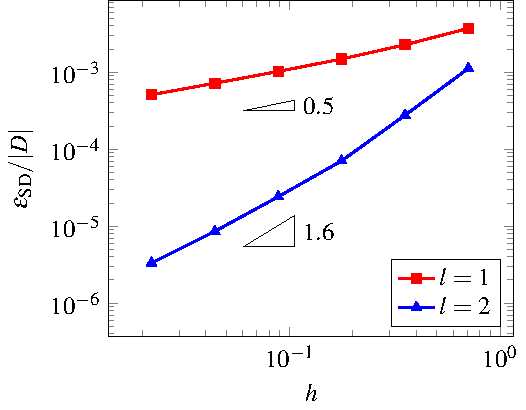
\includegraphics{reinicializacionradiovariablea.pdf}%
		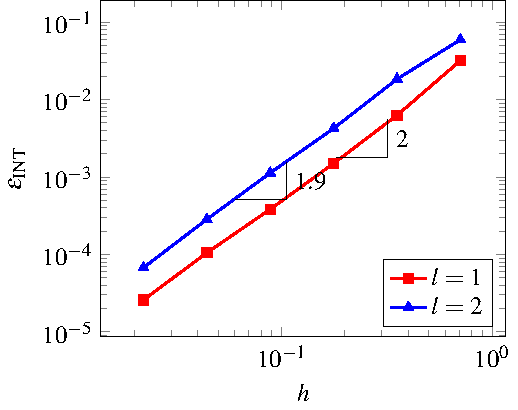
\includegraphics{reinicializacionradiovariableb.pdf}
		\caption{Errores y orden de convergencia de la reinicialización de la función conjunto de nivel}
		\label{fig:levelsetvariable}
	\end{figure}
	
	\subsection{Convergencia, caso frontera con esquinas}
	Siguiendo a \citep{min2010reinitializing} se considera el caso de dos círculos de radio $r$ con centros $C_1=(-a,0)$, $C_2=(a,0)$, ($0<a<r$) tal que se interceptan en $V_1=(0,\sqrt{r^2-a^2})$, $V_2=(0,-\sqrt{r^2-a^2})$, de modo que la frontera libre este formada por la frontera de la unión de dichos círculos. La función distancia dirigida en este caso es
	\[
	\phi(x,y)=\begin{cases}
		-\min \left\{ d((x,y),V_i),i=1,2\right\} &,\text{ si } \frac{x+a}{d((x,y),V_1)}\geq \frac{a}{r} \text{ y }
		\frac{a-x}{d((x,y),V_2)}\geq \frac{a}{r},
		\\
		\min \left\{ d((x,y),C_i),i=1,2\right\}-r&
		,\text{ en otro caso.}
	\end{cases}
	\]
	Como función inicial tenemos 
	\[
	\phi^{0} = \phi \cdot \left[ (x-1)^2+ (y-1)^2 + 0.1\right]
	\]
	%\[
	%\phi^{0,b} = \phi \cdot \left[ 0.5 \sen(6\pi x)\sen (6\pi y) %+ 1\right]
	%\]
	\begin{figure}[H]
		\centering
		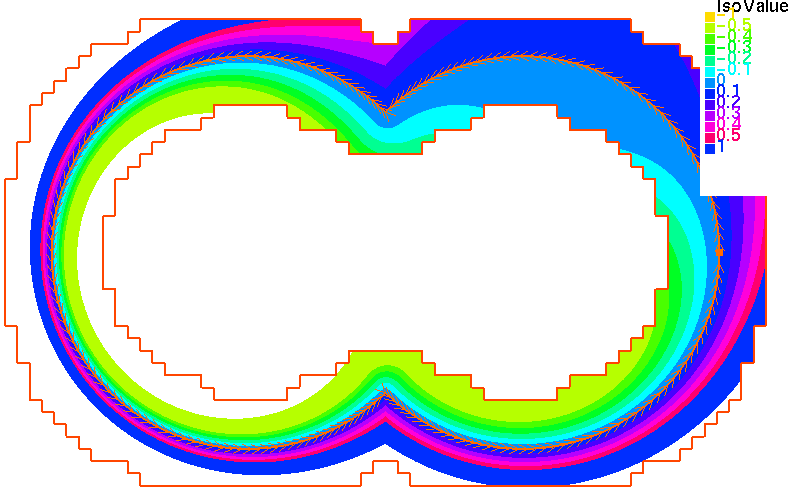
\includegraphics[width=0.7\linewidth]{lsconesquinasphi0amanchas}
		%	\includegraphics[width=0.7\linewidth]{lsconesquinasphi0bmanchas}
		\caption{Curvas de nivel para $\phi^{0}$}
		\label{fig:lsconesquinasphi0amanchas}
	\end{figure}
	
	\begin{figure}[H]
		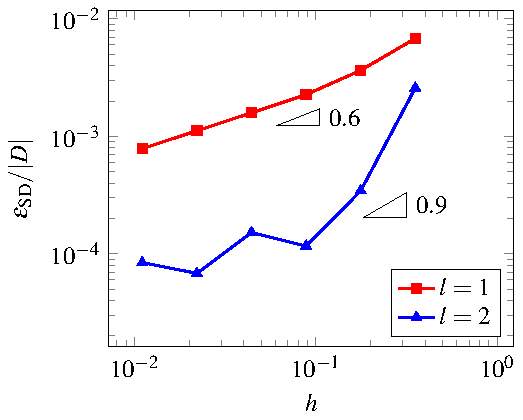
\includegraphics{reinicializacionfronteraesquinaa.pdf}
		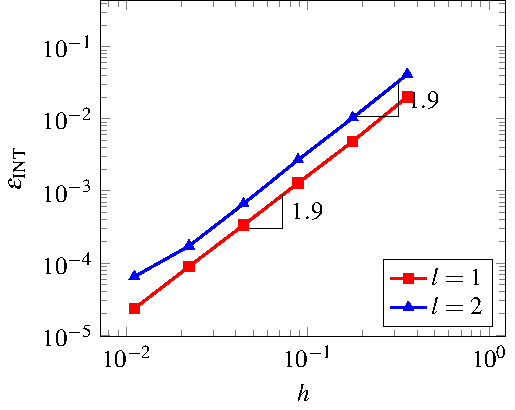
\includegraphics{reinicializacionfronteraesquinab.pdf}
		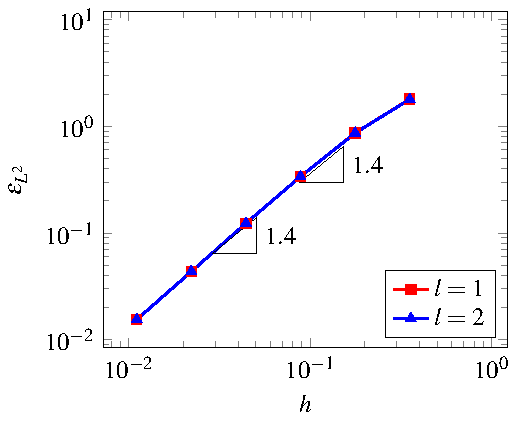
\includegraphics{reinicializacionfronteraesquinac.pdf}
		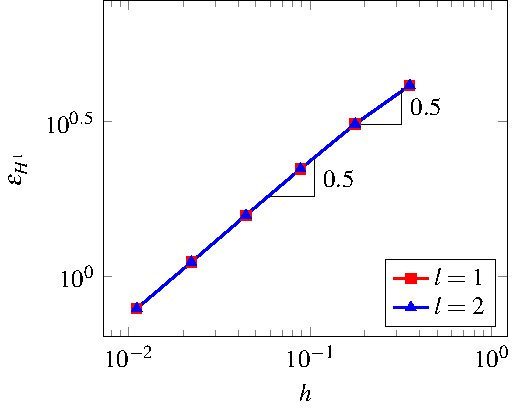
\includegraphics{reinicializacionfronteraesquinad.pdf}
		
		\caption{Errores y orden de convergencia de la reinicialización de la función conjunto de nivel en el caso de una frontera con esquinas o picos.}
		\label{fig:levelsetconesquinas}
	\end{figure}
}

\comentario{
	%%%%%%%%%%%% grafica la frontera libre %%%%%%%%%%%%%%%%%%
	figure;
	[xmesh,~,ymesh,~]=prepare_mesh(p,t);
	x=linspace(-2,2,100);
	y=linspace(-2,2,100);
	[X,Y]=meshgrid(x,y);
	[~,pdeData]=convert_pde_data(p,t,Sh,uh');
	PP=fftri2grid(X,Y,xmesh,ymesh,pdeData{1});
	hold on;
	PE=X;
	%contourf(X,Y,PP,"linewidth",2,"k.-");
	colormap ("turbo"); colorbar ();
	
	%contourf(X,Y,PP,"linewidth",0.5,"b");
	surf(X,Y,PP);
	shading interp;
	%contour(X,Y,PE,[0,0],"linewidth",1,"r-");
	%plot(x, sqrt(x.^2+1)-1,"linewidth",1,"b-",x,1-sqrt(x.^2+1),"linewidth",1,"b-");
	xlabel("x");
	ylabel("y");
	axis("equal");
	view([ 58.065,61.996])
	%title(["t=",num2str(step*i)," s"]);
	print(["extension1.png"])
	
	figure;
	
	[~,pdeData]=convert_pde_data(p,t,Sh,wh');
	PP=fftri2grid(X,Y,xmesh,ymesh,pdeData{1});hold on;
	colormap ("turbo"); colorbar ();
	
	%contourf(X,Y,PP,"linewidth",0.5,"b");
	surf(X,Y,PP);
	shading interp;
	
	%contour(X,Y,PE,[0,0],"linewidth",1,"r-");
	%plot(x, sqrt(x.^2+1)-1,"linewidth",1,"b-",x,1-sqrt(x.^2+1),"linewidth",1,"b-");
	xlabel("x");
	ylabel("y");
	axis("equal");
	%title(["t=",num2str(step*i)," s"]);
	view([ 58.065,61.996])
	print(["extension2.png"])
}
%\chapter{\MakeUppercase{Conclusiones y Recomendaciones}}
%%\chapter{Conclusiones}
%\thispagestyle{fancy}
%%\addcontentsline{toc}{chapter}{Conclusiones}
%\begin{itemize}
%	\item Se ha demostrado la existencia y unicidad de la solución numérica del problema de la concentración de nutrientes al interior de un tumor con frontera determinada por una función conjunto de nivel.
%	\item Se ha demostrado la existencia y unicidad de la solución numérica del problema de la presión intracelular en un tumor con frontera determinada por una función conjunto de nivel.
%	\item Se ha encontrado una extensión desde una curva de nivel a un dominio rectangular de la velocidad de crecimiento tumoral mediante una aproximación por elementos finitos. 
%	\item Se ha implementado un algoritmo para la evolución del crecimiento tumoral por medio del método de elementos finitos definidos sobre un domino rectangular.
%	\item Se ha realizado la simulación numérica del crecimiento tumoral para diferentes fronteras y niveles de vascularización, y los resultados obtenidos concuerdan con los comportamientos registrados en la literatura: crecimiento acelerado del tumor, estabilización alrededor de una solución estacionario o la extinción del tumor. 
%\end{itemize}

\chapter{\MakeUppercase{Conclusiones}}
%\chapter{\MakeUppercase{Conclusiones y Recomendaciones}}
%\chapter{Conclusiones y Recomendaciones}
\thispagestyle{fancy}
%%\addcontentsline{toc}{chapter}{Conclusiones}
\section{Conclusiones}
\begin{itemize}
	\item Se ha demostrado la existencia y unicidad de la solución numérica del problema de la concentración de nutrientes al interior de un tumor con frontera determinada por una función conjunto de nivel.
	\item Se ha demostrado la existencia y unicidad de la solución numérica del problema de la presión intracelular en un tumor con frontera determinada por una función conjunto de nivel.
	\item Se ha encontrado una extensión desde una curva de nivel a un dominio rectangular de la velocidad de crecimiento tumoral mediante una aproximación por elementos finitos. 
	\item Se ha implementado un algoritmo para la evolución del crecimiento tumoral por medio del método de elementos finitos definidos sobre un domino rectangular.
	\item Se ha realizado la simulación numérica del crecimiento tumoral para diferentes fronteras y niveles de vascularización, y los resultados obtenidos concuerdan con los comportamientos registrados en la literatura: crecimiento acelerado del tumor, estabilización alrededor de una solución estacionario o la extinción del tumor. 
\end{itemize}
\section{Recomendaciones}
\begin{itemize}
	\item Es preciso desarrollar el análisis teórico del error que valide las experiencias numéricas presentadas en este trabajo.
	\item Es posible resolver la ecuación de evolución  en una región muy próxima a la frontera libre pues solo interesa el comportamiento de una curva de nivel y no es necesario resolver sobre todo el dominio rectangular, este enfoque se conoce en la literatura como \emph{narrow band level set method}.
	\item Es importante que la función conjunto de nivel  $\phi$ conserve la propiedad de distancia dirigida en una región próxima a la frontera libre $\Gamma$ mediante algún proceso de reinicialización que controle el valor de $\|\nabla \phi \|$.
	\item Es necesario considerar el proceso de necrosis, es decir si la concentración de nutrientes cae por debajo de un umbral dado entonces las células de tumor mueren, esto da lugar a problemas de Poisson con término fuente. 
\end{itemize}

%%\chapter{\MakeUppercase{Recomendaciones}}\thispagestyle{fancy}
\chapter{Recomendaciones}\thispagestyle{fancy}
%\addcontentsline{toc}{chapter}{Recomendaciones}
\begin{itemize}
	\item Es preciso desarrollar el análisis teórico del error que valide las experiencias numéricas presentadas en este trabajo.
	\item Es posible resolver la ecuación de evolución  en una región muy próxima a la frontera libre pues solo interesa el comportamiento de una curva de nivel y no es necesario resolver sobre todo el dominio rectangular, este enfoque se conoce en la literatura como \emph{narrow band level set method}.
	\item Es importante que la función conjunto de nivel  $\phi$ conserve la propiedad de distancia dirigida en una región próxima a la frontera libre $\Gamma$ mediante algún proceso de reinicialización que controle el valor de $\|\nabla \phi \|$.
	\item Es necesario considerar el proceso de necrosis, es decir si la concentración de nutrientes cae por debajo de un umbral dado entonces las células de tumor mueren, esto da lugar a problemas de Poisson con término fuente. 
\end{itemize}

%\bibliographystyle{IEEEtranN}
%\bibliography{levelset}
\renewcommand{\bibsection}{\chapter*{\MakeUppercase{\bibname}}}
%\chapter*{\MakeUppercase{Referencias bibliográficas}}
%\chapter*{Referencias bibliográficas}
%\chapter*{Bibliografía}
%\renewcommand{\bibsection}{\chapter{\bibname}}
\thispagestyle{fancy}
\addcontentsline{toc}{chapter}{\MakeUppercase{\bibname}}
%\addcontentsline{toc}{chapter}{\bibname}
\bibliographystyle{IEEEtranN}
\bibliography{levelset}

%\printbibliography[title={Referencias},heading=bibintoc]
%\printbibliography[title={Referencias},heading=bibintoc]
%\printbibliography[title={Referencias},keyword=spanish,heading=bibintoc]word=spanish,heading=bibintoc]

%\printbibliography[title={Referencias},heading=bibintoc]

%\printbibliography
%\appendix

%%\chapter{Programas implementados}
\chapter*{\MakeUppercase{Anexos}}
%\chapter*{Anexos}
\addcontentsline{toc}{chapter}{\MakeUppercase{Anexos}}
%\addcontentsline{toc}{chapter}{Anexos}
\thispagestyle{fancy}

\noindent Anexo 1: Evolución del crecimiento tumoral con frontera circular \dotfill 1

\noindent Anexo 2: Evolución del crecimiento tumoral con frontera dada por un conjunto de nivel  \dotfill 2

\noindent Anexo 3: Script para generar graficas de presión y concentración de nutrientes  \dotfill 13
\chapter*{Anexo 1: Evolución del crecimiento tumoral con frontera circular}
\setcounter{page}{1}
\thispagestyle{fancy}
%\addcontentsline{toc}{section}{Anexo 1: Evolución del crecimiento tumoral con frontera circular}
El siguiente script se ejecutó en Octave 8.2 \footnote{\url{https://www.octave.org}}.
\begin{lstlisting}
R0=4;
A=.0;  G=20.0;
xx = linspace(0,50,100);
fvdp = @(y,t) G*besseli(1,y)./besseli(0,y)-0.5*A*G*y;
t = linspace (0, 1, 101);
R = lsode (fvdp, R0, t);
V=fvdp(R,t);
figure;
[hAy,hLine1,hLine2] = plotyy(t,V,t,R);
ylabel(hAy(1),'Velocidad') % eje izquierdo
ylabel(hAy(2),'Radio del tumor') % eje derecho
xlabel('t')
title('Evolución del tumor')
\end{lstlisting}
\chapter*{Anexo 2: Evolución del crecimiento tumoral con frontera dada por un conjunto de nivel}
\thispagestyle{fancy}
%\addcontentsline{toc}{section}{Anexo 2: Evolución del crecimiento tumoral con frontera dada por un conjunto de nivel}
El siguiente programa se ejecutó con FreeFem 4.12 \footnote{\url{https://freefem.org}}, genera archivos con información de la presión y la concentración de nutrientes que pueden ser cargados a Octave para el posproceso.

\begin{lstlisting}[language=C++]
load "UMFPACK64"
include "ffmatlib.idp"
///////////////////////////////////////////
// resuelve con elementos P2
///////////////////////////////////////////
verbosity = 1;
int MALLADIAGONAL=0;
int MALLACRUZ=1;
int tipomalla = MALLADIAGONAL;
int i=0;
int bandwidth=8;
int maxit = 101;
real step = 0.005;
int gradPol;
macro gradPol1()
gradPol=1;
func funckappa=P1;
func funcPhih=P1;
func funcVh=P1;
func funcSh=P1;
//EOM
macro gradPol2()
gradPol=2;
func funckappa=P2;
func funcPhih=P2;
func funcVh=P2;
func funcQ1h=P2;
func funcQ2h=P1;
func funcSh=P1;
func funcZh=P2;
//EOM
macro gradPol3()
gradPol=1;
func funckappa=P1;
func funcPhih=P4;
func funcVh=P3;
func funcSh=P3;
//EOM
gradPol2;
////////////////////////////////////////////////////////
/////// parametros de la ecuaciones de campo   ////////
////////////////////////////////////////////////////////
real beta;
real A, G;  
////////////////////////////////////////////////////////
real iso= 0.0 ;
real[int] viso=[iso];
real eps1 = 1.e-6;
///////////////////////////////////////////////////////
//////////////////// frontera inicial /////////////////
///////////////////////////////////////////////////////
macro experimentoA()
A=0.5;  G=20.0;  
maxit = 1001;
step = 0.001;
string caso="casoA";
func real rt(real t){       
	return (2.1 + 0.5*cos(2*t));
}
//EOM
macro experimentoB()
A=0.8;  G=-5.0; 
maxit = 1001;
step = 0.001; 
string caso="casoB";
func real rt(real t){
	return (2 + 0.24*cos(2*t) + 0.2*sin(2*t) + 0.12*cos(3*t)
	+ 0.1*sin(3*t)+0.08*cos(5*t)+ 0.14*sin(6*t));
	
}
//EOM
macro experimentoC()
A=0.2;  G=-5.0; 
maxit = 1001;
step = 0.001;  
string caso="casoC";
func real rt(real t){
	return (2 + 0.24*cos(2*t) + 0.2*sin(2*t) + 0.12*cos(3*t)
	+ 0.1*sin(3*t));              
}
//EOM

experimentoC

border circ(t=0,2*pi){ x=rt(t)*cos(t); y=rt(t)*sin(t);}

func theta=atan2(y,x);

func phi = sqrt(square(x)+square(y)) - (rt(theta));

int m;
{
	int n=60;
	
	mesh ThGlob,Th, ThGam;
	
	func real Meshsize(mesh & Th)
	{
		fespace Ph(Th,P0);
		Ph h=hTriangle;
		return h[].max;
	}
	
	fespace Vphi(ThGlob,funcPhih);
	fespace Vind1Glob(ThGlob,P1); 
	fespace Vind0Glob(ThGlob,P0);

	fespace Bh(ThGam,funckappa); // funcion de curvatura
	fespace BhGlob(ThGlob,funckappa);
	fespace Vh(Th,funcVh); 
	fespace VhP1(Th,P1);
	fespace VphiP1(ThGlob,P1);
	fespace VhGam(ThGam,funcVh); 
	fespace VphiGam(ThGam,funcPhih); 
	fespace Xh(Th,funcPhih); 
	fespace Qh(ThGam,funcVh); 
	fespace ShGam(ThGam,funcSh); 
	fespace Sh(ThGlob,funcSh); 
	
	Vphi phih;
	Vphi nx,ny;
	Bh kappa ;
	int[int] n2o1,n2o2,Tnb2ThGlob;
	int[int] R;
	int bandwidth = 5;
	
	macro Laplacian(u) (dxx(u) + dyy(u)) // EOM
	
	macro calculaNutrientes(phih,variable){
		Vh u,v;
		real sigma=20.0;
		fespace Vind0(Th,P0);
		Vind0 ind0 = ind0Glob; 
		solve phifem(u,v,solver=sparsesolver)
		= int2d(Th)( (dx(phih)*u + phih*dx(u))*(dx(phih)*v + phih*dx(v)) +
		(dy(phih)*u + phih*dy(u))*(dy(phih)*v + phih*dy(v)) +
		phih^2*u*v
		)
		- int1d(Th)( ( (dx(phih)*u + phih*dx(u))*N.x + (dy(phih)*u + phih*dy(u))*N.y)*(phih*v) )
		+ intalledges(Th)(sigma*hTriangle*(InternalEdge)*(mean(ind0)>0)
		* jump( (dx(phih)*u + phih*dx(u))*N.x + (dy(phih)*u + phih*dy(u))*N.y )
		* jump( (dx(phih)*v + phih*dx(v))*N.x + (dy(phih)*v + phih*dy(v))*N.y )/nTonEdge)    
		+ int2d(Th)( phih*v )     
		+ int2d(Th,2) ( sigma*hTriangle^2*( 
		dxx(phih)*u+2*dx(phih)*dx(u)+phih*dxx(u) + dyy(phih)*u+2*dy(phih)*dy(u)+phih*dyy(u) 
		-phih*u    
		)*(         
		dxx(phih)*v+2*dx(phih)*dx(v)+phih*dxx(v) + dyy(phih)*v+2*dy(phih)*dy(v)+phih*dyy(v) 
		-phih*v           
		))
		- int2d(Th,2) ( sigma*hTriangle^2*( 
		dxx(phih)*v+2*dx(phih)*dx(v)+phih*dxx(v) + dyy(phih)*v+2*dy(phih)*dy(v)+phih*dyy(v) 
		-phih*v
		))      
		;
		variable = 1 +u*phih;
	}// EOM
	
	macro calculaVariable(phih,variable,f,g,beta){
		fespace Vind0(Th,P0);
		Vind0 ind0 = ind0Glob; 
		real gamma=20, sigma=20.0;
		varf varA(u,v)= int2d(Th)( (dx(u)*dx(v)+dy(u)*dy(v)) + beta*u*v ) 
		+ int2d(Th,2) ( gamma/square(hTriangle)* u*v ) 
		+ int2d(Th,2) ( sigma*square(hTriangle)*(Laplacian(u)-beta *u )*(Laplacian(v)-beta *v) )
		- int1d(Th) ((dx(u)*N.x + dy(u)*N.y)*v )
		+ intalledges(Th)(sigma*hTriangle*(InternalEdge)*(mean(ind0)>0)*
		jump(dx(u)*N.x+dy(u)*N.y)*jump(dx(v)*N.x+dy(v)*N.y)/nTonEdge)
		+ int2d(Th)( f*v )
		+ int2d(Th,2)(-sigma*square(hTriangle)*f*(Laplacian(v)-beta *v) 
		+ (gamma/square(hTriangle)*g*v) )
		;
		varf varB(p,v)= -int2d(ThGam)(gamma/(hTriangle^3)*phih*p*v); 
		varf varD(p,q)=  int2d(ThGam)(gamma/(hTriangle^4)*phih*phih*p*q)
		- int2d(ThGam)(gamma/(hTriangle^3)*phih*g*q) ;
		
		matrix mA, mB, mD, M;
		real[int] U(Vh.ndof+Qh.ndof), F(Vh.ndof+Qh.ndof);
		
		mA=varA(Vh,Vh);
		mB=varB(Qh,VhGam);      
		mB=I1*mB;    
		mD=varD(Qh,Qh);
		M=[[mA,mB],[mB',mD]];  
		set(M, solver=sparsesolver);        
		F(0:Vh.ndof-1)=varA(0,Vh);
		F(Vh.ndof:Vh.ndof+Qh.ndof-1)=varD(0,Qh);
		U =M^-1*F;
		variable[]=U(0:Vh.ndof-1);  
	}// EOM
		
	macro extenderVariable(Tnb,phih,Vh,VhGam,Qh,variable,f,gD,gN){
		matrix IVh=interpolate(VhGam,Vh,t=true,inside=1);
		fespace Vind0(Tnb,P0);
		Vind0 ind0 = ind0Glob; 
		real gamma=20,sigma=20;
		varf varA(u,v)= int2d(Tnb)(  
		( (dx(phih)^2*dx(u) + dx(phih)*dy(phih)*dy(u))*dx(v) 
		+ (dx(phih)*dy(phih)*dx(u) + dy(phih)^2*dy(u) )*dy(v)  )  ) 
		+ int2d(Tnb,2) ( gamma/square(hTriangle)* u*v ) 
		+ intalledges(Tnb)(sigma*hTriangle*(InternalEdge)*(mean(ind0)>0)*
		jump(dx(u)*N.x+dy(u)*N.y)*jump(dx(v)*N.x+dy(v)*N.y)/nTonEdge)
		+ int1d(Tnb) ((gN)*v )	 
		+ int2d(Tnb)( f*v )
		+ int2d(Tnb,2)( (gamma/square(hTriangle)*gD*v) )  ;
		varf varB(p,v)= -int2d(ThGam)(gamma/(hTriangle^3)*phih*p*v); 
		varf varD(p,q)=  int2d(ThGam)(gamma/(hTriangle^4)*phih*phih*p*q)
		- int2d(ThGam)(gamma/(hTriangle^3)*phih*gD*q) ;
		
		matrix mA, mB, mD, M;
		real[int] U(Vh.ndof+Qh.ndof), F(Vh.ndof+Qh.ndof);
		
		mA=varA(Vh,Vh);
		mB=varB(Qh,VhGam);      
		mB=IVh*mB;    
		mD=varD(Qh,Qh);
		M=[[mA,mB],[mB',mD]];
		set(M, solver=sparsesolver);  
		F(0:Vh.ndof-1)=varA(0,Vh);
		F(Vh.ndof:Vh.ndof+Qh.ndof-1)=varD(0,Qh);
		U =M^-1*F;
		variable[]=U(0:Vh.ndof-1);     
	}// EOM
		
	macro curvaturaP2(phih,Bh,BhGlob,ThGam,kappa,Gam2Glob){
		
		int[int] Curv2Glob;
		int[int] R1 = restrict(Bh, BhGlob, Gam2Glob);
		
		VindGam ind2=1;
		Vind1Glob ind0=0;
		ind0[](RGam1)=ind2[];
		mesh ThCurv = trunc(ThGlob,(ind0>0),split=1,new2old = Curv2Glob);
		mesh ThCurvP1 = trunc(ThCurv,1,split=2);
		
		fespace BhGam1(ThCurvP1,P1);
		fespace BhGam2(ThCurv,P2);
		int[int] R2 = restrict(BhGam2, BhGlob, Curv2Glob);
		BhGam2 kappaP2 = 0;
		mesh Tw;
		BhGam1 kappaP1,N0nb = 0;
		matrix IP1P2 = interpolate(BhGam2, BhGam1,t=true);
		matrix IP2P1 = interpolate(BhGam1, BhGam2,t=true);
		for (int i = 0; i < kappaP1.n; i++){
			N0nb[][i] = 1; 
			Tw = trunc(ThCurvP1, abs(N0nb)>0, split=1, label=2);            
			kappaP1[][i]= -int2d(Tw)( ( dx(phih)*dx(N0nb) + dy(phih)*dy(N0nb) )
			/( sqrt(eps1^2 + (dx(phih))^2 + (dy(phih))^2 ) ) )
			/  int2d(Tw)( N0nb );    
			N0nb[][i] = 0; 
		}
		
		kappaP2[] = IP2P1*kappaP1[]; 
		BhGlob kappaGlob;
		kappaGlob[](R2) = kappaP2[];
		kappa = 0;
		kappa[] = kappaGlob[](R1);
	} // EOM
	macro curvaturaP1(phih,Bh,BhGlob,ThGam,kappa,Gam2Glob){
		
		int[int] Curv2Glob;
		int[int] R1 = restrict(Bh, BhGlob, Gam2Glob);
		
		VindGam ind2=1;
		
		Vind1Glob ind0=0;
		ind0[](RGam1)=ind2[];
		
		mesh ThCurvP1 = trunc(ThGlob,(ind0>0),split=1,new2old = Curv2Glob);
		
		fespace BhGam1(ThCurvP1,P1);
		int[int] R2 = restrict(BhGam1, BhGlob, Curv2Glob);
		mesh Tw;
		BhGam1 kappaP1,N0nb = 0; 
		for (int i = 0; i < kappaP1.n; i++){
			N0nb[][i] = 1; 
			Tw = trunc(ThCurvP1, N0nb>0, split=1, label=2);        
			kappaP1[][i]= -int2d(Tw)( ( dx(phih)*dx(N0nb) + dy(phih)*dy(N0nb) )
			/( sqrt(eps1^2 + (dx(phih))^2 + (dy(phih))^2 ) ) )
			/  int2d(Tw)( N0nb );
			
			N0nb[][i] = 0;     
		}
		BhGlob kappaGlob;
		
		kappaGlob[](R2) = kappaP1[];
		kappa = 0;
		kappa[] = kappaGlob[](R1);
		
	} // EOM
		
	Vind1Glob ind1Glob;
	Vind0Glob ind0Glob;
	int[int] Gam2Glob;
	int[int] Th2Glob;
	fespace VindGam(ThGam,P1);
	int[int] RGam1,RGlob ;
	
	////////////////////////// inicio de las iteraciones /////////////////////////////
	ThGlob=square(n,n,[12*x-6,12*y-6],flags=tipomalla);// 2 diagonales de izq a der
	real meshsiz=Meshsize(ThGlob); //maximal size of a mesh triangle
	cout<<"maximal size of a mesh triangle h="<<meshsiz<<endl;
	
	phih = phi;
	
	int it;
	real instante ;

	savemesh(ThGlob,caso+"/ThGlob.msh");
	ffSaveVh(ThGlob,Vphi,caso+"/Vphi.txt");
	
	for (it=0; it<maxit; it++) {  
		instante=it*step;
		cout<<"Iteracion "<<it+1<<"  t = "<<instante<<endl;
		////////////////////////////////////////////////////// 
		//     Definicion de regiones y fronteras
		//////////////////////////////////////////////////////  
		
		ind1Glob=(phih<1e-10); //1 inside Omega1, 0 outside
		ind0Glob=(ind1Glob<0.9)&&(ind1Glob>0.1); 
		
		ThGam = trunc(ThGlob,ind0Glob==1,split=1,new2old = Gam2Glob);
		ThGam = change(ThGam,flabel = (( phih(x,y) < 0 ) ? 1 : 2 )); // borde interior : 1, borde exterior : 2
		ThGlob = change(ThGlob,fregion = 1+ind0Glob );
		
		RGam1 = restrict(VindGam, Vind1Glob,Gam2Glob);
		
		Th = trunc(ThGlob,ind1Glob>0,split=1,new2old = Th2Glob);  
		Th = change(Th,fregion= 1+ (ind0Glob==1) );
		
		RGlob = restrict(VhP1, VphiP1, Th2Glob);
		
		matrix I1=interpolate(VhGam,Vh,t=true,inside=1);
		Vh presion, nutrientes;
		VhGam nD = 1;
		Vh fn = 0;
		beta = 1.;  
		ShGam vN, vP, vD;
		
		Vphi nabla;
		
		if (gradPol==1){
			curvaturaP1(phih,Bh,BhGlob,ThGam,kappa,Gam2Glob);
		}
		else{
			curvaturaP2(phih,Bh,BhGlob,ThGam,kappa,Gam2Glob);
		}
		  
		calculaNutrientes(phih,nutrientes);  
		
		nD = kappa-A*G*0.25*(x*x+y*y);
		beta = 0; 
		fn=0;
		
		calculaVariable(phih,presion,fn,nD,beta);
		
		viso=[0.25];
		
		Sh S1, S2;
		
		ShGam N1 = dx(phih)/sqrt(eps1^2 + dx(phih)^2+dy(phih)^2);
		ShGam N2 = dy(phih)/sqrt(eps1^2 + dx(phih)^2+dy(phih)^2);
		ShGam Vx = -dx(presion)+G*dx(nutrientes)-0.5*A*G*x;
		ShGam Vy = -dy(presion)+G*dy(nutrientes)-0.5*A*G*y;
		vD = N1*Vx + N2*Vy;
		extenderVariable(ThGlob,phih,Sh,ShGam,ShGam,S1,0,N1*vD,0);
		extenderVariable(ThGlob,phih,Sh,ShGam,ShGam,S2,0,N2*vD,0);
	
		VphiGam phihGam  = phih;
		ffSaveData(phih,caso+"/phih"+it+".txt"); 
		savemesh(Th,caso+"/Th"+it+".msh");
		ffSaveVh(Th,Vh,caso+"/Vh"+it+".txt");
		ffSaveData(nutrientes,caso+"/Vhnutrientes"+it+".txt"); 
		ffSaveData(presion,caso+"/Vhpresion"+it+".txt"); 
		
		Vphi phihtmp;   
		phihtmp= convect([S1,S2],-step,phih);  
		phih = phihtmp;    
	}

}
\end{lstlisting}
\chapter*{Anexo 3: Script para generar graficas de presión y concentración de nutrientes}
\thispagestyle{fancy}
%\addcontentsline{toc}{section}{Anexo 3: Script para generar graficas de presión y concentración de nutrientes}
Para generar la graficas en Octave es necesario copiar los archivos de la librería\\ ffmatlib \footnote{\url{https://github.com/samplemaker/freefem_matlab_octave_plot/tree/public/release-v2.0/demos/ffmatlib}}.

\begin{lstlisting}
graphics_toolkit qt
addpath('./ffmatlib');
maxit = 1001;
step = 0.001;
[p0,b0,t0,nv0,nbe0,nt0,labels0]=ffreadmesh('ThGlob.msh');
Vphi=ffreaddata('Vphi.txt');
for i=0:100:maxit-1
clf;
phih=ffreaddata(['phih',num2str(i),'.txt']);
[p,b,t,nv,nbe,nt,labels]=ffreadmesh(['Th',num2str(i),'.msh']);
Vh=ffreaddata(['Vh',num2str(i),'.txt']);
Vhpresion=ffreaddata(['Vhpresion',num2str(i),'.txt']);
Vhnutrientes=ffreaddata(['Vhnutrientes',num2str(i),'.txt']);
%%%%%%%%%%%%% grafica el mallado%%%%%%%%%%%%%%%%%%%%%%%%
ffpdeplot(p0,b0,t0,'Mesh','on','Boundary','off', ...
'XLim',[-6 6],'YLim',[-6 6],'MColor',[0.5,0.5,0.5]);
hold on;
%%%%%%%%%%%% grafica la concentracion de nutrientes %%%%
ffpdeplot(p,b,t,'VhSeq',Vh,'Mesh','on','XYData',Vhnutrientes,...
'Mesh','off','Boundary','off', ...
'XLim',[-6 6],'YLim',[-6 6],'ColorBar','on','ColorMap','turbo');
%%%%%%%%%%%% grafica la frontera libre %%%%%%%%%%%%%%%%%%
[xmesh,~,ymesh,~]=prepare_mesh(p0,t0);
x=linspace(-6,6,100);
y=linspace(-6,6,100);
[X,Y]=meshgrid(x,y);
[~,pdeData]=convert_pde_data(p0,t0,Vphi,phih');
PP=fftri2grid(X,Y,xmesh,ymesh,pdeData{1});
contour(X,Y,PP,[0,0],"linewidth",2,"k-");
xlabel("x");
ylabel("y");
axis("equal");
title(["t=",num2str(step*i)," s"]);
print(["nutrientes",num2str(i),".png"])
clf;
%%%%%%%%%%%%% grafica el mallado%%%%%%%%%%%%%%%%%%%%%%%%
ffpdeplot(p0,b0,t0,'Mesh','on','Boundary','off', ...
'XLim',[-6 6],'YLim',[-6 6],'MColor',[0.5,0.5,0.5]);
hold on;
%%%%%%%%%%%% grafica la presion intracelular %%%%%%%%%%%%
ffpdeplot(p,b,t,'VhSeq',Vh,'Mesh','on','XYData',Vhpresion,...
'Mesh','off','Boundary','off', ...
'XLim',[-6 6],'YLim',[-6 6],'ColorBar','on','ColorMap','turbo');
%%%%%%%%%%%% grafica la frontera libre %%%%%%%%%%%%%%%%%%
contour(X,Y,PP,[0,0],"linewidth",2,"k-");
xlabel("x");
ylabel("y");
axis("equal");
title(["t=",num2str(step*i)," s"]);
print(["presion",num2str(i),".png"])
endfor
\end{lstlisting}


\end{document}
